	%%% The main file. It contains definitions of basic parameters and includes all other parts.

%% Settings for single-side (simplex) printing
% Margins: left 40mm, right 25mm, top and bottom 25mm
% (but beware, LaTeX adds 1in implicitly)
\documentclass[12pt,a4paper,fleqn]{report}
\setlength\textwidth{145mm}
\setlength\textheight{247mm}
\setlength\oddsidemargin{15mm}
\setlength\evensidemargin{15mm}
\setlength\topmargin{0mm}
\setlength\headsep{0mm}
\setlength\headheight{0mm}
% \openright makes the following text appear on a right-hand page
\let\openright=\clearpage

%% Settings for two-sided (duplex) printing
% \documentclass[12pt,a4paper,twoside,openright]{report}
% \setlength\textwidth{145mm}
% \setlength\textheight{247mm}
% \setlength\oddsidemargin{14.2mm}
% \setlength\evensidemargin{0mm}
% \setlength\topmargin{0mm}
% \setlength\headsep{0mm}
% \setlength\headheight{0mm}
% \let\openright=\cleardoublepage

%% Character encoding: usually latin2, cp1250 or utf8:
\usepackage{float}
\usepackage{CJKutf8}
\usepackage[utf8]{inputenc}
\usepackage{physics}
\usepackage{todo}
%% Further useful packages (included in most LaTeX distributions)
\usepackage{amsmath}        % extensions for typesetting of math
\usepackage{amsfonts}       % math fonts
\usepackage{amsthm}         % theorems, definitions, etc.
\usepackage{bbding}         % various symbols (squares, asterisks, scissors, ...)
\usepackage{bm}             % boldface symbols (\bm)
\usepackage{graphicx}       % embedding of pictures
\usepackage{fancyvrb}       % improved verbatim environment
%\usepackage{natbib}         % citation style AUTHOR (YEAR), or AUTHOR [NUMBER]
\usepackage[nottoc]{tocbibind} % makes sure that bibliography and the lists
			    % of figures/tables are included in the table
			    % of contents
\usepackage{dcolumn}        % improved alignment of table columns
\usepackage{booktabs}       % improved horizontal lines in tables
\usepackage{paralist}       % improved enumerate and itemize
\usepackage[usenames]{xcolor}  % typesetting in color
\usepackage{gensymb}



%for source code documentation
\usepackage{listings}
\usepackage{color}

\definecolor{dkgreen}{rgb}{0,0.6,0}
\definecolor{gray}{rgb}{0.5,0.5,0.5}
\definecolor{mauve}{rgb}{0.58,0,0.82}

\lstset{frame=tb,
  language=C++,
  aboveskip=3mm,
  belowskip=3mm,
  showstringspaces=false,
  columns=flexible,
  basicstyle={\small\ttfamily},
  numbers=none,
  numberstyle=\tiny\color{gray},
  keywordstyle=\color{blue},
  commentstyle=\color{dkgreen},
  stringstyle=\color{mauve},
  breaklines=true,
  breakatwhitespace=true,
  escapeinside={(*@}{@*)},
  tabsize=3
}

%%% Basic information on the thesis

% Thesis title in English (exactly as in the formal assignment)
\def\ThesisTitle{Simulation of two-dimensional flow past obstacles using lattice-gas cellular automata}

% Author of the thesis
\def\ThesisAuthor{Miroslav Tomasik}

% Year when the thesis is submitted
\def\YearSubmitted{2017}

% Name of the department or institute, where the work was officially assigned
% (according to the Organizational Structure of MFF UK in English,
% or a full name of a department outside MFF)
\def\Department{Institute of Theoretical Physics}

% Is it a department (katedra), or an institute (ústav)?
\def\DeptType{Institute or Department}

% Thesis supervisor: name, surname and titles
\def\Supervisor{Martin Scholtz}

% Supervisor's department (again according to Organizational structure of MFF)
\def\SupervisorsDepartment{Institute of Theoretical Physics}

% Study programme and specialization
\def\StudyProgramme{Physics}
\def\StudyBranch{Mathematical modelling}

% An optional dedication: you can thank whomever you wish (your supervisor,
% consultant, a person who lent the software, etc.)
\def\Dedication{%
}

% Abstract (recommended length around 80-200 words; this is not a copy of your thesis assignment!)
\def\Abstract{%
Cellular automata constitutes original computational methods, that found its application in various scientific disciplines.
The special class of cellular automata, the lattice gas automata were succesfull in dealing with many challenges of hydrodynamic simulations,
and they bootstraped one of the most perspective CFD methods, the Lattice Boltzmann models.

In the theoretical part, we follow the evolution of the lattice gas automata, explore the theory behind them, and from their microdynamics, 
we derive the hydrodynamic equations.

In the practical part, we implemented two most distinguished types of LGCA, the Pair-interaction automaton and FCHC.
We applied them on the flow around obstacles of various shapes.
The scientifically most relevant part concerns statistical properties of the turbulent flow simmulated by LGCA, but requires further research to conclude it.
}

% 3 to 5 keywords (recommended), each enclosed in curly braces
\def\Keywords{%
{Cellular automata} {FCHC} {Pair-interaction} {Turbulence}
}

%% The hyperref package for clickable links in PDF and also for storing
%% metadata to PDF (including the table of contents).
\usepackage[pdftex,unicode]{hyperref}   % Must follow all other packages
\hypersetup{breaklinks=true}
\hypersetup{pdftitle={\ThesisTitle}}
\hypersetup{pdfauthor={\ThesisAuthor}}
\hypersetup{pdfkeywords=\Keywords}
\hypersetup{urlcolor=blue}

% Definitions of macros (see description inside)
%%% This file contains definitions of various useful macros and environments %%%
%%% Please add more macros here instead of cluttering other files with them. %%%

%%% Minor tweaks of style

% These macros employ a little dirty trick to convince LaTeX to typeset
% chapter headings sanely, without lots of empty space above them.
% Feel free to ignore.
\makeatletter
\def\@makechapterhead#1{
  {\parindent \z@ \raggedright \normalfont
   \Huge\bfseries \thechapter. #1
   \par\nobreak
   \vskip 20\p@
}}
\def\@makeschapterhead#1{
  {\parindent \z@ \raggedright \normalfont
   \Huge\bfseries #1
   \par\nobreak
   \vskip 20\p@
}}
\makeatother

% This macro defines a chapter, which is not numbered, but is included
% in the table of contents.
\def\chapwithtoc#1{
\chapter*{#1}
\addcontentsline{toc}{chapter}{#1}
}

% Draw black "slugs" whenever a line overflows, so that we can spot it easily.
\overfullrule=1mm

%%% Macros for definitions, theorems, claims, examples, ... (requires amsthm package)

\theoremstyle{plain}
\newtheorem{thm}{Theorem}
\newtheorem{lemma}[thm]{Lemma}
\newtheorem{claim}[thm]{Claim}

\theoremstyle{plain}
\newtheorem{defn}{Definition}

\theoremstyle{remark}
\newtheorem*{cor}{Corollary}
\newtheorem*{rem}{Remark}
\newtheorem*{example}{Example}

%%% An environment for proofs

%%% FIXME %%% \newenvironment{proof}{
%%% FIXME %%%   \par\medskip\noindent
%%% FIXME %%%   \textit{Proof}.
%%% FIXME %%% }{
%%% FIXME %%% \newline
%%% FIXME %%% \rightline{$\square$}  % or \SquareCastShadowBottomRight from bbding package
%%% FIXME %%% }

%%% An environment for typesetting of program code and input/output
%%% of programs. (Requires the fancyvrb package -- fancy verbatim.)

\DefineVerbatimEnvironment{code}{Verbatim}{fontsize=\small, frame=single}

%%% The field of all real and natural numbers
\newcommand{\R}{\mathbb{R}}
\newcommand{\N}{\mathbb{N}}

%%% Useful operators for statistics and probability
\DeclareMathOperator{\pr}{\textsf{P}}
\DeclareMathOperator{\E}{\textsf{E}\,}
%\DeclareMathOperator{\var}{\textrm{var}}
\DeclareMathOperator{\sd}{\textrm{sd}}

%%% Transposition of a vector/matrix
\newcommand{\T}[1]{#1^\top}

%%% Various math goodies
\newcommand{\goto}{\rightarrow}
\newcommand{\gotop}{\stackrel{P}{\longrightarrow}}
\newcommand{\maon}[1]{o(n^{#1})}
%\newcommand{\abs}[1]{\left|{#1}\right|}
\newcommand{\dint}{\int_0^\tau\!\!\int_0^\tau}
\newcommand{\isqr}[1]{\frac{1}{\sqrt{#1}}}

%%% Various table goodies
\newcommand{\pulrad}[1]{\raisebox{1.5ex}[0pt]{#1}}
\newcommand{\mc}[1]{\multicolumn{1}{c}{#1}}


\def\dd{\mathrm{d}}
\def\Prob{\mathrm{Prob}}
\def\pd{\partial}


% Title page and various mandatory informational pages
\begin{document}
%%% Title page of the thesis and other mandatory pages

%%% Title page of the thesis

\pagestyle{empty}
\hypersetup{pageanchor=false}
\begin{center}

\large

Charles University in Prague

\medskip

Faculty of Mathematics and Physics

\vfill

{\bf\Large MASTER THESIS}

\vfill

\centerline{\mbox{
\includegraphics[width=60mm]{./img/logo.pdf}}}

\vfill
\vspace{5mm}

{\LARGE\ThesisAuthor}

\vspace{15mm}

{\LARGE\bfseries\ThesisTitle}

\vfill

\Department

\vfill

\begin{tabular}{rl}

Supervisor of the master thesis: & \Supervisor \\
\noalign{\vspace{2mm}}
Study programme: & \StudyProgramme \\
\noalign{\vspace{2mm}}
Study branch: & \StudyBranch \\
\end{tabular}

\vfill

% Zde doplňte rok
Prague \YearSubmitted

\end{center}

\newpage

%%% Here should be a bound sheet included -- a signed copy of the "master
%%% thesis assignment". This assignment is NOT a part of the electronic
%%% version of the thesis. DO NOT SCAN.

%%% A page with a solemn declaration to the master thesis

\openright
\hypersetup{pageanchor=true}
\pagestyle{plain}
\pagenumbering{roman}
\vglue 0pt plus 1fill

\noindent
I declare that I carried out this master thesis independently, and only with the cited
sources, literature and other professional sources.

\medskip\noindent
I understand that my work relates to the rights and obligations under the Act No.~121/2000 Sb.,
the Copyright Act, as amended, in particular the fact that the Charles
University in Prague has the right to conclude a license agreement on the use of this
work as a school work pursuant to Section 60 subsection 1 of the Copyright Act.

\vspace{10mm}

\hbox{\hbox to 0.5\hsize{%
In ........ date ............	% FIXME!
\hss}\hbox to 0.5\hsize{%
signature of the author
\hss}}

\vspace{20mm}
\newpage

%%% Mandatory information page of the thesis

\openright

\vbox to 0.5\vsize{
\setlength\parindent{0mm}
\setlength\parskip{5mm}

Title:
\ThesisTitle

Author:
\ThesisAuthor

\DeptType:
\Department

Supervisor:
\Supervisor, \SupervisorsDepartment

Abstract:
\Abstract

Keywords:
\Keywords

\vss}

\newpage

%%% Dedication

\openright

\noindent
\Dedication

\newpage

\openright
\pagestyle{plain}
\pagenumbering{arabic}
\setcounter{page}{1}


%%% A page with automatically generated table of contents of the master thesis

\tableofcontents

%%% Each chapter is kept in a separate file
%\chapter*{How to use this diploma thesis}

For the beginner in this field, we recommend to follow sequence of the chapters, since the theoretical part constitutes tutorial to lattice-gas cellular automata, but an experienced user can feel free to chose the topic he finds interesting.

\bigskip

In chapter one, we introduce the notion of cellular automata.

In chapter two, we continue with the special type cellular automata, the lattice-gas CA, that represents the original approach in CFD.

In chapter three, we present the better-known branch of LCCA, that started with FHP in two-dimensions and FCHC in three-dimensions.

In chapter four, we inspected microdynamics of FHP more theoretically and generally, so that the obtained results are valid for N-dimensional FHP-like LGCA, namely FCHC.

In chapter five, we derive macroscopic equations for FHP and FCHC.

In chapter six, we analyzed FCHC lattice and sketched FCHC collision algorithm as proposed by Henon.

In chapter seven, we introduced another successful branch of LGCA, the Pair-Interaction models. They are more comfortable to implement then FCHC in 3D, they are great model for ideal fluids, but they have some drawbacks for viscous fluids (viscosity is anisotropic).

Chapter eight concludes theoretical analysis of LGCA by showing what statistical properties does physical fluid exhibit, and that if we artificially impose its statistical properties on the LGCA, we obtain physically realistic model by every means, although this new generation of LGCA are beyond the scope of this thesis.

In chapter ten we introduce probabilistic methods that we intend to use in practical part, to inspect properties of fully-developed turbulence simulated by our models.

\bigskip

Practical part starts with the chapter ten, that summarizes what its content.

Chapter eleven contains general comments on the implementation.

Chapter twelve and thirteen discuss implementation of FCHC and standard algorithm of Pair-Interaction

Chapter fourteen motivates non-deterministic variant of Pair-interaction automata.

In chapter fifteen, we present results of the flow around obstacles simulated on our models.

Chapter sixteen is scientifically most challenging part, and although the obtained results are questionable from various positions, they constitute basis for the further research.


\addcontentsline{toc}{chapter}{Introduction}


\part{Theory}
\chapter{Cellular automata}

%Nejaka citacia od Feynmana o CA, neznali CA budu prekvapeni: \cite{Andel07}

Years before DNA and replication mechanism was discovered in living cells,
John von Neumann was investigating self-replicating systems in theory, 
and layed basis for the "New kind of science" \cite{wolfram}. 

%It seems that there is some truth in this statement. One search of "cellular automata" on Arxiv outputs thousands of articles on application and theory of cellular automata only from recent years.

%However, for many colleague-scientist remain cellular automata "velkou neznamou".
%What the essence of cellular automata can be easily explained on the following famous example.

\section{Game of Life}

John Conway, by significant simplification of von Neumann ideas, conceived the Game of Life in 1970, that renewed general interest in cellular automata.

Depending on the initial conditions, evolution of this automaton can be chaotic, periodic or it can lead to the stable configurations.

The reason for this complexity and diversity hides in the fundamental property that Game of Life posses - it is the Turing-complete, so in principle any program or computation that can be run on a computer can be simulated in Game of Life.   

For the purposes of this thesis, we have written a simple program implementing this game, as it easily expresses basic principles of cellular automata.

Let us have a rectangular grid, with black and white squares. 
White squares represent dead cells, black cells represent living cells.
On Fig.\ref{gol1} we see such grid, that we chose for initial state of 'Life'.


\begin{figure}[htbp]
 \centering
 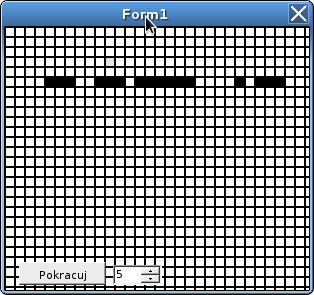
\includegraphics[width=0.7\textwidth]{./img/gol1}
 \label{gol1}
 \caption{The initial state of 'Life' (at t=0)}
\end{figure}

%The evolution of grid for our particular initial state is shown in figure blabla.\\  

Now we press 'Pokracuj' button and let the the Life evolve.

\begin{figure}
 \centering
 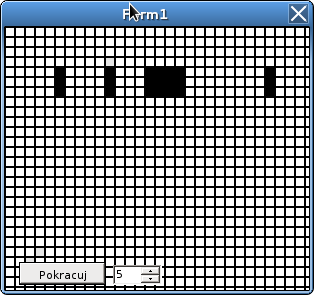
\includegraphics[width=0.7\textwidth]{./img/gol2}
 \label{gol2}
 \caption{t=1}
\end{figure}

\begin{figure}
 \centering
 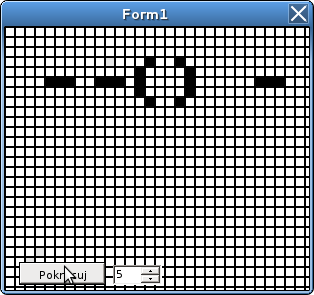
\includegraphics[width=0.7\textwidth]{./img/gol3}
 \label{gol2}
 \caption{t=2}
\end{figure}

In the discrete time steps, the grid is changing.
We see some that cells are dying, but some cells are getting alive. 
What is the rule that kills the cell or leave it be? 
It depends on the state of the cell itself and state of it eight neighbouring cells.
\begin{enumerate}
\item If the cell is alive, and 2 or 3 neighbouring cells are alive, cell will stay alive in the next step, otherwise it will die.
\item If the cell is dead, and EXACTLY 3 neighbouring cells are alive, the cell will get alive in the next step.
\item All other configurations do not change state of the cell.

\end{enumerate}


Let us proceed from this simple example to more general approach.
In the next chapter, we will generalize main features of 'Life' and formally define the cellular automaton.
%In the next chapter, we will generalize main feature of 'Life'
%Let us generalize this example into formal definition of cellular automaton.

\section{Formal definition}
\textbf{Position of cells:}

Instead of 2D rectangular grid from 'Life',
cells might be arranged in arbitrary N dimensional
regular grid, not necessary rectangular. 
(Regularity follows from definition of Kubrid. In general, cells might be positioned really wildly,
e.g. on Penrose lattice, or arbritrary as proposed by Richard P. Feynman).
\bigskip

\textbf{Set of cell states Q:}

In 'Life' cells can be dead or alive (set of states has cardinality 2). 
In general CA, set of states can be any finite set Q of cardinality K.
%cell can be in one of K states from the finiteset of states. 
%We will mark set of states Q, and use this in definition of upgrade rule later.
\bigskip

\textbf{Neighborhood:}

In 'Life', state of the cell in the next step was determined
by 8 neighbouring cells. We call these cells neighborhood of range r = 1 (in the distance of 1 cell).
For general CA, we might consider neighborhood
with arbitrary range.
(Neighborhood with r = 2 in 'Life' would involve 9+16=25 cells).

\bigskip

\textbf{Update rule:}

Update rule is an arbitrary bounded mapping U from Neighborhood to the set of states Q.
Since the state of the Cell is determined only by the state of its Neighborhood, update rules in CA are local.

\section{The most basic cellular automaton} 

In middle 1980s, on the prestigious Princeton institute,
Stephen Wolfram and his assistants were performing unusual computer experiments \cite{levy} and analyzing the patterns by 1D cellular automata (to a despair of their senior colleagues)\cite{levy}.

The most basic CA is 1D CA with range r=1 and its cells can be in one of two states (alive or dead).

1D CA means, that cells are arranged in the row, see Fig.~\ref{1d}

\begin{figure}[htbp]
 \centering 
 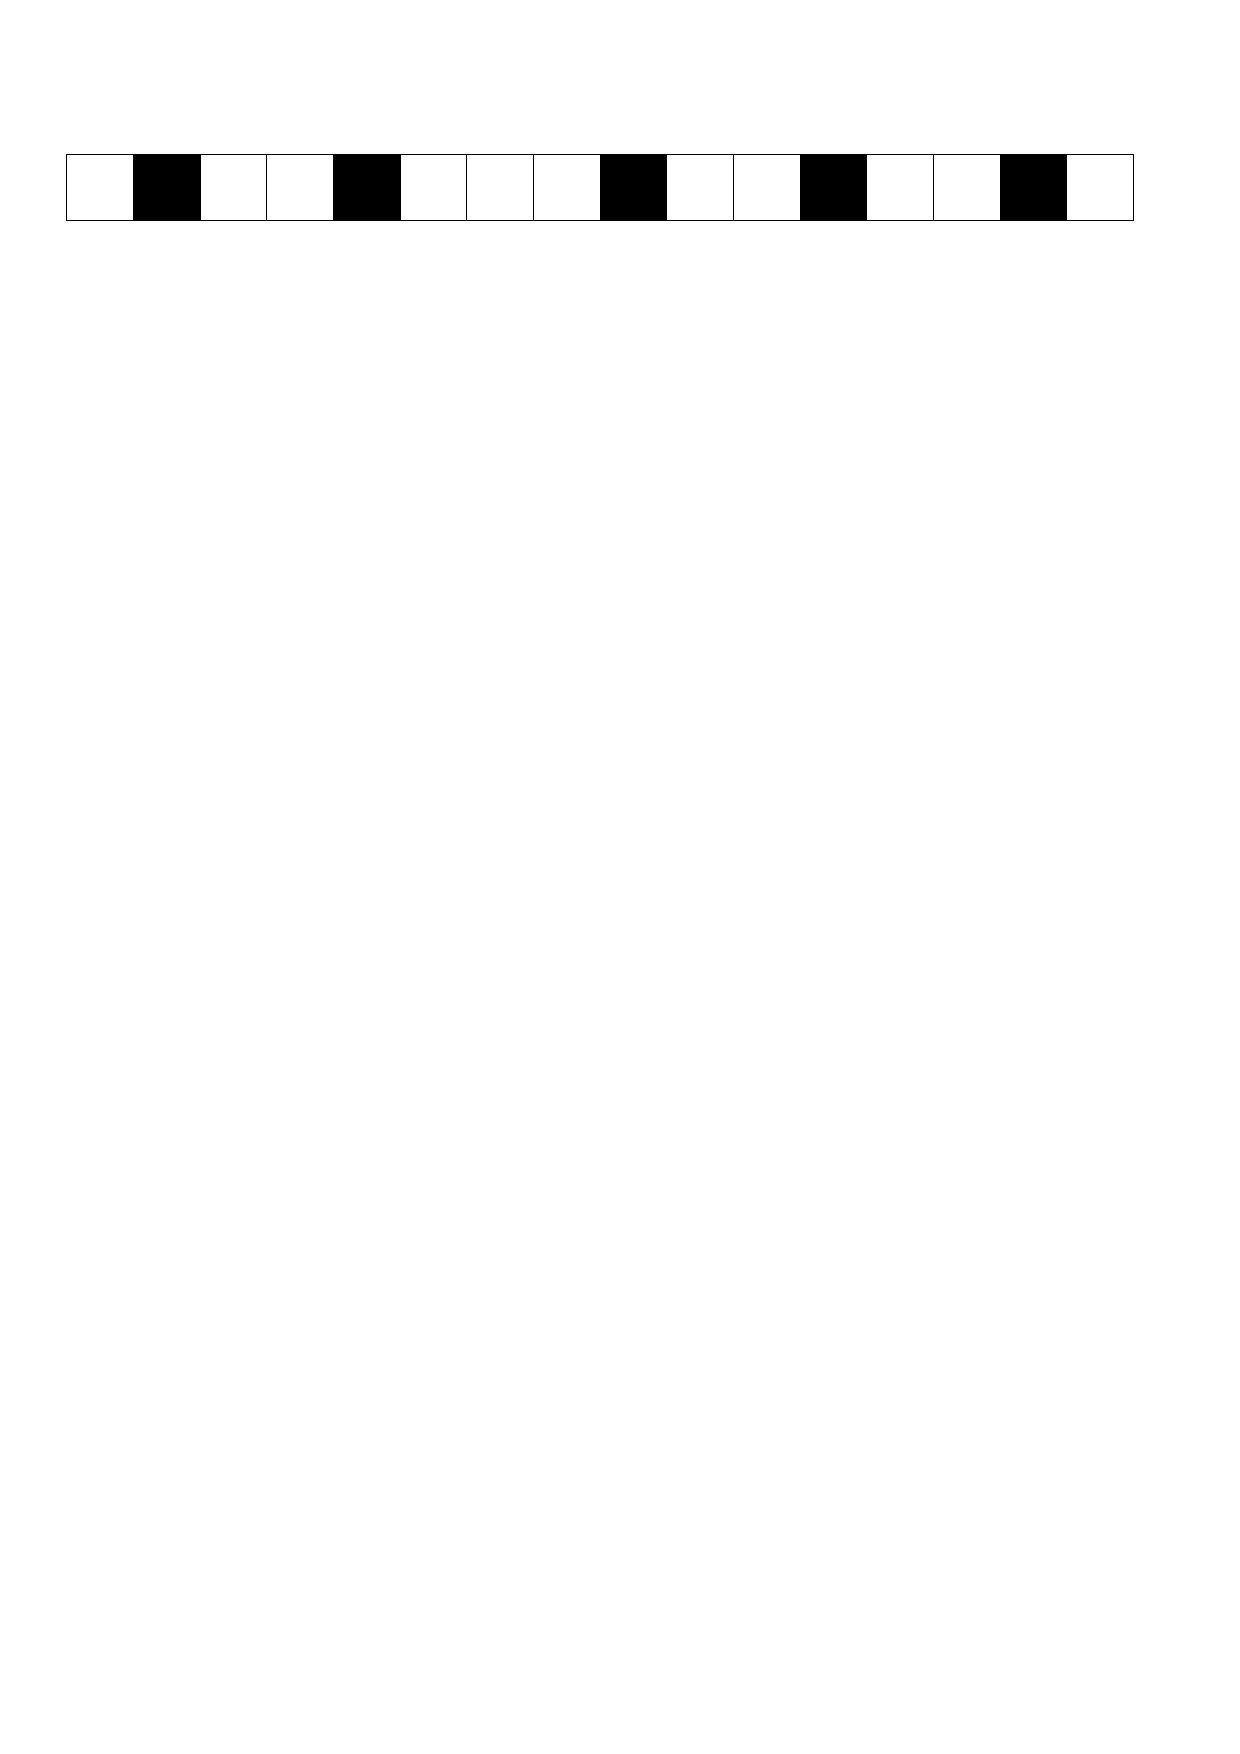
\includegraphics[width=0.9\textwidth]{./img/1Dline}
 \label{1d}
 \caption{1D cellular automaton}
\end{figure}

Range r=1 means that in update rule, 
we consider states of 3 cells. The cell itself, 
1 neighbour to the left and 1 to the right.\\

Example of an update rule is in the Table~\ref{rule90}.\\


\begin{table}[htbp]
 \centering
 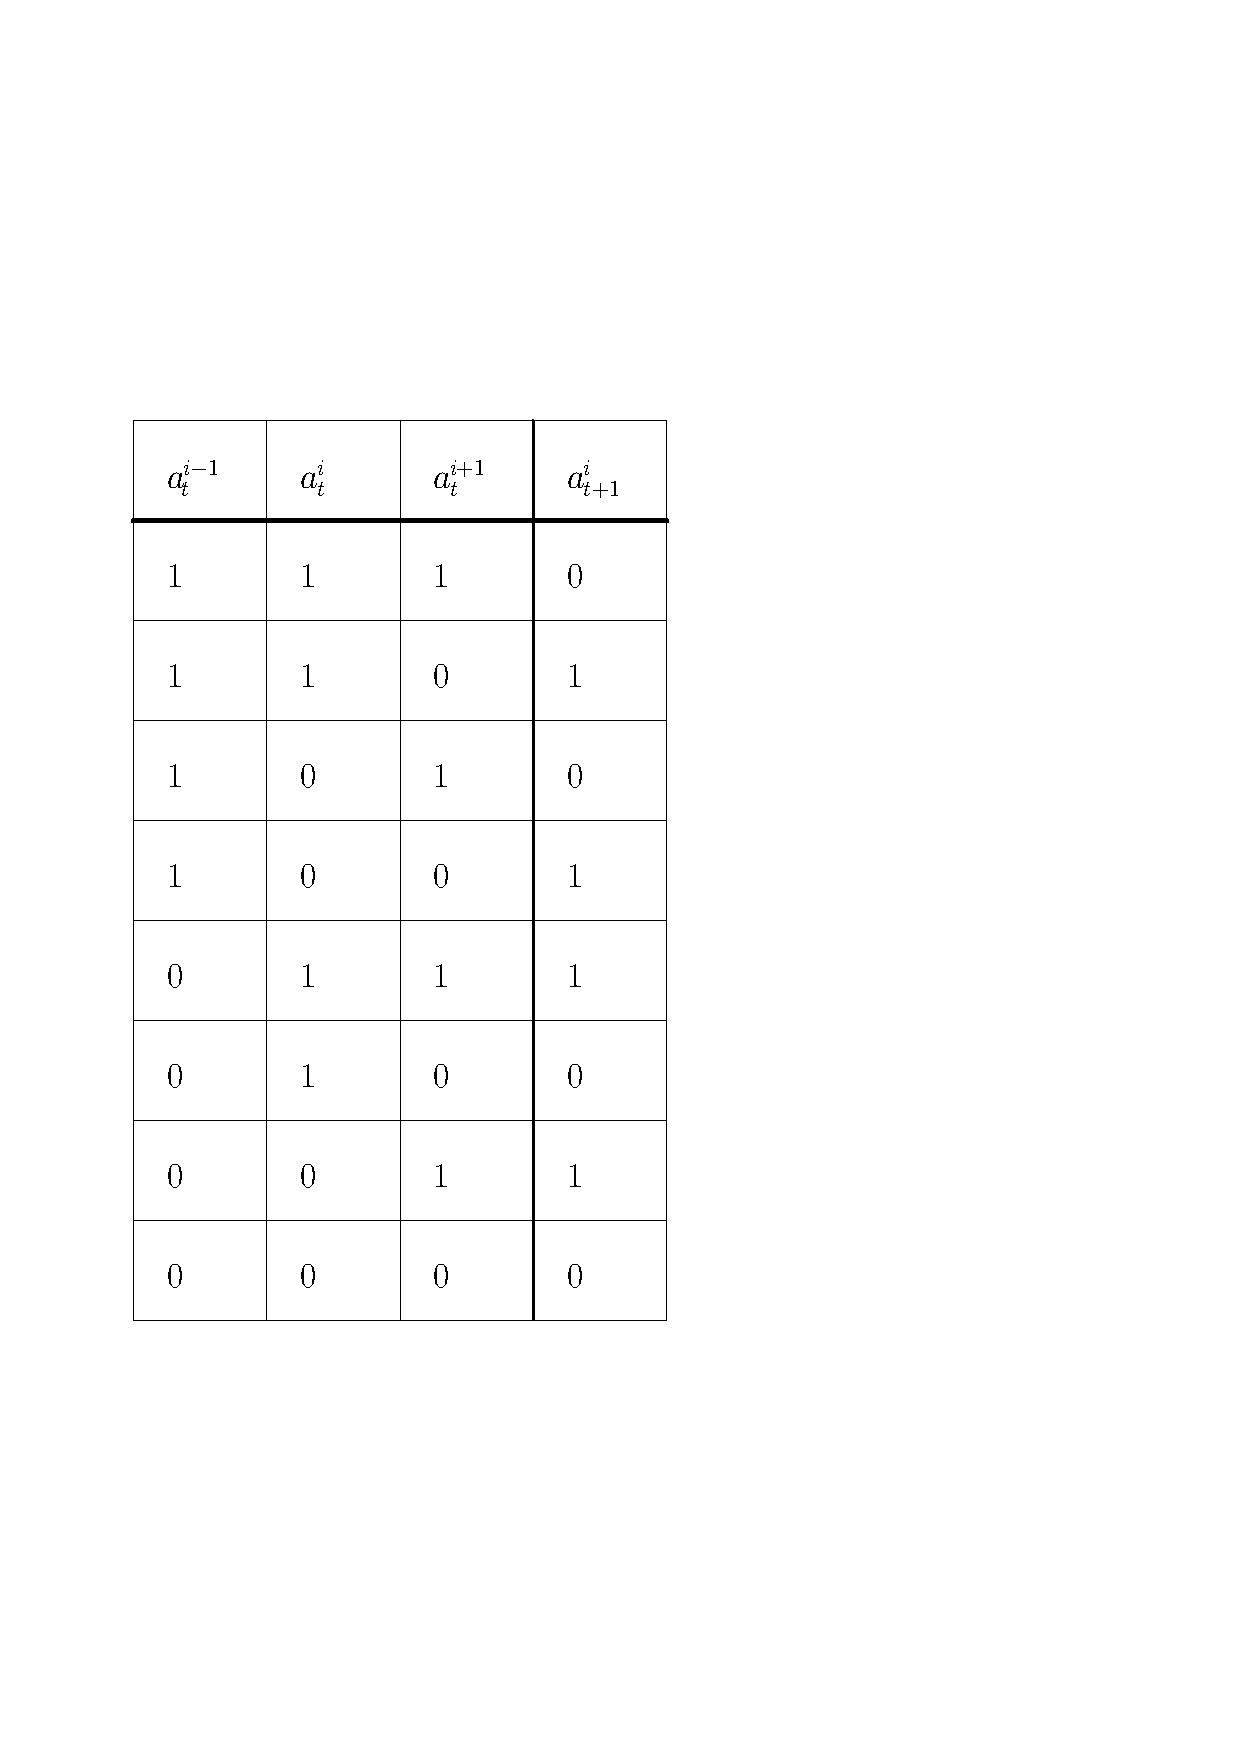
\includegraphics[width=0.4\textwidth]{./img/1Drule}
 \caption{Rule 90}
 \label{rule90}
\end{table}

%How many different update rules ("how many different Tables~\ref{rule90}")
%exist for this type of CA?

First three columns of the table denotes state of the three cells, $a_t^i$ is the middle cell and the other two are its left and right neighbor.

The rule specifies the state of the middle cell after update, based on the configuration of these three cells.
The number of possible configurations of the three cells is $2^3 = 8$.
So the rule must specify 8 bits (for each configuration one bit).
It means there are $2^8 = 256$ different rules for this most basic cellular automaton.

Let us take a look at some pictures of these cellular automata. These pictures were ploted by the simple program that we programmed for this purpose.

These pictures represent the sequences of states of cellular automata with rules 90, 30, 45 and 73.
The downer-most row is the initial configuration of CA, 
the 2nd row is configuration after 1st update etc.

\begin{figure}
 \centering
 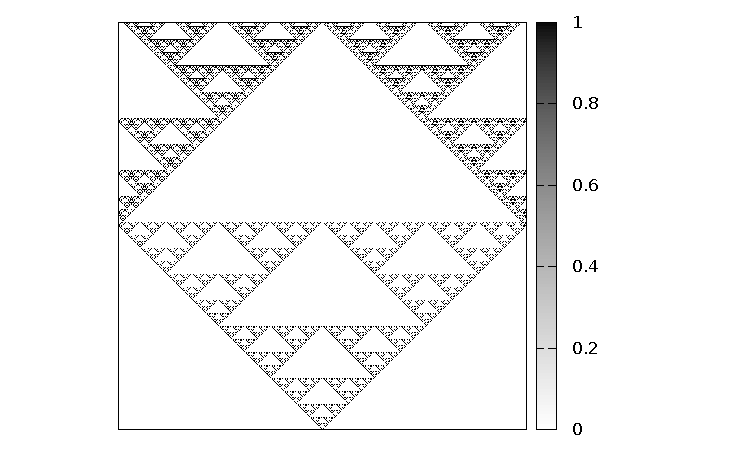
\includegraphics[width=1\textwidth]{./img/rule90}
 \caption{Rule 90}
 \label{koberec}
\end{figure}

\begin{figure}
 \centering
 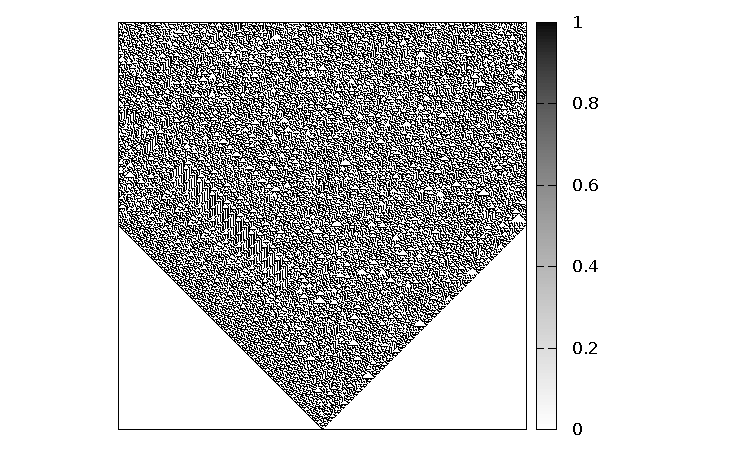
\includegraphics[width=1\textwidth]{./img/rule30}
 \caption{Rule 30}
\end{figure}

\begin{figure}
 \centering
 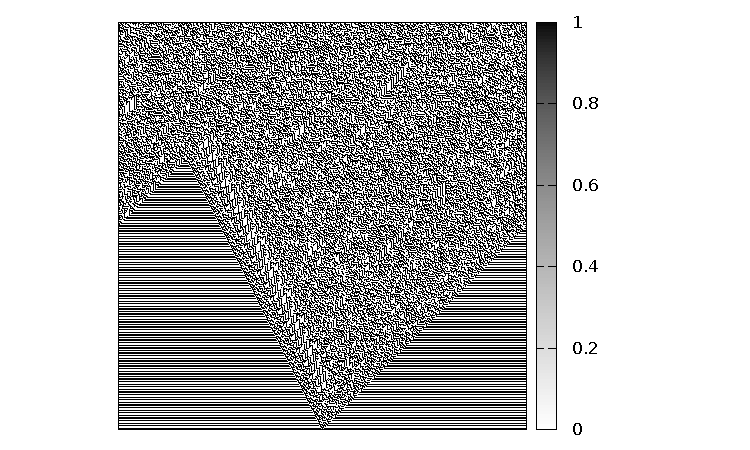
\includegraphics[width=1\textwidth]{./img/rule45}
 \caption{Rule 45}
\end{figure}

\begin{figure}
 \centering
 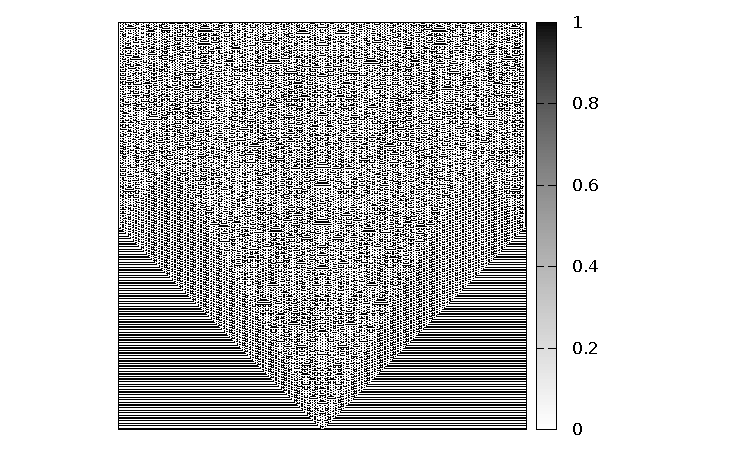
\includegraphics[width=1\textwidth]{./img/rule73}
 \caption{Rule 73}
\end{figure}

First picture~\ref{koberec} is famous fractal known as Sierpinski carpet. Wolfram classified these 1D automata into four classes, based on the regularity of the pattern obtained.

Wolfram argues that variety of behavior seen even in these most simple CA rises suspitions, and encourage hope, that in the infinitely large world of possible CAs, there is CA that model any complex phenomena you can imagine.

In his visionary book New kind of Science, Wolfram even proposes Cellular automaton that would constitute a unified theory of the fundamental physics.
Although his ideas met with rejection among theorists (see \cite{aaronson}),
many other notable physicists are attempting to construct such cellular automaton \cite{hooft}).

Some of the basic construction principles for such automata are relevant also for our models, but mostly, we would diverge too far by further exploration.
Focus of our work is much more modest that CAs describing universe.
Our focus is on CAs that model flows of the fluids.

The connection of the cellular automata with flow of fluids is not obvious or formal.
It is found on the very general level.
What connects Navier-Stokes equations and CAs are their common symettries and conservation laws implied by these symetries.
In these symmetries lies not only beauty of this method, but their strongest advantage over other well-established CFD methods.
\chapter{Lattice gass cellular automata}
The first lattice gass cellular automaton was proposed in 1973 by Hardy, Pomeau and de Pazis, and it is called -- the HPP model.

Unfortunately, it could not do its job sufficiently well. For the reasons that we will sketch in this chapter, it does not converge to Navier-Stokes equations in macroscopic limit.

\bigskip

In the subsequent chapters we will explore two different approaches how to make functional LGCA. They both build on the idea of this imperfect HPP.

Therefore, we will explain the basic principles of HPP first, and later on, we will upgrade it - either to FHP, Pair-interaction or their multi-dimensional variants.

\section{From CA to LGCA}

The lattice of HPP is the simple rectangular 2D grid. At every point of a grid is a node, and this node is composed of 4 cells, see Figure~\ref{rectangular}.

\begin{figure}[htbp]
 \centering
 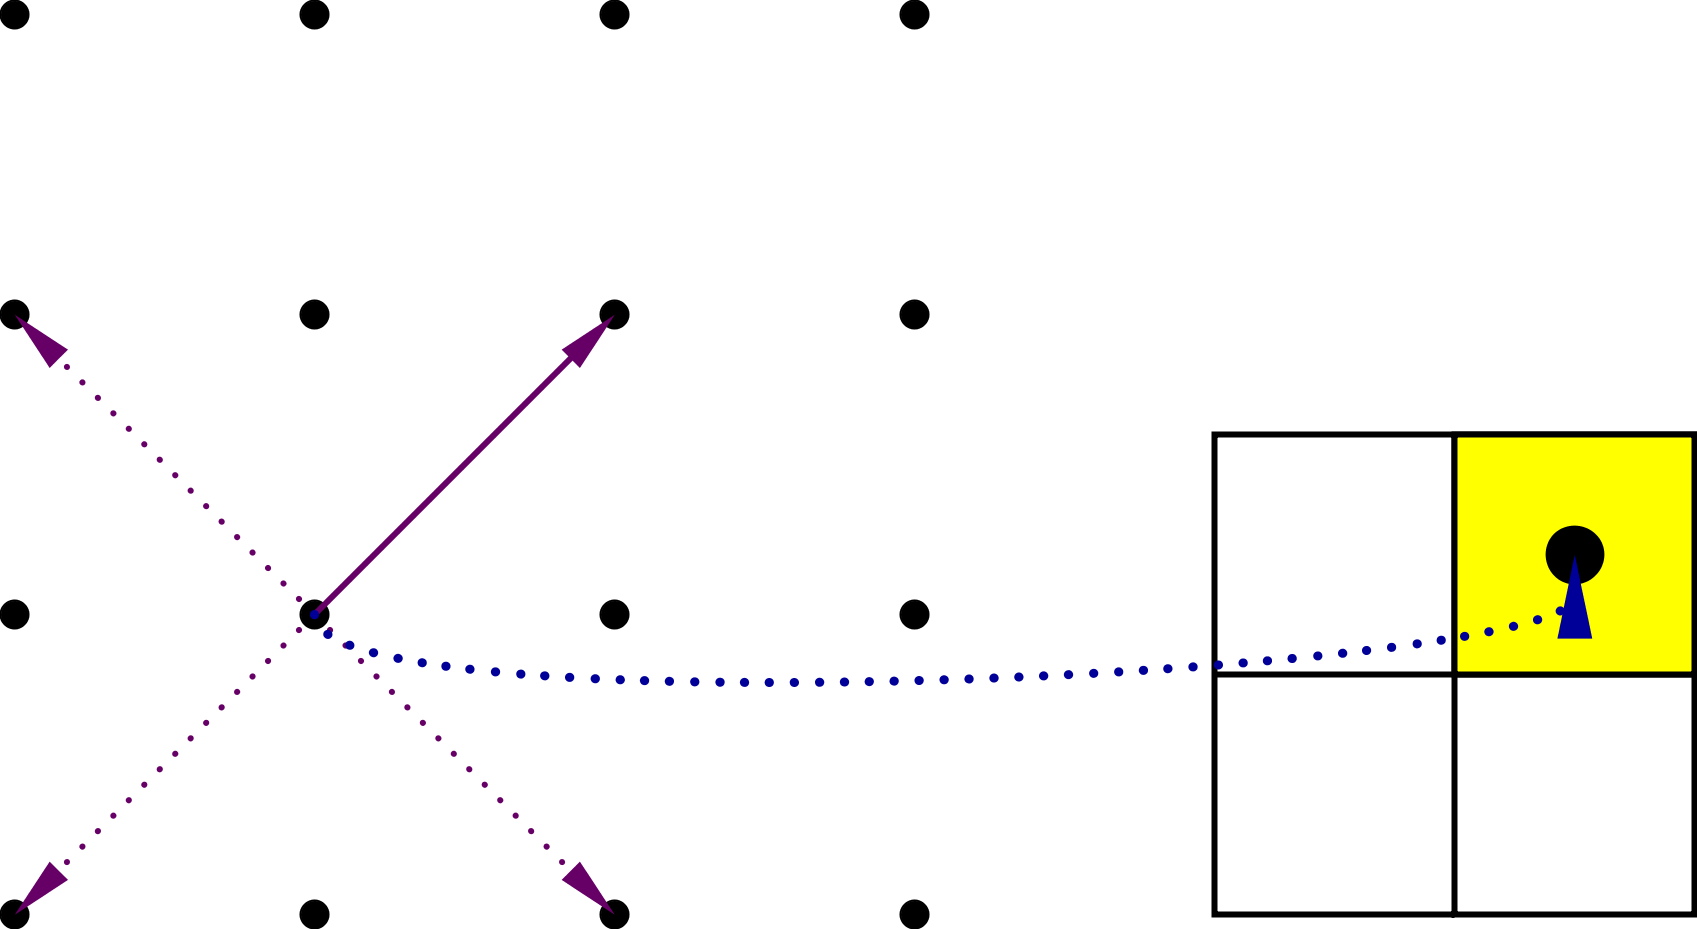
\includegraphics[width=0.6\textwidth]{./img/hppnode}
 \label{rectangular}
 \caption{Rectangular grid}
\end{figure}

Each of these cells can be in two states-- empty (white square) or occupied by the particle (yellow square).
The particle in this cell is heading to the diagonal node along the corresponding lattice vector.

\section{Update rule}
%The update rule should be design in such a manner, that is conserve physically relevant quantities, namely mass and momentum.

Every time-step, the position of the particles is changing. The update is done in two subsequent steps -- collision and propagation.

In the collision step, particles are swapped inside the single node, respecting two constraints - number of particle is same after the collision, and the total momentum in the node is same.

From these constraints follows that in HPP, there are only two collision configurations, see Figure~\ref{hpp-colision}.

\begin{figure}[H]
 \centering
 \includegraphics[width=0.7\textwidth]{./img/hpp_col}
 \label{hpp-colision}
 \caption{HPP colisions}
\end{figure}

These collision configurations are symmetric -- the first configuration is resolved to the other and vice versa.

It is easy to understand that there are no other collision configurations and collision rules. If any other state gets changed, it would break the conservation of momentum and would be physically unrealistic.

\section{Propagation:}

After the collisions are resolved in every node, propagation follows -- figure \ref{hpp-prop}.
During propagation, the particle moves from node to node, along the lattice vectors that corresponds to the cells they occupied.
\begin{figure} [H]
 \centering
 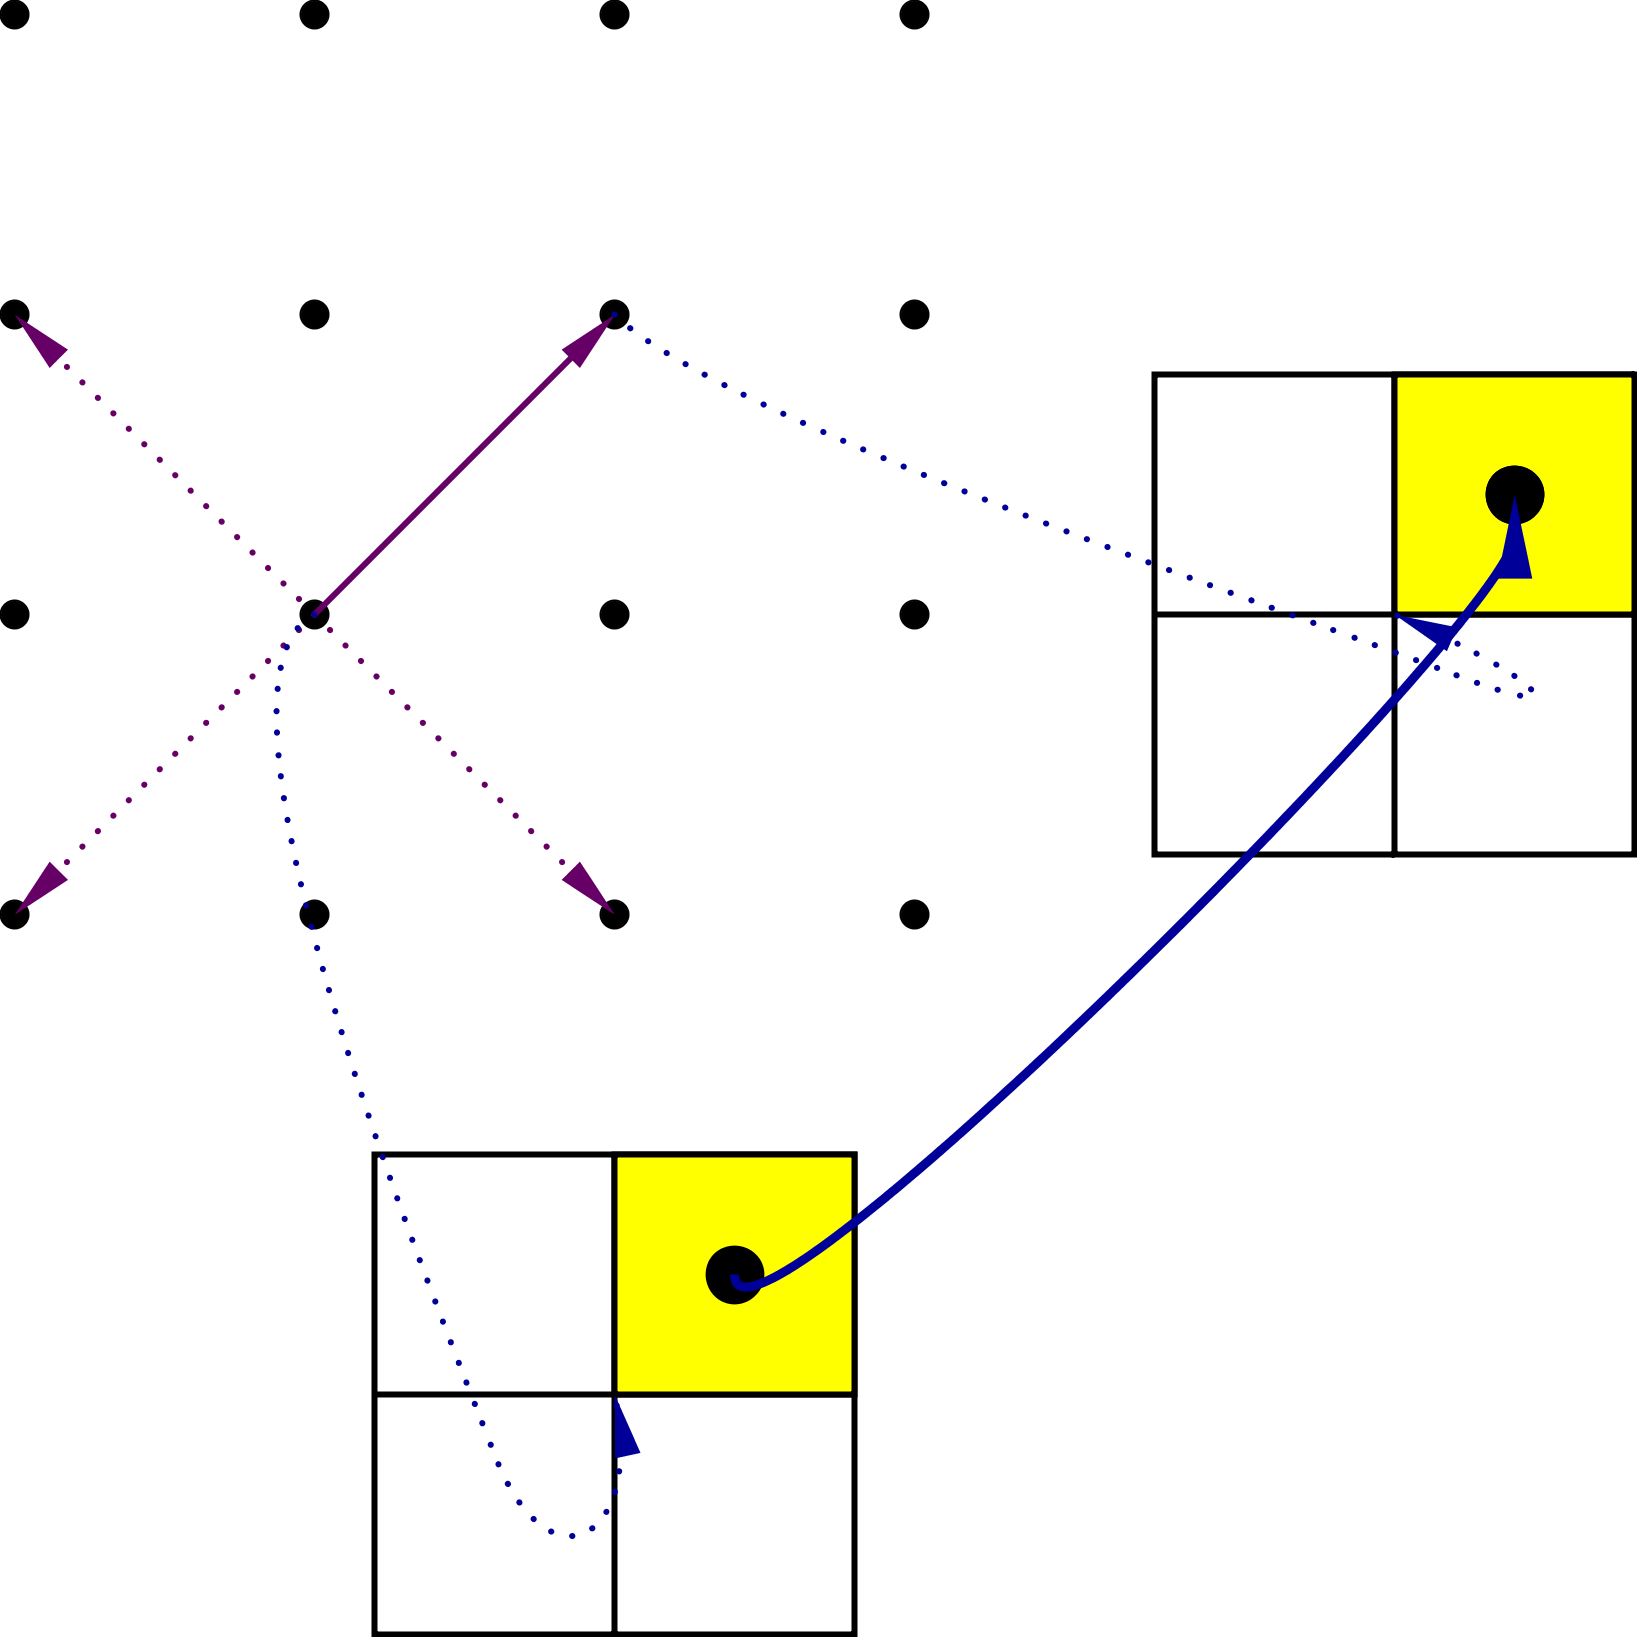
\includegraphics[width=0.6\textwidth]{./img/HPPprop}
 \label{hpp-prop}
 \caption{Propagation of particle from upper-left cell}
\end{figure}

\bigskip

\section{Conservation laws}

We already noted that collision and propagation conserve momentum, and they obviously conserve mass, since particles are neither created, nor anihilated during update. 
Let us inspect these conservation laws in the more depth by considering symmetries of this model.

Suppose we have lattice of infinite size (or finite size, but periodic boundary condition are used). Then if we shift the lattice by multiple of lattice vector, we get the same lattice -- the lattice is symmetric with respect to translation.
As we know by Norther's theorems, translational symmetry implies conservation of momentum.

\bigskip

Also, the grid possesses a rough rotational symmetry - rotation by the $90\degree$ leads to the same lattice.

However, this rectangular symmetry is not sufficient.
When we derive the hydrodynamic equations in the following chapter, we will observe that four lattice vectors lead to unrealistic equations, comparing to the models with six and more lattice vectors.

\bigskip
Another problem caused by low rotational symmetry are the non-physical quantities that are conserved nevertheless -- so called spurious invariants \footnote{The improved LGCA also posses the spurious \textit{Zanetti's invariants}, but they are under level of noise, due to higher symmetry or additional degrees of freedom in the node}.

Consider the total momentum in the node before and after collision on the figure \ref{hpp-colision}.
Let us decompose the total momentum into the cardinal directions:
\begin{align} 
P = P_N + P_S + P_E + P_W.
\end{align}
This total momentum $P$ is correctly conserved by HPP collison, but also quantities
\begin{align} \label{zanet}
P_{spur1} = P_N + P_E - P_S - P_W
\end{align}
and
\begin{align}
P_{spur2} = P_N + P_W - P_S - P_E
\end{align}
are conserved, although these quantities have no physical counterparts.

\bigskip

To conclude this chapter and finish-off the HPP, it is physically implausible because
\begin{enumerate}
\item angular momentum is not conserved due to insufficient rotational symmetry,
\item other non-physical quantities, so called \textit{spurious invariants} are conserved.
\end{enumerate}

Although it is a flawed model, it sparked interest of the wider community and various successful LGCAs evolved from HPP. In the next chapter, we will introduce the first physically relevant branch of LGCAs -- the FHP model.
\chapter{FHP}
This improved lattice gas cellular automaton is named after its inventors too -- Frisch, Humpfrey and Pomeu. 
They proposed it in 1986 together with its three dimensional variant - the FCHC. 

In following section, we will graphically explain the basic principles of FHP, the other sections will be more general and the obtained results will be valid for arbitrary dimensional FHP-like automaton (most importantly FCHC).

\section{The lattice of FHP}
All the improvements of FHP are result of one simple change - instead of square grid, FHP builds on hexagonal grid. 

The two dimensional plane can be uniformly covered by squares, but also by hexagon, that . This is the main improvement of FHP, all other properties are implied by the properties of the hexagonal grid.

On the Figure \ref{FHPgrid}, we see part of this hexagonal lattice. The dots represent the nodes.
On the figure \ref{FHPgrid}, we have a part of hexagonal grid, and from one of the node, six lattice vectors points to the neighboring nodes.
\begin{figure}[htbp] \label{FHPgrid}
 \centering
 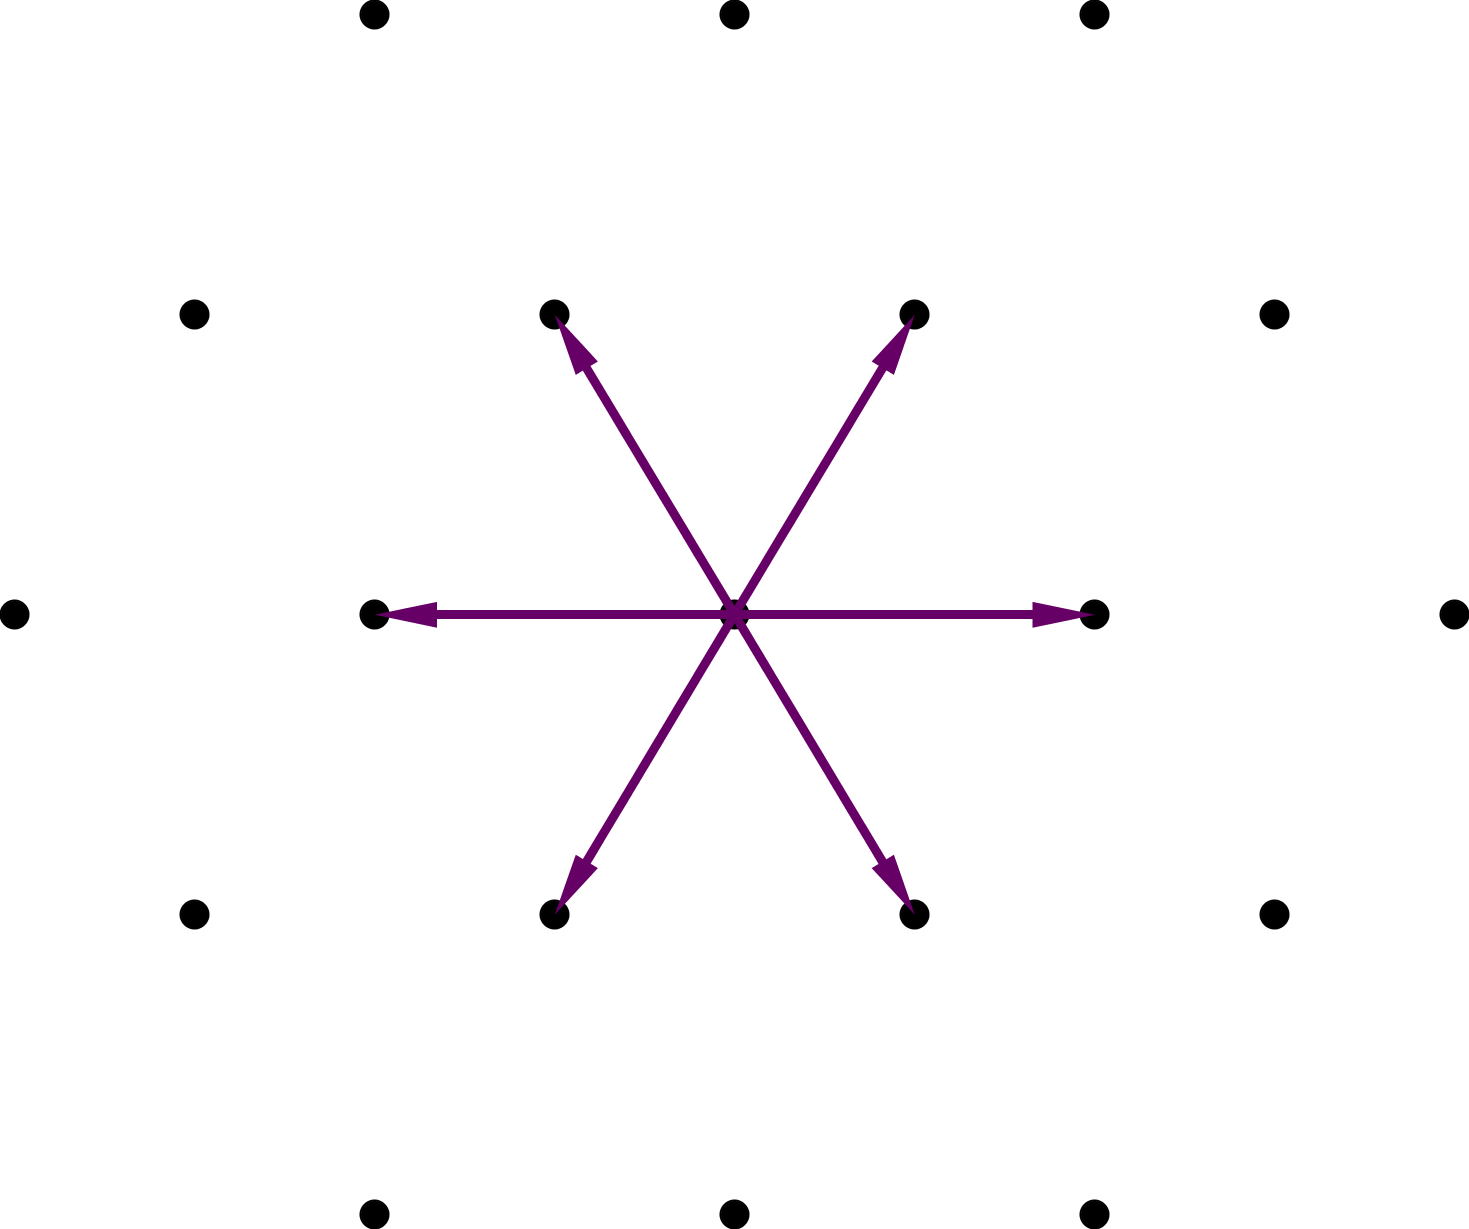
\includegraphics[width=0.6\textwidth]{./img/fhp_desc}
\end{figure}

Therefore, every node consists of the six cells corresponding to these six lattice vectors. Each of these cells can be occupied by a particle, and we identify velocities of the particles with the lattice vectors.

\section{Update rule}
In all the LGCAs that we will present, update of the lattice consists of two subsequent steps - collision and propagation.

The role of the collision is to change the state of the node as much as possible, so that viscosity is minimized.
The only constraint on the collision rule is to preserve the number of particles (conservation of mass) and to preserve the total momentum in the node (conservation of momentum).

These requirements lead only to a handful of collision configurations, see figure \ref{FHPcol}. For the simplicity, we are considering the FHP-I model, that does not included the "rest particles", otherwise we would have to include few more collisions.

\begin{figure}[H]
 \centering
 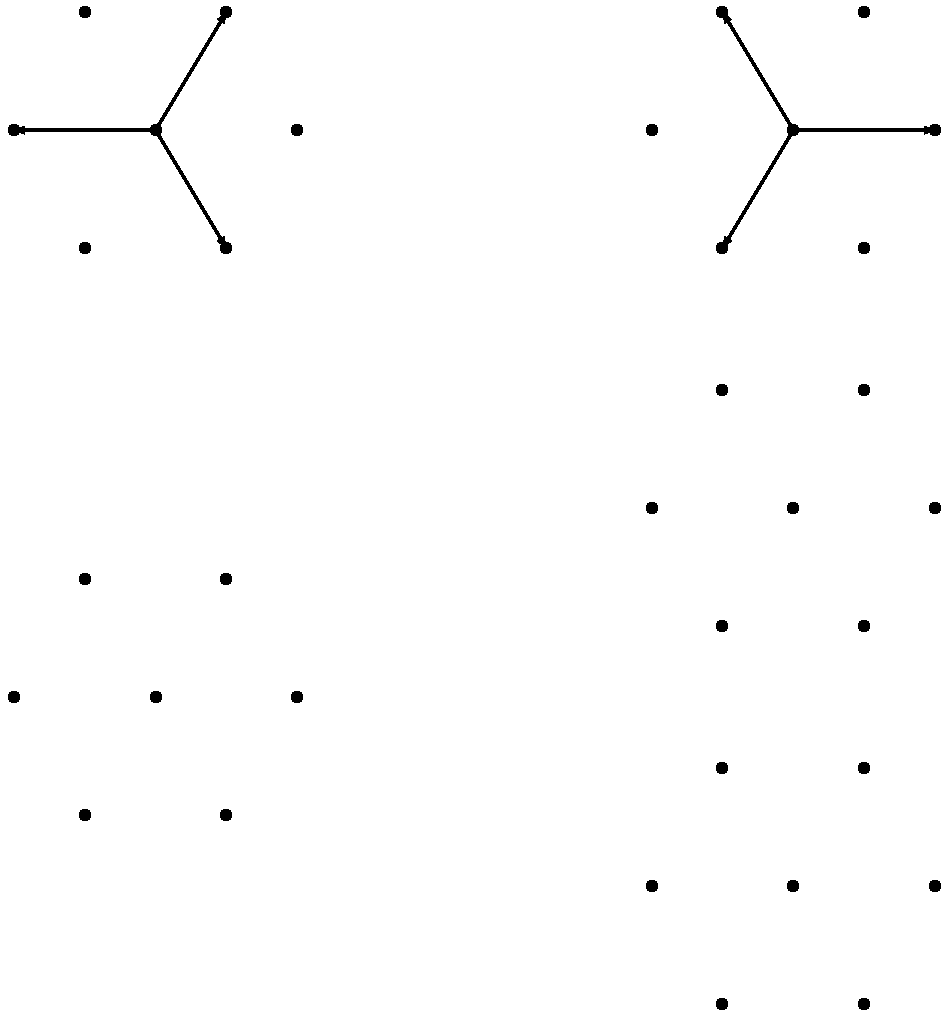
\includegraphics[width=0.7\textwidth]{./img/FHPcol}
 \caption{FHP collisions without rest particle.}
 \label{FHPcol}
\end{figure}

We see that two and four particle configurations can be resolved in two different configurations. The resulting state need to be chosen randomly, with probability $1/2$ for each state (if there was a preferred configuration, the model would posses a non-physical invariant -- chirality).

When the collision is resolved in every node, propagation follows.
This phase is straigt-forward -- if the cell is occupied by a particle, it propagates along the corresponding lattice vector to the neighboring node, see figure \ref{FHPprop}.


\begin{figure}[H]
 \centering
 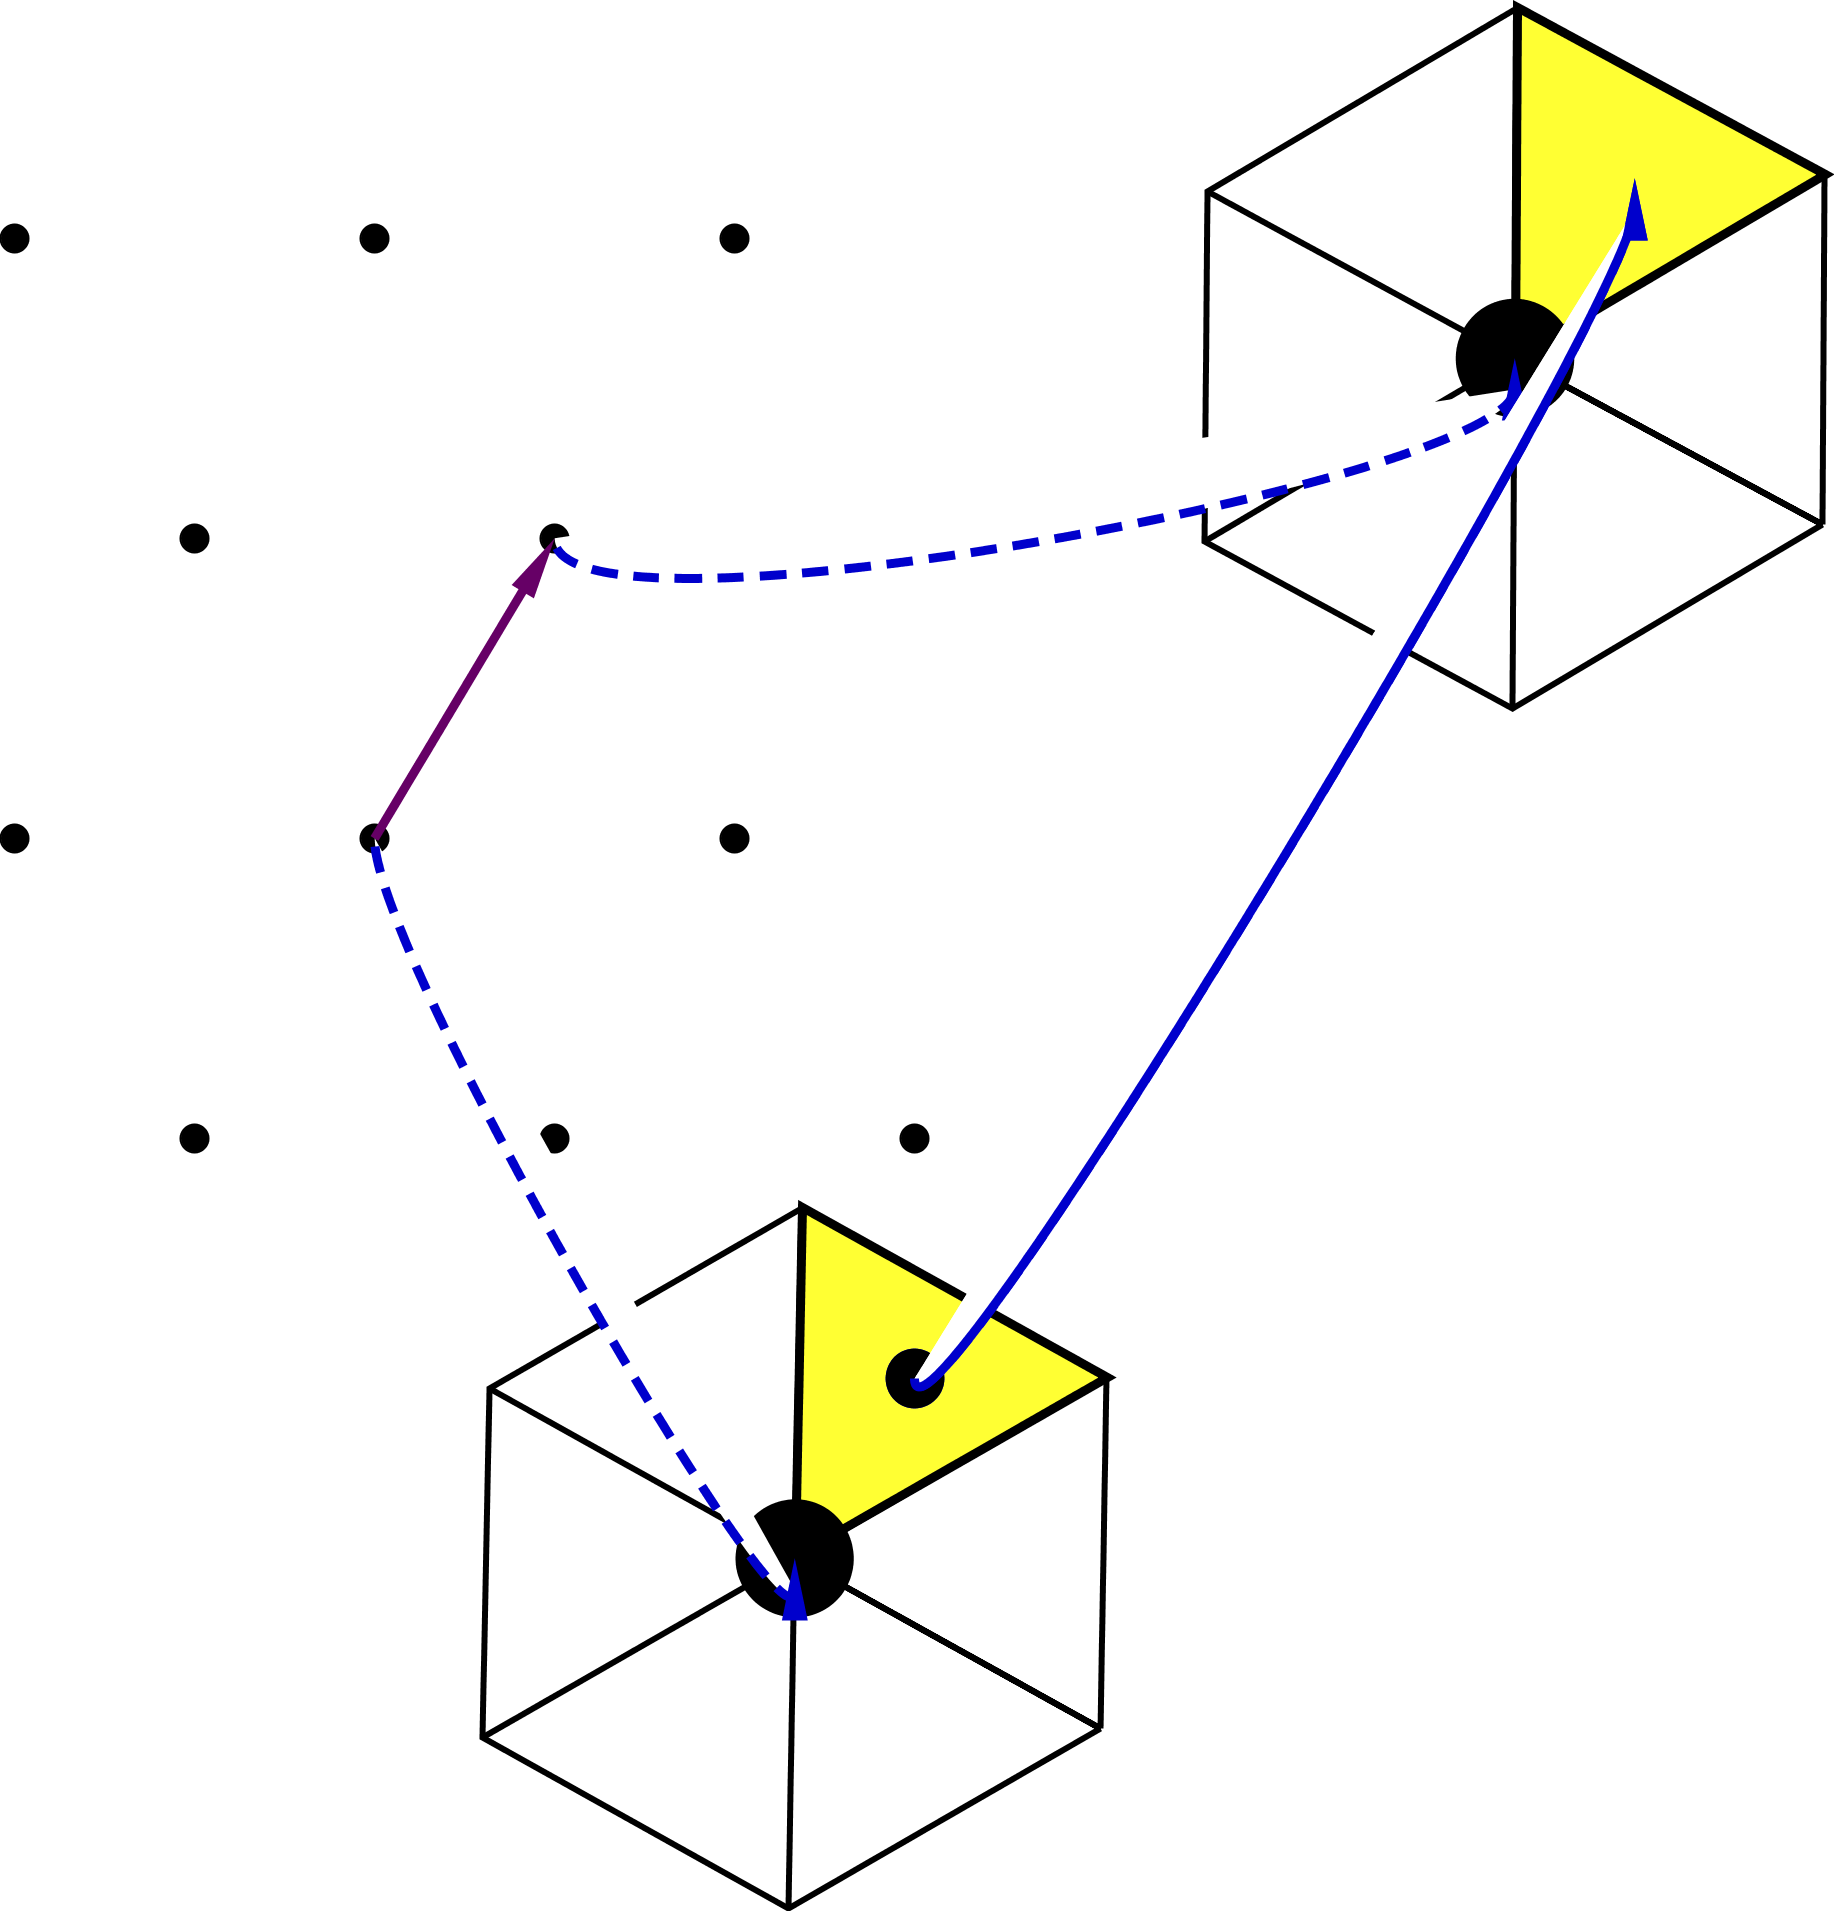
\includegraphics[width=0.7\textwidth]{./img/FHPprop}
 \caption{FHP collisions without rest particle.}
 \label{FHPprop}
\end{figure}

Comparing it to HPP, we have a mesh with better rotational symmetry and nodes with richer  set of collisions.

Now that we presented the setting of FHP in two dimensions, let us explore the microdynamics of FHP in more formal way. This formal treatment enables us to derive the hydrodynamic equations for FHP-like automata in arbitrary dimension (although finding an appropriate multidimensional lattice is non-trivial and possible only in 4 dimensions, as we will see).


Although we will form 
In the previous chapters, we seen how FHP and HPP works in intuitive way. 
In this chapter, we will treat this automata more analytically, hence we need to get more formal.

We will try to make this chapter more general, so that the obtained statistical limit is applicable for all cellular automata from the same class as FHP - specifically its predecessor HPP and its 3D upgrade FCHC.

\bigskip

But since we already have concrete idea of how FHP works, it will be the good point to start.

\section{FHP analytically}

Now that we have good intuition about FHP model, we need to get more formal to treat LGCA analytically.

State of the node will be denoted by $n = (n_1,n_2,n_3,n_4,n_5,n_6)$, where $n_i = 0$ means that $i^{th}$ cell in the node is empty, and $n_i = 1$ means that there is particle in the $i^{th}$ cell.

State of the \textbf{specific node} (at the position \textbf{r} on the lattice) will be denoted by $\bf{n(r)}$, whereas state of \textbf{all the nodes} in the lattice will be denoted by \textbf{n(.)}.

We already know that update of the whole lattice is local, hence we can treat it node by node.

We also know that update happens in discrete time steps, and it can be divided into two sub-steps - collision, and propagation.

\section{Propagation}
Propagation is straight-forward for all types of LGCA and can be captured by very simple equation
\begin{equation}
S n_i(\bf{r}) = n_i(\bf{r + c_i}). 
\end{equation}
This equation means that state of the $i^{th}$ cell in node \textbf{n(r)} propagates along the lattice vector $c_i$ to the neighboring node $\bf{n(r + c_i)}$, see figure below.\\
\\
To put it in the nutshell, propagation is completely determined by the geometry of the lattice. Once we know what the lattice vectors $c_i$ are, we know all about propagation (equation blabla).\\
\\
Where the dark magic of LGCAs hides is the collision step.\\

\section{Collision}
The purpose of collision is to change the configuration of the node as much as possible (it means to change as many bits of the node as possible), while we preserve mass and momentum.\\
(if we change direction of the particle). 

For HPP, we have only $2^4 = 16$ possible states in node, and only two collision configurations among them. Since these configurations are symmetric, we have only one collision rule.\\
For FHP, we have $2^6 = 64$ configurations, and whole bunch of collision configurations among them, but we can still draw the simple picture of these configurations:\\
\\
As we see, head-on 2-particle collisions can result in two different states. If we wanted to preserve determinism, and we were systematically choosing only one of them, we would introduce additional, non-physical invariance - the model would become chiral. If we want to preserve the parity symmetry of the model, we need to assign equal probability to either of two final states.Hence, we are introducing non-determinism to the model.

We will express the probabilities of transition from state $n$ to state $n'$ by probability matrix:
\begin{equation}
A(n \rightarrow n') \geq 0
\end{equation}
As we have 64 possible states of the node, matrix A is of dimension $64\times 64$.
For example, the cell of matrix A that governs the head-on collisions looks like this:
\[
 A'=
  \begin{bmatrix}
    0 & \frac{1}{2} & \frac{1}{2} \\
    \frac{1}{2} & 0 & \frac{1}{2} \\
    \frac{1}{2} & \frac{1}{2} & 0 \\
  \end{bmatrix}
\]
Since the collisions are symmetric, matrix A is symmetric as well.

Also, collisions are invariant to rotations or reflections of the node:
\begin{equation}
A(g(n) \rightarrow g(n')) = A(n \rightarrow n')
\end{equation}
where $g \in G$, and G is the symmetry group of the node.

\section{Collision operator}
Interestingly, we can express the whole update step in one simple equation using collision operator $\Delta_i$:
\begin{equation}
n_i(t+1,r+c_i) = n_i(t,r) + \Delta_i(t,r)
\end{equation}
If this equation works, then, $\Delta_i$ must be:
\begin{enumerate}
\item $\Delta_i = 0$ if no collision is happening in $n(t,r)$. Then state of the cell $n_i(t,r)$ only propagates to $n_i(t+1,r+c_i)$.
\item $\Delta_i = 1$ if there is not particle in $n_i(t,r)$ yet, but gets there after collision. 
 \item $\Delta_i = -1$ if there is particle in the $n_i(t,r)$, but after collision, cell gets empty.
\end{enumerate}

\bigskip

For example, $\Delta_i$ acquire very simple form for HPP:
\begin{equation}
\Delta_i = n_{i+1} n_{i+3}( 1 - n_i)(1 - n_{i+2}) - n_i n_{i+2}(1-n_{i+1})(1 - n_{i+3})
\end{equation}
As there are only 2 collision configuration in HPP, $\Delta_i$ has 2 terms.
If either collision happens, corresponding term is 1.

\section{Microscopic conservation laws}
Using collision operator, conservation of mass and momentum is this simple:
\begin{subequations}
\begin{align}
\sum_i \Delta_i(t,r) &= 0,\\
%
\sum_i c_i \Delta_i(t,r) &= 0
\end{align}
\end{subequations}
(Prove: unfold $\Delta$s)
Conservation laws can be equivalently expressed in the form
\begin{align} \label{cons1}
\begin{split}
\sum_i n_i(t+1, r + c_i) &= \sum_i n_i(t,r), \\
\sum_i c_i n_i(t+1, r + c_i) &= \sum_i c_i n_i(t,r).
\end{split}
\end{align}
%\chapter{Microdynamics of FHP}

Although we will form 
In the previous chapters, we seen how FHP and HPP works in intuitive way. 
In this chapter, we will treat this automata more analytically, hence we need to get more formal.

We will try to make this chapter more general, so that the obtained statistical limit is applicable for all cellular automata from the same class as FHP - specifically its predecessor HPP and its 3D upgrade FCHC.

\bigskip

But since we already have concrete idea of how FHP works, it will be the good point to start.

\section{FHP analytically}

Now that we have good intuition about FHP model, we need to get more formal to treat LGCA analytically.\\
\\
State of the node will be denoted by $n = (n_1,n_2,n_3,n_4,n_5,n_6)$, where $n_i = 0$ means that $i^{th}$ cell in the node is empty, and $n_i = 1$ means that there is particle in the $i^{th}$ cell.\\
\\
State of the \textbf{specific node} (at the position \textbf{r} on the lattice) will be denoted by $\bf{n(r)}$, whereas state of \textbf{all the nodes} in the lattice will be denoted by \textbf{n(.)}.\\
\\
We already know that update of the whole lattice is local, hence we can treat it node by node.\\
We also know that update happens in discrete time steps, and it can be divided into two sub-steps - collision, and propagation.

\section{Propagation}
Propagation is straight-forward for all types of LGCA and can be captured by very simple equation
\begin{equation}
S n_i(\bf{r}) = n_i(\bf{r + c_i}). 
\end{equation}
This equation means that state of the $i^{th}$ cell in node \textbf{n(r)} propagates along the lattice vector $c_i$ to the neighboring node $\bf{n(r + c_i)}$, see figure below.\\
\\
To put it in the nutshell, propagation is completely determined by the geometry of the lattice. Once we know what the lattice vectors $c_i$ are, we know all about propagation (equation blabla).\\
\\
Where the dark magic of LGCAs hides is the collision step.\\

\section{Collision}
The purpose of collision is to change the configuration of the node as much as possible (it means to change as many bits of the node as possible), while we preserve mass and momentum.\\
(if we change direction of the particle). 

For HPP, we have only $2^4 = 16$ possible states in node, and only two collision configurations among them. Since these configurations are symmetric, we have only one collision rule.\\
For FHP, we have $2^6 = 64$ configurations, and whole bunch of collision configurations among them, but we can still draw the simple picture of these configurations:\\
\\
As we see, head-on 2-particle collisions can result in two different states. If we wanted to preserve determinism, and we were systematically choosing only one of them, we would introduce additional, non-physical invariance - the model would become chiral. If we want to preserve the parity symmetry of the model, we need to assign equal probability to either of two final states.Hence, we are introducing non-determinism to the model.

We will express the probabilities of transition from state $n$ to state $n'$ by probability matrix:
\begin{equation}
A(n \rightarrow n') \geq 0
\end{equation}
As we have 64 possible states of the node, matrix A is of dimension $64\times 64$.
For example, the cell of matrix A that governs the head-on collisions looks like this:
\[
 A'=
  \begin{bmatrix}
    0 & \frac{1}{2} & \frac{1}{2} \\
    \frac{1}{2} & 0 & \frac{1}{2} \\
    \frac{1}{2} & \frac{1}{2} & 0 \\
  \end{bmatrix}
\]
Since the collisions are symmetric, matrix A is symmetric as well.

Also, collisions are invariant to rotations or reflections of the node:
\begin{equation}
A(g(n) \rightarrow g(n')) = A(n \rightarrow n')
\end{equation}
where $g \in G$, and G is the symmetry group of the node.

\section{Collision operator}
Interestingly, we can express the whole update step in one simple equation using collision operator $\Delta_i$:
\begin{equation}
n_i(t+1,r+c_i) = n_i(t,r) + \Delta_i(t,r)
\end{equation}
If this equation works, then, $\Delta_i$ must be:
\begin{enumerate}
\item $\Delta_i = 0$ if no collision is happening in $n(t,r)$. Then state of the cell $n_i(t,r)$ only propagates to $n_i(t+1,r+c_i)$.
\item $\Delta_i = 1$ if there is not particle in $n_i(t,r)$ yet, but gets there after collision. 
 \item $\Delta_i = -1$ if there is particle in the $n_i(t,r)$, but after collision, cell gets empty.
\end{enumerate}

\bigskip

For example, $\Delta_i$ acquire very simple form for HPP:
\begin{equation}
\Delta_i = n_{i+1} n_{i+3}( 1 - n_i)(1 - n_{i+2}) - n_i n_{i+2}(1-n_{i+1})(1 - n_{i+3})
\end{equation}
As there are only 2 collision configuration in HPP, $\Delta_i$ has 2 terms.
If either collision happens, corresponding term is 1.

\section{Microscopic conservation laws}
Using collision operator, conservation of mass and momentum is this simple:
\begin{subequations}
\begin{align}
\sum_i \Delta_i(t,r) &= 0,\\
%
\sum_i c_i \Delta_i(t,r) &= 0
\end{align}
\end{subequations}
(Prove: unfold $\Delta$s)
Conservation laws can be equivalently expressed in the form
\begin{align} \label{cons1}
\begin{split}
\sum_i n_i(t+1, r + c_i) &= \sum_i n_i(t,r), \\
\sum_i c_i n_i(t+1, r + c_i) &= \sum_i c_i n_i(t,r).
\end{split}
\end{align}


%\chapter{Statistical description of FHP}

\section{From microcosmos to macroworld}

Although microdynamics of LGCA is physically unrealistic, laws of mass and momentum conservation are fulfilled in the nodes, as we showed by the end of last chapter.

By employing aparatus of statistical mechanics we will show that these microscopic conservation laws lead to physically realistic macroscopic description.

%If we insert 'cellular automaton' to the search on Arxiv,
%it floods us with thousand of papers and it loaded only most recent ones.
%It really became new kind of science, as the title of Wolfram's book promised 15 years ago.

\section{Conservation of probabilities}
Let us define the phase space $\Gamma$ as the set of all possible states of the lattice $n(.)$.
Imagine we want to initialize cellular automaton with some macroscopic velocity $\bm{v_0}$, macroscopic pressure $p_0$, and macroscopic density $\rho_0$.
We can realize this macrostate by very many microstates of lattice $n(.)$.
We assign initial probability to each of these microstates: 
\begin{align}
P(0,s(.)) \geq 0.
\end{align}
Of course, probabilities over whole lattice are normalized so
$\sum_s(.) P(0,s(.)) = 1$.


In the statistical mechanics, Liouville's space state theorem postulates that the density of the phase space is constant. Microdynamics of our model implies equivalent theorem for LGCA.
\begin{align}
P(t+1, \mathcal{E} s(.)) = P(t, s(.))
\end{align}

It is obtained directly by applying the update formula
\begin{equation}
\mathcal{E} s(t,.) = s(t+1,.)
\end{equation}
However, for indeterministic model such as FHP, the conservation of probability is governed by the more general formula
\begin{equation}
P(t+1,\mathcal{S} n'(.)) = \sum_{n(.) \in \Gamma} \prod_{n(.)} A(n(\bm{r} \rightarrow n'(\bm{r})) P(t, n(.)),
\end{equation}
that constitutes the LGCA version of Chapman-Kolmogorov equation.

\section{Mean occupation numbers}
Motivated by the ensemble formalism of statistical physics, we define mean occupation numbers
\begin{equation}
N_i = \langle n_i \rangle = \sum_{s(.) \in \Gamma} n(s(.)) P(t,s(.)) .n
\end{equation}

This formula naturally suggests definition of the mean mass density
\begin{equation}
\rho(t,r) = \sum_i N_i(t,r)
\end{equation}
and the momentum density
\begin{equation}
j(t,r) = \sum_i c_i N_i
\end{equation}

Due to conservation of probabilities, the conservation laws \ref{cons1} implies conservation of the mean quantities
\begin{equation} \label{macro1}
\sum_i N_i(t+1,r+c_i) = \sum_i N_i(t,r) 
\end{equation}
\begin{equation} \label{macro2}
\sum_i c_i N_i(t+1,r+c_i) = \sum_i c_i N_i(t,r)
\end{equation}

\section{Equilibrium occupation number}
After laborious definitions in previous sections, we are ready for one of the central theorems of FHP model, stating that the equilibrium occupation numbers are given by Fermi-Dirac distribution. Its implications will haunt us until the last chapter.

We state it without the lengthy proof, but we recommend \cite{wolf} or \cite{frisch} for the non-believers.

\bigskip
Since the formalism that we were using in previous section is independent of the dimension of FHP, we can state this theorem for the FHP-like automaton in arbitrary dimension $D$ with the lattice vectors $c_i \in R^D,~i=1...b$.

\bigskip

\textbf{Theorem 1:}
The following statements are equivalent:
\begin{enumerate}
\item $N_i^{eq}$s are solutions of Chapman-Kolmogorov equation (reference)\\
\item $N_i^{eq}$s are solutions of set of b equations:
\begin{equation}
\Delta_i(N) = \sum_{nn'}(n'_i - n_i)A(n \rightarrow n')\prod_j N_j^{n_j}(1-N_j)^{1-n_j}
\end{equation} 

\item $N_i$ are given by Fermi-Dirac distribution
%\begin{align} \label{fd}
%N_i^{eq} = \frac{1}{1 + \exp(h + \bm{q}.\bm{c_i})},
%\end{align}
where h is real number and \textbf{q} is D-dimensional vector.
\end{enumerate}

\bigskip

To express $N_i^{eq}$ explicitly as function of $\rho$ and $\bm{u}$, we employ technique of Lagrange multipliers with natural constraints
\begin{equation}
\rho = \sum_i N_i = \sum_i \frac{1}{1+ exp(h + \bm{q}.\bm{c_i})}
\end{equation}
\begin{equation}
\bm{u} = \sum_i \bm{c_i} \bm{N_i} = \sum_i \frac{\bm{c_i}}{1+ exp(h + \bm{q}.\bm{c_i})}
\end{equation}

Explicit solutions are available only in few special cases.
In general, we may use expansion for small Mach numbers ($\bm{u}/c_{\mathrm{sound}}$). By expansion up to second order, equilibrium distribution for $D$-dimensional FHP-like automaton reads \footnote{The expansion is required up to the second order, because the non-linear term in Navier-Stokes equations will emerge from the quadratic term}
\begin{equation} \label{eou}
N_i^{eq}(\rho,\bm{u}) = \frac{\rho}{b} + \frac{D\rho}{c^2 b}\bm{c_i}.\bm{u} = \rho G(\rho) Q_{i\alpha\beta}u_{\alpha}u_{\beta} + O(u^3)
\end{equation}
where 
\begin{align}
Q_{i\alpha\beta} = c_{i\alpha} c_{i\beta} - \frac{c^2}{D} \delta_{\alpha\beta}
\end{align}
and
\begin{align}
G(\rho) = \frac{D^2}{2c^4b}\frac{b-2\rho}{b-\rho}.
\end{align}

%Realizing that
%\begin{equation}
%\sum_i c_{i\alpha} c_{i\beta} = 
%\end{equation}

\section{Chapman-Enskog expansion}
Because relaxation towards equilibrium values happens in few updates of the automaton, it is standard procedure to expand occupation numbers $N_i(t,r)$ around equilibrium occupation numbers $N_i^{eq}(\rho,\bm{u})$:
\begin{equation} \label{chap}
N_i(t,r) = N_i^0(t,r) + \epsilon N_i^1(t,r) + \mathcal{O}(\epsilon^2) 
\end{equation} 
%Following formulas
%\begin{equation}
%\rho = \sum_i N_i(t,r) = \sum_i N_i^{eq}(\rho,\bm{u})
%\end{equation}
%\begin{equation}
%\bm{j} = \sum_i c_i N_i(t,r) = \sum_i c_i N_i^{eq}(\rho,\bm{u})
%\end{equation}
%imply that


The equations of mass and momentum conservation \ref{macro1} and \ref{macro2} can be equivalently stated in the form
\begin{equation} \label{macro_m}
\sum_i N_i(t+1,r+c_i) - N_i(t,r) = 0 ,
\end{equation}
\begin{equation} \label{macro_p}
\sum_i c_i (N_i(t+1,r+c_i) - N_i(t,r)) = 0,
\end{equation}
that is more suitable for our purpose.

Expansion of $N_i(t+1,r+c_i)$ around $N_i(t,r)$ leads to
\begin{equation} \label{rozvoj t+1}
\begin{split}
N_i(t+1,r+c_i) = N_i(t,r) + \partial_t N_i(t,r) + c_{i\alpha} \partial_{\alpha} N_i(t,r) \\ 
+ \frac{1}{2} \partial_t \partial_t N_i(t,r) + \frac{1}{2} c_{i\alpha}c_{i\beta} \partial_{\alpha} \partial_{\beta} N_i(t,r) + c_{i\alpha} \partial_t \partial_{\alpha} N_i(t,r) + \mathcal{O}(\partial^3).
\end{split}
\end{equation}
\bigskip
The expression above is the mixture of various physical phenomena -- diffusion, advection, propagation of sound waves or relaxation towards local equilibria. Each phenomena has its typical spatial and temporal scale, that corresponds to different powers of $\epsilon$, see the Table \ref{scalings}.

\begin{center} \label{scalings}
    \begin{tabular}{| l | l | l | l |}
    \hline
    \multicolumn{3}{|c|}{TEMPORAL SCALES}\\ \hline
    \textbf{Scale} & \textbf{Rescaling of time} & \textbf{Phenomena} \\ \hline
    1 step & t & Relaxation towards local equilibrium \\ \hline
    100 steps & $t_1 = \frac{1}{100} t = \epsilon t$ & advection, sound waves (perturbation of mass and density) \\ \hline
    10 000 steps & $t_2 = \frac{1}{10000} t = \epsilon^2 t$ & diffusion \\ \hline
    \end{tabular}
\end{center}


\begin{center}
    \begin{tabular}{| l | l | l | l |}
    \hline
    \multicolumn{3}{|c|}{SPATIAL SCALES}\\ \hline
    \textbf{Scale} & \textbf{Rescaling of length} & \textbf{Phenomena} \\ \hline
    1 lattice unit & \textbf{r} & Relaxation towards local equilibrium \\ \hline
    100 lattice units & $\bm{r_1} = \frac{1}{100} \bm{r} = \epsilon \bm{r}$ & diffusion, advection, sound waves\\ \hline
    \end{tabular}
\end{center}

To derive the hydrodynamical equation that we long for, we will exploit the multi-scale technique. It starts by grouping-up the terms of hydrodynamical temporal and spatial scales.


\bigskip
Using to rescaled the length and time, we deduce the rescaled differential operators
\begin{equation} \label{oper}
\begin{split}
\partial_t = \epsilon \partial_t^{(1)} + \epsilon^2 \partial_t^{(2)} \\
\partial_{\alpha} = \epsilon \partial_{\alpha}^{(1)}
\end{split}
\end{equation}

Now, we are ready to expand the conservation laws \ref{macro_m} and \ref{macro_p} by Chapman-Enskog. We insert expansion \ref{rozvoj t+1} of $N_i(t+1,r+c_i)$, then we insert expansion of $N_i(t,r)$ according to \ref{chap}. Finally, we substitute differential operators according to \ref{oper}.

We do not present the whole monstrous expansion, only the terms of order $\epsilon$, that we are interested in.

From conservation of mass \ref{macro_m} we get
\begin{equation}
\partial_t^{(1)} \sum_i N_i^{(0)} + \partial_{\beta} \sum_i c_{i\beta} N_i^{(0)} = 0,
\end{equation}
and from conservation of momentum \ref{macro_p} we get
\begin{equation}
\partial_t^{(1)} \sum_i c_{i\alpha} N_i^{(0)} + \partial_{\beta} \sum_i c_{i\alpha} c_{i\beta} N_i^{(0)} = 0.
\end{equation}

Using definition of mass density, and the following definition of the \textit{momentum flux tensor}
\begin{equation}
P^{(0)}_{\alpha\beta} := \sum_i c_{i\alpha} c_{i\beta} N_i^{(0)} = \sum_i c_{i\alpha} c_{i\beta} N_i^{eq}(\rho, \bm{u}).
\end{equation}
we can write the conservation laws in the shorter form
\begin{equation} 
\begin{split}
\partial_t^{(1)} \rho + \nabla^{(1)}(\rho \bm{u}) = 0, \\ 
\partial_t^{(1)} (\rho u_{\alpha}) + \nabla^{(1)} P^{(0)}_{\alpha\beta} = 0 \label{eul_primitive}
\end{split}
\end{equation}

In the first equation, we recognize the famous continuity equation, but we have some work to do with the second equation.

%Now is the time to observe, that:
%\begin{equation} \label{2mom}
%\sum_i c_{i\alpha}c_{i\beta} = 3\delta_{\alpha\beta}
%\end{equation}
%Using this observation and inserting formula for equilibrium occupation number \ref{eou} we can write:
%\begin{equation}
%P^{(0)}_{\alpha\beta} = \frac{\rho}{2} \delta_{\alpha\beta} 
%+ \rho G(\rho) \sum_i c_{i\alpha}c_{i\beta} Q_{i\gamma\delta} u_{\gamma} u_{\delta} + \mathcal{O}(u^4)
%\end{equation} 
Substituting \ref{eou} for $N_i^{eq}$ into momentum flux tensor, its components read (after some algebraic simplification)
\begin{equation} \label{FHPT}
\begin{split}
P_{xx}^{(0)} = \frac{\rho}{2}g(\rho)(u_x^2 - u_y^2) + \frac{\rho}{2},\\
P_{yy}^{(0)} = \frac{\rho}{2}g(\rho) (u_x^2 - u_y^2) + \frac{\rho}{2},\\
P_{xy}^{(0)} = P_{yx}^{(0)} = \rho g(\rho)u_xu_y,
\end{split}
\end{equation}
where we defined $g(\rho) =  \frac{3-\rho}{6 - \rho}$.

Unfortunately, it does not match the momentum flux tensor of Navier-Stokes equation
\begin{equation} \label{NST}
\begin{split}
P_{xx} = \rho \, u_x^2 + p\\
P_{yy} = \rho\, u_y^2 + p\\
P_{xy} = P_{yx} = \rho u_x u_y
\end{split}
\end{equation}

Let us examine why are these tensors different.

For low values of $\bm{u}^2$, pressure $p$ is given by isothermal relation \cite{wol} $p = \frac{\rho}{2} = \rho c_s^2$, where $c_s = \frac{1}{\sqrt{2}}$ is the speed of sound.

What about $g(\rho)$?  

The disease of FHP, FCHC and all lattice-gas cellular automata to follow is, that $g(\rho)$ is never equal to 1, as it is in Navier-Stokes equations.

The reason lies in the broken \textit{Galilei invariance} of LGCA,as they all have discrete rotational symmetry (by $60 \degree$ in FHP and between $60 \degree$ and $45 \degree$ in FCHC).

In the final chapter on theory of LGCA, we will show the fundamental treatment of this flaw. Symptomatic treatment, such as rescaling the time
\begin{align} \label{frac_resc}
t \rightarrow \frac{t}{g(\rho)},
\end{align}
does not solve all the associated problems (D'Humier et al. 1987).

However, using this rescaled time, and setting density to be constant ($\rho = \rho_0$ except for the pressure term \ref{press}), we get the familiar incompressible Euler equation
\begin{equation}
\frac{\partial \bm{u}}{\partial t} + (\bm{u} \bm{\nabla}) \bm{u} = -\bm{\nabla} P,
\end{equation}
where we used
\begin{equation} \label{press}
P = (\frac{\rho}{2\rho_0 g(\rho_0)} - \bm{u}^2).
\end{equation}.

This is as far as we can get in the first approximation.
The derivation of the Navier-Stokes equations
\begin{align}
\begin{split}
\bm{\nabla . u} &= 0, \\
\pd_t \bm{u} + (\bm{u \nabla})\bm{u} &= - \bm{\nabla} P + \nu \, \nabla^2 \bm{u}
\end{split}
\end{align}
would require terms of the order $\epsilon^2$  from the Chapman-Enskog expansion to add in the equations \ref{macro_m} and \ref{macro_p}, as done by Frisch \cite{frisch}.

%The second term is the advection term, and we may define \textit{momentum advection tensor} in first approximation:
%\begin{equation}
%T^{(MA)}_{\alpha\beta\gamma\delta} = \sum_i c_{i\alpha}c_{i\beta} Q_{i\gamma\delta} = \sum_i c_{i\alpha}c_{i\beta}(c_{i\gamma}c_{i\delta} - \frac{1}{2}\delta_{\alpha\beta}) = \frac{3}{4} (\delta_{\alpha\gamma} \delta_{\beta\delta} + \delta_{\alpha\delta} + \delta_{\beta\gamma} - \delta_{\alpha\beta}\delta_{\gamma\delta}
%\end{equation}


%Rozvoj $N_i$ okolo $N_i^{eq}$:\\
%$N_i^0 := N_i^{eq}$\\
%$N_i(t,\bm{r}) = N_i^0(r,t) + \epsilon N_i^1(t,r) + O(\epsilon^2)$
%these implies:\\
%$\sum_i N_i^{(1)} = 0$\\
%$\sum_i c_i N_i^{(1)} = 0$\\
\chapter{FCHC}

In two dimensions, we are lucky to find hexagon -- a symmetric polygon that covers whole 2D plane and possesses sufficient rotational symmetry to make a good lattice for FHP.

In three dimensions, we have five symmetric candidates for LGCA, so--called Plato solids, but none of them works.
Dodecahedron and icosahedron might have sufficient rotational symmetry (interestingly, they share the group of symmetry)
but they do not cover whole 3D space uniformly. Only the cube does but LGCA build on a rectangular lattice would suffer from the same diseases as HPP -- insufficient rotational symmetry and insufficient degrees of freedom in the nodes.

Short analysis \cite{wolf} shows that in 5 and more dimensions, we have only three symmetric solids -- simplex, hypercube and its dual solid. None of them fits.

\bigskip

Fortunately, in four dimensions, we have three extra symmetric solids and one of them actually works.

\section{Face-centered hypercube}
Face-centered hypercube (we will use the shortcut FCHC) is the suitable solid for LGCA in four dimensions. It can be defined by its 24 vertices with the Cartesian coordinates

\begin{tabular}{cccc}
\\
($\pm 1$,& $\pm 1$,& $0$,& $0$),\\
($\pm 1$,& $0$,& $\pm 1$,& $0$),\\
($\pm 1$,& $0$,& $0$,& $\pm 1$),\\
($0$,& $\pm 1$,& $\pm 1$,& $0$),\\
($0$,& $\pm 1$,& $0$,& $\pm 1$),\\
($0$,& $0$,& $\pm 1$,& $\pm 1$).\\
\\
\end{tabular}

These 24 vertices correspond to 24 lattice vectors in four dimensions but if we project them into three dimensions (by deleting the fourth coordinate $q_4$) we get only 18 lattice vectors

\begin{tabular}{cccc}
\\
($\pm 1$,& $\pm 1$,& $0$),\\
($\pm 1$,& $0$,& $\pm 1$),\\
($\pm 1$,& $0$,& $0$),\\
( $0$,& $\pm 1$,& $\pm 1$),\\
( $0$,& $\pm 1$,& $0$),\\
( $0$,& $0$,& $\pm 1$).\\
\\
\end{tabular}

\begin{figure}
 \centering
 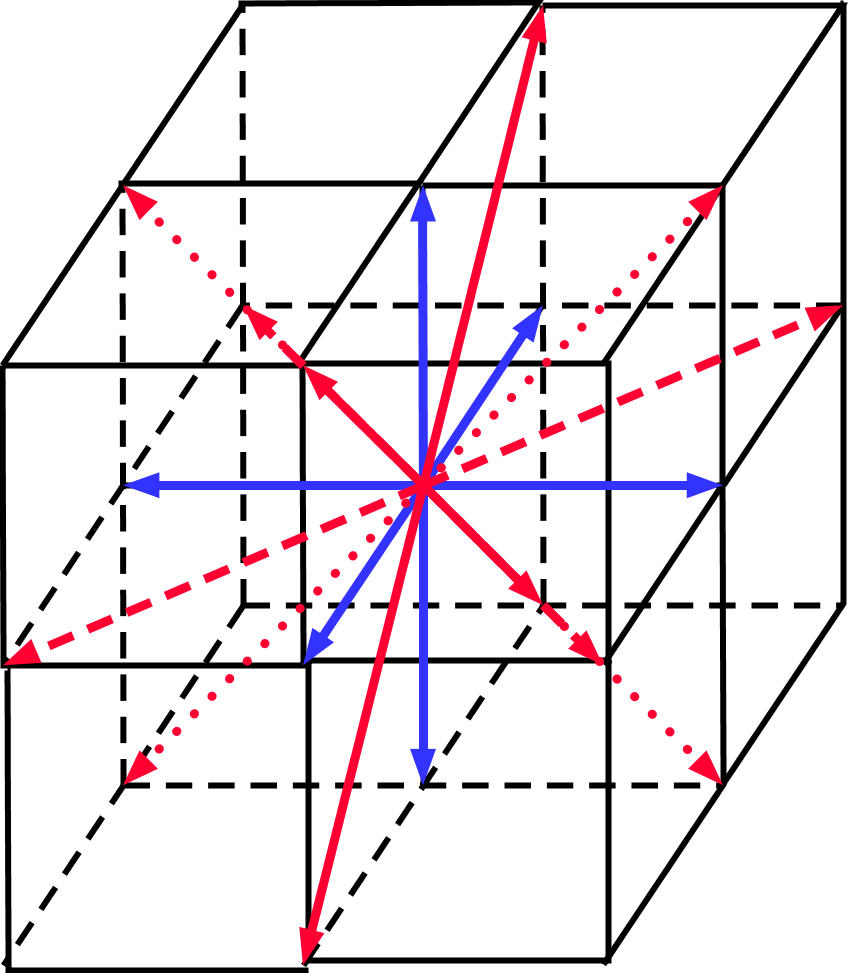
\includegraphics[width=0.6\textwidth]{../obrazky/FCHC}
 \label{fchc}
 \caption{Projection of the lattice vectors into 3D. Red arrows are projections of vectors with $q_4 = 0$,
 blue arrows with $q_4 = \pm 1$.}
\end{figure}

For $q_4 = 0$ we have 12 lattice vectors (red lines on the figure \ref{fchc}), each vector corresponds to the single cell only, so at most one particle propagates along each.
%Hence, at most one particle propagates along each of these vectors.

For both $q_4 = -1$ and $q_4 = 1$ we obtain same six lattice vectors (blue lines on the figure \ref{fchc}). Each vector corresponds to the two cells, hence two particles can propagate along each vector.

In the end, the $3D$ projection of the FCHC lattice leads to the rectangular grid, so the position of the nodes can be denoted by 3 Cartesian integer coordinates.
Each node is connected to 18 neighbors by the lattice vectors of Fig.\ \ref{fchc}, and 24 particles can propagate along them in the single step.

\section{Collision rules for FCHC}

The FCHC lattice was proposed already by Frisch et.\ al.\ in 1986.
However, they did not propose any recipe for collision. It is easy to understand why it is not a simple task.

There are 24 cells in each node, so the node can acquire $2^{24} = 16~777~216$ different states. It was easy to specify the collision rule for FHP in one simple table, but how do you specify rules for millions of states?

In the subsequent section we will show how Henon answered to this challenge in his famous article \cite{henon}.

\bigskip

\subsection{Necessary conditions}

Let us review what are the necessary conditions that collision rules must fulfill:

\begin{enumerate}
\item number of particles is preserved;
\item total momentum is preserved;
\item no other quantity is preserved;
\item exclusion principle -- no two particles occupy one cell in the new state;
\item collision rules are invariant with respect to rotations and reflections of the node;
\item collisions satisfy the semi-detailed balance.
\end{enumerate}

Henon proposed his own conditions on the collisions and showed that all conditions above are automatically fulfilled.

\begin{enumerate}
\item All collisions are isometries of FCHC -- such transformations that preserve set of 24 lattice vectors above. It can be shown that this condition actually defines FHP collision set. For FCHC, this condition guarantees that conditions will be simple and leads us to the simple collision algorithm.

\item The choice of isometry is restricted by the momentum conservation only.
There are 7009 possible values of momentum. But considering that collision rules are invariant under isometries of FCHC, and due to first restriction that collisions are isometries, we can consider 37 momenta only.

\item We want shear viscosity to be as low as possible, so that we can go to higher Reynolds numbers in our simulations. Suppressing the viscosity means is achieved by shortening the mean free path of the particles. In other words, we wish to change as many bits in the collision as possible. We will call such collisions "optimal isometries".

\item The isometry is randomly chosen among optimal isometries.

\end{enumerate}

Having discussed the role of the isometries, let us define them properly.

\section{Isometries of FCHC} 

By $G$ we denote the group of isometries that preserve all 24 lattice vectors (or equivalently all vertexes of FCHC). Any isometry can be represented by $4 \times 4$ matrix
\begin{align}
M = 
\begin{bmatrix}
a_{11} & ... & a_{14} \\
... & & ... \\
a_{41} & ... & a_{44}
\end{bmatrix}.
\end{align}
Although the group G is of order 1152, it can be generated by five elements only,
but it will be more comfortable to employ the generating set consisting of 12 elements to be described in the following section.

\subsection{Generating set}
Isometries $S_{\alpha},~\alpha=1,2,3,4,$ are reflections over(?) plane $x_{\alpha} = 0$.
For example, $S_{1}$ is represented by the matrix
\begin{align}
S_1 = 
\left[\begin{array}{rrrr}
-1 & 0 & 0 & 0 \\
 0 & 1 & 0 & 0 \\
 0 & 0 & 1 & 0 \\
 0 & 0 & 0 & 1
\end{array}\right]
\end{align} 
that flips the sign of the first momentum coordinate $q_{1}$.

\bigskip

Another six isometries $P_{\alpha \beta}$ are reflections over plane $x_{\alpha} = x_{\beta}$.
For example, $P_{12}$ can be represented by matrix
\begin{align}
P_{12} =
\begin{bmatrix}
0 & 1 & 0 & 0 \\
1 & 0 & 0 & 0 \\
0 & 0 & 1 & 0 \\
0 & 0 & 0 & 1
\end{bmatrix}.
\end{align}
that swaps the first and second coordinates of the momentum.

Another isometry $\Sigma_1$ is reflection over plane $x_1 + x_4 = x_2 + x_3$ represented by matrix
\begin{align}
\Sigma_1 = \frac{1}{2}
\left[\begin{array}{rrrr}
1 & 1 & 1 & -1 \\
1 & 1 & -1 & 1 \\
1 & -1 & 1 & 1 \\
-1 & 1 & 1 & 1
\end{array}\right].
\end{align}

The last generating isometry $\Sigma_2$ is reflection over plain $x_1 = x_2 + x_3 + x_4$.
In matrix representation it reads
\begin{align}
\Sigma_2 = \frac{1}{2}
\left[\begin{array}{rrrr}
1 & 1 & 1 & 1 \\
1 & 1 & -1 & -1 \\
1 & -1 & 1 & -1 \\
1 & -1 & -1 & 1
\end{array}\right].
\end{align}

Any isometry of FCHC can be composed from these 12 isometries,
so it can be uniquely expressed by
\begin{align}
M = 
\begin{pmatrix}
I\\
S_4
\end{pmatrix}
\begin{pmatrix}
I\\
S_3
\end{pmatrix}
\begin{pmatrix}
I\\
S_2
\end{pmatrix}
\begin{pmatrix}
I\\
S_1
\end{pmatrix}
\begin{pmatrix}
I\\
P_{34}
\end{pmatrix}
\begin{pmatrix}
I\\
P_{23}\\
P_{24}
\end{pmatrix}
\begin{pmatrix}
I\\
P_{12}\\
P_{13}\\
P_{14}
\end{pmatrix}
\begin{pmatrix}
I\\
\Sigma_1\\
\Sigma_2
\end{pmatrix}
\end{align} 
where the brackets mean ``one of the isometries inside the bracket".


\subsection{Normalized momenta}
Normalized momenta are such momenta that their components fulfill the following two conditions:
\begin{enumerate}
\item $q_1 \geq q_2 \geq q_3 \geq q_4 \geq 0$,  \label{normMom}
\item $q_0 = 0$ or $q_1+g_4 = q_2 + q_3$.
\end{enumerate}


Henon specified collision rules for normalized momenta only. There is 37 normalized momenta (out of 7009 total) so he significantly simplified the job.

If the state has normalized momentum (i.e.\ fulfilling \ref{normMom}), we just look into table and pick any isometry that is offered for that momentum. However, if the state doesn't have normalized momentum,
\begin{enumerate}
\item we normalize it by applying an appropriate isometry on the state. Let us denote this isometry by $\Gamma$. In fact, this isometry is equivalent to the change of the coordinate system.

\item Now that we have state with normalized momenta, search in the table and pick an optimal isometry.

\item We go back to the previous coordinate system by applying isometry $\Gamma^{-1}$.
\end{enumerate}

\subsection{Optimal isometries}

However, in the step 2, we do not want to use all the isometries that conserve the momentum.
Optimally, we would like to change as many bits as possible (that minimizes mean free path of particles, and that leads to desired low viscosity).

Although no further reduction beyond 37 normalized momenta is possible,
some of these momenta share same optimal isometries, that lead to minimal viscosity and preserve momentum.

Based on that,  momenta can be divided into 12 classes, as in the table below.
First column specifies momentum, the second column specifies isometries that can be applied to this momentum. 
Before the simulations starts, we calculate optimal states for each of the $2^{24}$ initial states. Then, the collision step reduces to searching in this huge table and randomly choosing from the available states.

In the early nineties when this algorithm was proposed and tested, the look-up table was considered too big, and several optimizations were proposed and implemented in CRAY-Asssebler \cite{wolf}. Despite that, the achieved update rate was lower then of the Pair-iteraction model, that we are presenting in the next chapter. 
%\begin{tabular}{ |p{1cm}||p{1cm}||p{0.5cm}|p{7cm}|  }
% \hline
% Class& $w_{min}$&\multicolumn{2}{|c|}{Optimal isometries} \\
% \hline
% \hline
% $1$	&	$1/2$	&	$1$	&	$P_{12}$\\
% $2$	&	$1/4$	&	$2$	&	$P_{23}P_{12},\,P_{23}P_{13}$\\
% $3$	&	$1/4$	&	$2$	&	$S_4\Sigma_1,\,S_4\Sigma_2$\\
% $4$	&	$1/2$	&	$1$	&	$S_4$\\
% $5$	&	$1/3$	&	$1$	&	$S_4P_{12}$\\
% $6$	&	$1/4$	&	$4$	&	$S_4\Sigma_1,\,S_4\Sigma_2,\,S_4P_{23}\Sigma_1,S_4P_{23}\Sigma_2$\\
% $7$	&	$1/3$	&	$1$	&	$S_4P_{23}$\\
% $8$	&	$1/4$	&	$4$	&	$P_{23}P_{12},\,P_{23}P_{13},\,S_4P_{23}P_{12},\,S_4P_{23}P_{12}$\\
% $9$	&	$1/3$	&	$3$	&	$S_4S_3,\,S_3P_{34},\,S_4P_{34}$\\
% $10$	&	$1/6$	&	$6$	&	$S_3P_{34}P_{12},\,S_4P_{34}P_{12},\,S_4S_3\Sigma_1,$\\
%		&			&			&	$S_4S_3P_{34}P_{12}\Sigma_1,\,S_4S_3\Sigma_2,\,P_{34}P_{12}\Sigma_2$\\
% $11$	&	$1/6$	&	$6$	&	$S_4S_2P_{23},\,S_4S_3P_{23},\,S_3S_2P_{24},$\\
% 		&			&			&	$S_4S_3P_{24},\,S_3S_2P_{34},\,S_4S_2P_{34}$\\
% $12$	&	$0$	&	$12$	&	$S_3S_1P_{34}P_{12},\,S_4S_1P_{34}P_{12},\,S_3S_2P_{34}P_{12},$\\
% 		&			&			&	$S_4S_2P_{34}P_{12},\,S_2S_1P_{24}P_{13},\,S_4S_1P_{13}P_{13},$\\
% 		&			&			&	$S_3S_2P_{24}P_{13},\,S_4S_3P_{24}P_{13},\,S_2S_1P_{23}P_{14},$\\
% 		&			&			&	$S_3S_1P_{23}P_{14},\,S_4S_2P_{23}P_{14},\,S_4S_3P_{23}P_{14}$\\ 
%\hline 
%\end{tabular}

%\begin{tabular}{ |p{1cm}||p{1cm}||p{0.5cm}|p{9cm}|  }
% \hline
% Class& $w_{min}$&\multicolumn{2}{|c|}{Optimal isometries} \\
% \hline
% \hline
% $1$	&	$1/2$	&	$1$	&	$P_{12}$\\
% $2$	&	$1/4$	&	$2$	&	$P_{23}P_{12},\,P_{23}P_{13}$\\
% $3$	&	$1/4$	&	$2$	&	$S_4\Sigma_1,\,S_4\Sigma_2$\\
% $4$	&	$1/2$	&	$1$	&	$S_4$\\
% $5$	&	$1/3$	&	$1$	&	$S_4P_{12}$\\
% $6$	&	$1/4$	&	$4$	&	$S_4\Sigma_1,\,S_4\Sigma_2,\,S_4P_{23}\Sigma_1,S_4P_{23}\Sigma_2$\\
% $7$	&	$1/3$	&	$1$	&	$S_4P_{23}$\\
% $8$	&	$1/4$	&	$4$	&	$P_{23}P_{12},\,P_{23}P_{13},\,S_4P_{23}P_{12},\,S_4P_{23}P_{12}$\\
% $9$	&	$1/3$	&	$3$	&	$S_4S_3,\,S_3P_{34},\,S_4P_{34}$\\
% $10$	&	$1/6$	&	$6$	&	$S_3P_{34}P_{12},\,S_4P_{34}P_{12},\,S_4S_3\Sigma_1,\,S_4S_3P_{34}P_{12}\Sigma_1,$\\
%		&			&			&	$S_4S_3\Sigma_2,\,P_{34}P_{12}\Sigma_2$\\
% $11$	&	$1/6$	&	$6$	&	$S_4S_2P_{23},\,S_4S_3P_{23},\,S_3S_2P_{24},\,S_4S_3P_{24},$\\
% 		&			&			&	$S_3S_2P_{34},\,S_4S_2P_{34}$\\
% $12$	&	$0$	&	$12$	&	$S_3S_1P_{34}P_{12},\,S_4S_1P_{34}P_{12},\,S_3S_2P_{34}P_{12},\,S_4S_2P_{34}P_{12},$\\
% 		&			&			&	$S_2S_1P_{24}P_{13},\,S_4S_1P_{13}P_{13},\,S_3S_2P_{24}P_{13},\,S_4S_3P_{24}P_{13},$\\
% 		&			&			&	$S_2S_1P_{23}P_{14},\,S_3S_1P_{23}P_{14},\,S_4S_2P_{23}P_{14},\,S_4S_3P_{23}P_{14}$\\ 
%\hline 
%\end{tabular}

\begin{tabular}{ |p{4cm}||p{8.9cm}|  }
 \hline
 Normalized momenta	&	Optimal isometries \\
 \hline
 \hline
 $q_1=q_2>q_3>q_4>0$	&	$P_{12}$\\
 \hline
 $q_1=q_2=q_3>q_4>0$	&	$P_{23}P_{12},\,P_{23}P_{13}$\\
 \hline
 $q_1>q_2>q_3>q_4=0,$	&	$S_4\Sigma_1,\,S_4\Sigma_2$\\
 $q_1=q_2+q_3$				&	\\
 \hline
 $q_1>q_2>q_3>q_4=0,$	&	$S_4$\\
 $q_1 \neq q_2+q_3$		&	\\
 \hline
 $q_1=q_2>q_3>q_4=0$	&	$S_4P_{12}$\\
 \hline
 $q_1>q_2=q_3>q_4=0$	&	$S_4\Sigma_1,\,S_4\Sigma_2,\,S_4P_{23}\Sigma_1,S_4P_{23}\Sigma_2$\\
 \hline
 $q_1>q_2=q_3>q_4=0,$	&	$S_4P_{23}$\\
 $q_q=2q_2$					&	\\
 \hline
 $q_1>q_2=q_3>q_4=0,$	&	$P_{23}P_{12},\,P_{23}P_{13},\,S_4P_{23}P_{12},\,S_4P_{23}P_{12}$\\
 $q_1 \neq 2q_2$				&	\\
 \hline
 $q_1=q_2=q_3>q_4=0$	&	$S_4S_3,\,S_3P_{34},\,S_4P_{34}$\\
 \hline
 $q_1>q_2=q_3=q_4=0$	&	$S_3P_{34}P_{12},\,S_4P_{34}P_{12},\,S_4S_3\Sigma_1,\,S_4S_3P_{34}P_{12}\Sigma_1,$\\
									&	$S_4S_3\Sigma_2,\,P_{34}P_{12}\Sigma_2$\\
 \hline
 $q_1>q_2=q_3=q_4=0$	&	$S_4S_2P_{23},\,S_4S_3P_{23},\,S_3S_2P_{24},\,S_4S_3P_{24},$\\
									&	$S_3S_2P_{34},\,S_4S_2P_{34}$\\
\hline
 $q_1=q_2=q_3=q_4=0$	&	$S_3S_1P_{34}P_{12},\,S_4S_1P_{34}P_{12},\,S_3S_2P_{34}P_{12},\,S_4S_2P_{34}P_{12},$\\
									&	$S_2S_1P_{24}P_{13},\,S_4S_1P_{13}P_{13},\,S_3S_2P_{24}P_{13},\,S_4S_3P_{24}P_{13},$\\
									&	$S_2S_1P_{23}P_{14},\,S_3S_1P_{23}P_{14},\,S_4S_2P_{23}P_{14},\,S_4S_3P_{23}P_{14}$\\ 
\hline 
\end{tabular}

%\begin{figure}
% \centering
% \includegraphics[width=1\textwidth]{./img/Optimal}
%% \label{optimalies}
% \caption{Optimal isometries for 12 momenta classes}
%\end{figure}
\chapter{Pair Interaction LGCA}
Pair-interaction automata (PI) constitute another branch that successfully evolved from HPP model, somewhat in contrast to FHP.
To put it in a nutshell, FHP changed the rectangular grid for hexagonal, and thus obtained better rotational symmetry, increased the degree of freedom of the nodes and added new collision states. 

The pair-interaction model preserves the HPP rectangular lattice, and the degrees of freedom in the node are incremented by the artificial definition of momentum.
%In FHP and HPP, momentum of the particle corresponds to its lattice velocity, or equivalently, to the cell that the particle occupies.
Momenta has no longer same direction as the lattice velocities, but they constitute another degree of freedom of the particle, that might change in the collision, independently of the lattice velocity. 
Although the differentiation in momentum and velocity might seem odd at the first glance, we will show that it leads to the physically correct microdynamics and offers us very efficient algorithm for implementation.

\bigskip
We will explore theory of Pair Interaction automaton in arbitrary dimension later on, but to get good understanding of the pair-interactions, we start with its $2$D version, so we can explain the theory graphically.

\section{User-friendly guide to Pair interactions}

\subsection{Pair-interactions automaton in two dimensions}

Geometry of the lattice is same as for HPP model. It consists of nodes arranged in the rectangular grid:

\begin{figure}[htbp]
 \centering 
 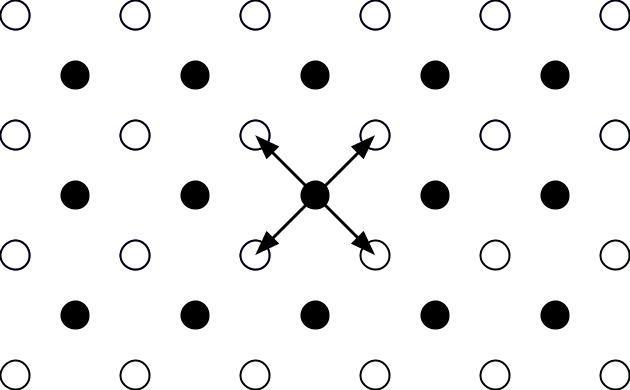
\includegraphics[width=0.9\textwidth]{./img/pi_grid}
 \label{2dgrid}
 \caption{Lattice of 2D Pair Interaction automaton}
\end{figure}

Every node (the cirlce on the picture above) is connected to 4 diagonal neighbors.
Let us consider that in the time-step $t$ only the black nodes are occupied. Then in the next step $t+1$, only the white nodes are occupied. Without loss of generality we can assert that nodes with even Cartesian coordinates, e.g. [0,2], [2,4] are occupied at even time steps, and vice versa. This property of the grid offers very efficient implementation, as  we need only one array for both even and odd time steps.

\bigskip

\textbf{The node:}

Let us look at the node in more detail:
%If we look on the node in more detail, it looks like this:

\begin{figure}[htbp]
 \centering 
 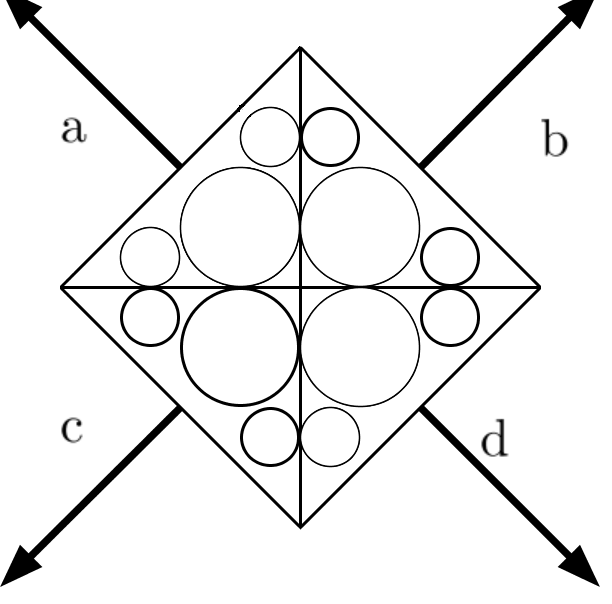
\includegraphics[width=0.3\textwidth]{./img/node_empty}
 \label{empty}
 \caption{A node in detail}
\end{figure}

\newpage
It consists of 4 cells ( \textbf{a,b,c,d} ) that are represented by 3 bits:
% on the picture. Each cell is represented by 3 bits:
one mass bit (a big circle) and two momentum bits (small circles).

The node on the picture above is empty (all bits are set to zero).

Here we have another example of a node:
\begin{figure}[htbp]
 \centering 
 \includegraphics[width=0.5\textwidth]{./img/node_1}
 \label{pre_collision}
 \caption{State of a node before collision}
\end{figure}

In this node, there are particles in the cells a,b,d (mass bit is set to 1 - the big circle is black).

Particle in the cell \textbf{a} is standing (both momentum bits are 0).

Particle in the cell \textbf{b} has momentum in direction [1,1] and particle in the cell \textbf{d} has momentum in direction [0,1].

\subsection{Update rules}
Following rules are true of every lattice-gas cellular automaton.

\begin{enumerate}
\item Lattice is changing in discrete time steps
\item Update rules are \textbf{local}. It means that state of the cell in the next step is determined by the current state of the cell itself and its four neighbors. Hence we can resolve update of the lattice node by node (suitable for parallel computing)
\item If this cellular automaton really simulates fluid dynamics and is physically realistic, update rule needs to conserve \textbf{mass, momentum and angular momentum}.
\end{enumerate}

Update of the lattice is done in two steps, collision and propagation.


\subsection{Collision}
Collision changes configuration inside the single nodes. We require that momentum and mass is preserved in this step.

1) First, the cells are paired in X direction:
\begin{figure}[htbp]
 \centering 
 \includegraphics[width=0.3\textwidth]{../obrazky/x-interaction}
 \label{xinter}
 \caption{Pairs in X-direction}
\end{figure}

Then we swap the bits in the pairs so that total momentum in the pair is preserved. Therefore, node in \ref{pre_collision} changes to

\begin{figure}[H]
 \centering 
 \includegraphics[width=0.5\textwidth]{./img/node_2}
 \label{colision1}
 \caption{State of the node after pair-interaction in X direction}
\end{figure}

2) Then, the cells are paired in Y direction:
\begin{figure}[htbp]
 \centering 
 \includegraphics[width=0.3\textwidth]{../obrazky/y-interaction}
 \label{yinter}
 \caption{Pairs in Y-direction}
\end{figure}

 Then we change the configuration in these pairs preserving mass and momentum in the node. Hence, the node in \ref{colision1} changes into:
 \begin{figure}[htbp]
 \centering 
 \includegraphics[width=0.5\textwidth]{./img/node_3}
 \label{colision2}
 \caption{State of the node after pair-interaction in Y-direction}
\end{figure}
\newpage
Actually, there is only 17 different configurations of the pairs. So instead of computing new configuration during every pair-interaction, we can just look in the table \ref{transitions} below and change the configuration accordingly. We consider this to be the greatest practical advantage of PI comparing to other methods.
\newpage
\begin{figure}[htbp]
 \centering 
 \includegraphics[width=0.7\textwidth]{../obrazky/transitions}
 \label{transitions}
 \caption{All admissible pair-interactions}
\end{figure}

\section{Propagation:}
Particles propagates from a single node to the four neighboring nodes along the lattice vectors, see \ref{2dgrid}.

Particle from the cell \textbf{a} propagates to the node up-right, to the cell \textbf{a} as well.

Analogously, particle from cell \textbf{b} propagates to the node up-left, to the cell \textbf{b}.

Of course, particle carries all its bits (its momentum).



Generalization of this automaton to arbitrary dimension D is very straight-forward. But we need to establish some mathematical formalism, as we haven't learned to draw D-dimensional pictures.

\section{3D Pair-interaction cellular automaton}

\begin{center}
    \begin{tabular}{| l | l | l | l |}
    \hline
    \multicolumn{3}{|c|}{DIFFERENCES BETWEEN \textbf{2}D AND \textbf{N}D PAIR INTERACTION}\\ \hline
     & \textbf{2dim PI CA} & \textbf{Ndim PI CA} \\ \hline
    \textbf{nodes} & $4$ cells arranged into square & $2^D$ cells arranged in hypercube \\ \hline
    \textbf{cells} & 1 mass bit, 2 momentum bits  & 1 mass bit, N momentum bits \\ \hline
    \textbf{neighbors} & node has 4 neighbors & node has $2^D$ neighbors  \\ \hline
    \end{tabular}
\end{center}

In his famous paper, Nasilowski defined and used formalism that:
\begin{enumerate}
\item is more difficult then is necessary in our opinion (and in few cases he redefines it along the way)
\item therefore his arguments are more difficult then necessary
\end{enumerate}


Instead, we will stick to the more modern formalism that we have been using.
We consider it more brief and effective and reader should be already familiar with it.

In previous chapter, reader should get good understanding how 2D Pair-interaction works.
believe that reader has already good idea how 2D Pair-interaction automaton works.

State of the node will be denoted by $\bm{n}(t,\bm{r})$, where $\bm{r}$ is its position on the lattice and $t$ is the current time step. $\bm{n}(t,.)$ represents the whole lattice at time $t$, sometimes we can the time variable and use only $\bm{n}(.)$.

Each node consists of $2^D$ cells:
\begin{equation}
\bm{n} = (n_1, n_2, ... , n_{2^D})
\end{equation}
State of each node is given by $2^D(D+1)$ bits: 
\begin{equation}
\bm{n} = \big\{ n_{i\alpha} \in \big\{0,1\big\},~i = 1..2^D, ~\alpha = 0,1,...D\big\}
\end{equation}
where index $i$ specifies cell of the node, and index $\alpha$ specifies the momentum bit of the cell. Actually, they are the Cartesian coordinates of the cell momenta.



Evolution of the lattice happens in discrete time steps - updates $\mathcal{U}$:

\begin{equation}
\mathcal{U} \bm{n}(t,.) = \bm{n}(t+1,.)
\end{equation} 
Update operator $\mathcal{U}$ can be further divided in two operations, collision $\mathcal{C}$ and propagation $\mathcal{P}$:
\begin{equation}
\mathcal{U} = \mathcal{P} \circ \mathcal{C}
\end{equation} 

\section{Collision}

The purpose of collision is to change the state of the node $\bm{n}$ into new state $\bm{n'}$ such that 2 conditions are fulfilled:

\begin{enumerate}
\item \textbf{Collision operator is one-to-one}:

If $\mathcal{C}: \bm{n} \rightarrow \bm{n'}$,
then $\mathcal{C}: \bm{n'} \rightarrow \bm{n}$.

This reversibility condition allows us to apply Gibbs formalism later on.

\item \textbf{Collision preserves mass and momentum in the nodes}

Mass and momentum are given by
\begin{equation}
m_0 = \sum_i n_{i0}
\end{equation}
\begin{equation}
p_{\alpha} = \sum_i c_{i\alpha} n_{i\alpha},~\alpha=1,2,...D
\end{equation}

Using these definitions, condition of mass and momentum conservation could be expressed by:
\begin{align}\label{mmc}
\begin{split} 
m_o = m'_o &~~ \Leftrightarrow ~~ \sum_i n_{i0} = \sum_i n'_{i0}, \\
p_{\alpha} = p'_{\alpha} &~~ \Leftrightarrow ~~ \sum_i c_{i\alpha} n_{i\alpha} = \sum_i c_{i\alpha} n'_{i\alpha}, ~\alpha=1,2,... D 
\end{split}
\end{align}
\end{enumerate}


The easiest collision rule fulfilling these conditions would be identity
\begin{equation}
\mathcal{I}:\bm{n} \rightarrow \bm{n}
\end{equation}
but this "non-collision" would lead to undesired, non-physical invariants.
On the contrary, we want to change as many bits in the node as possible,
or to say it physically, change directions to as many particles as conservation of momentum allows.
Providing that, the mean free path of particles is reduced to minimum, and we can reach higher Reynold numbers in the simulations.

Such collision algorithm is surprisingly simple and was described in previous section graphically.
Now we state collision rule more formally for arbitrary dimension D.
The algorithm consists of D steps.
In each step ($d=1...D$), we create pairs of cells in $d^{th}$ direction, or equivalently, we create pairs $(n_i,n_j)$, such that $c_{id} = -c_{jd}$ and $c_{i\alpha} = c_{j\alpha}$ for $\alpha \neq d$.
If $n_{id} = n_{jd}$ (it means that in direction $d$, momentum of the pair is zero), we swap the states of the cells $n_i$ and $n_j$ without changing the total momentum of the pairs.
In the end of the collision, the total momentum of the node is conserved, because all the pair-interactions conserved the momentum.

\bigskip

%Parameters $\mu_{\alpha}$ are intensive thermodynamical parameters corresponding to the the extensive dynamical invariants $m_{\alpha}$.

\section{Equilibrium statistics}
We start by revoking the basic result of the microdynamics
\begin{equation} \label{over2}
\bm{n}(t+2,.) = \mathcal{U}^2 \bm{n}(t,.)
\end{equation}

In the odd and even time steps, the different parts of the hlattice are occupied, so it does not make sense to compare them.
That is why we are comparing states of the lattice over the two time steps.

The microdynamical equation \ref{over2} implies conservation of probabilities
\begin{equation} \label{cp}
P(t,\bm{n}(.)) = P(t+2,\mathcal{U}^2\bm{n}(.))
\end{equation}
where $P(t,n(.))$ is the probability of occurrence of lattice in some state $n(.)$ from the statistical ensable of automata.

\subsection{Gibbs distribution}

Let's see if the Gibbs probability distribution fulfill the conservation law \ref{cp}.

First we define the total momentum of the whole lattice $\mathcal{L}$:
\begin{equation} \label{momentum}
m_{\alpha}(.) = \sum_{i,\bm{r}} c_{i\alpha} n_{i\alpha}(\bm{r}),~\alpha=0,1,..D
\end{equation}

Now we can define Gibbs probability for our model:
\begin{equation}
P^E(n(.)) = \frac{W(n(.))}{Z}
\end{equation}
where
\begin{equation}
W(n(.)) = exp(-\sum_{\alpha = 0}^D \mu_{\alpha} m_{\alpha}(.))
\end{equation} 
and $Z$ is the partition function
\begin{equation}
Z = \sum_{n(.))} W(n(.))
\end{equation}

Conservation of local momenta \ref{mmc} implies conservation of the total momentum
\begin{equation}
m_{\alpha}(.) = m'_{\alpha}(.),~\alpha=0,1,..D
\end{equation}
that immediately implies conservation of Gibbs probability
\begin{equation}
P^E(t+2,\mathcal{E}^2n(.)) = P^E(t,n(.)).
\end{equation}

Additivity of the momentum cell by cell over the whole lattice (equation \ref{momentum}) implies that there is no statistical correlation between different cells:
\begin{equation}
P^E(n(.)) = \prod_{i,\bm{r}} P^E(n_i(\bm{r}))
\end{equation} 
Even further, if we consider, that
\begin{equation}
P(n_i(\bm{r})) = \frac{W(n_i(\bm{r}))}{Z}
\end{equation}
where
\begin{equation}
W(n_i(\bm{r}))=exp(-\sum_{\alpha = 0}^D\mu_{\alpha}c_{i\alpha}n_{i\alpha}(\bm{r})) = \prod_{\alpha=0}^Dexp(-\mu_{\alpha}c_{i\alpha}n_{i\alpha}(\bm{r})) = \prod_{\alpha = 0}^D W(n_{i\alpha}(\bm{r}))
\end{equation}
we can see that bits of the cells $n_{i\alpha},~\alpha = 1,2,...D$ are not statistically correlated.

For sure, they are correlated with $n_{i0}$, because $n_{i0} = 0 \Rightarrow n_{i\alpha} = 0~ for~ \forall ~ \alpha = 1,2,...D$.

But for $\alpha=1,2,...D$ we can write:
\begin{equation} \label{form2}
\sigma_{i\alpha} = prob(n_{i\alpha} = 1 | n_{i0} = 1) = \frac{W(n_{i\alpha})}{Z_{i\alpha}}
\end{equation}
where
\begin{equation}
W(n_{i\alpha}) = exp(-\mu_{\alpha}c_{i\alpha}n_{i\alpha})
\end{equation}
and
\begin{equation}
Z_{i\alpha} = \sum_{n_{i\alpha}=0}^1 W(n_{i\alpha}). 
\end{equation}
Hence
%\begin{align}
%\frac{1}{1 + \exp(\mu_{\alpha} c_{i\alpha})} := f(\mu_{\alpha} c_{i\alpha}).
%\end{align}

Little more laborious calculation would lead us to mean occupation numbers
\begin{equation} \label{form1}
\rho_i := <n_{i0}> = \frac{Z_i - 1}{Z_i} = \frac{e^{-\mu_0}\prod_{\alpha = 1}^D(1+e^{-{\mu_{\alpha} c_{i\alpha}}})}{1+e^{-\mu_0}\prod_{\alpha = 1}^D(1+e^{-{\mu_{\alpha} c_{i\alpha}}}) } = f\big(\mu_0 + \sum_{j=1}^d ln f(-\mu_j v_j) \big).
\end{equation}
$\rho_i$ can be interpreted as probability that cell $n_i$ is occupied, but also as the equilibrium mass of the cell.

To define the density, we need to consider what is the volume of the node. Since lattice vectors $c_{i\alpha}$ span interval $[-1,1]^D$, we can define volume V as
\begin{equation}
V = 2^D
\end{equation}
Then the mass density reads
\begin{equation}
\rho = 2^{-D} \sum_i \rho_i
\end{equation}
and the momentum density
\begin{equation}
q_a := 2^{-D} \sum_i c_{i\alpha} <n_{i\alpha}> = 2^{-D} \sum_i c_{i\alpha} \rho_i \sigma_{i\alpha}.
\end{equation}
It is efficient to use only one quantity instead of mass and momentum density, and our formalism invites us to do so. We define the \textbf{hypermomentum} density
\begin{equation} \label{hypermom}
q_{\alpha} := 2^{-D} \sum_i c_{i\alpha} <n_{i\alpha}>
\end{equation}
where $q_0$ is the mass density $\rho$, and $(q_1,q_2,...q_D)$ is the momentum density.

Expanding formulas \ref{form1} and \ref{form2} in Taylor series and inserting to the last equation leads to rather lengthy calculation (Appendix B in [2]), that results in 
\begin{align}
\begin{split}
\rho_i &= \rho + 2 \frac{1-\rho}{2-\rho} \bm{v}.\bm{q} + 2 \, \frac{(1-\rho)(1-2\rho}{(2-\rho)^2 \rho} \, \big[(\bm{v}.\bm{q})^2 - q^2 \big] + O(q^3), \\
\sigma_{ij} &= \frac{1}{2} + \frac{v_j q_j}{(2-\rho)\rho} + O(q^3)
\end{split}
\end{align}
%for $|\bm{q}| \ll 1$.

\section{Hydrodynamic description}
It is based on the assumption that the state of the cellular automaton is near its equilibrium.
In that case, the whole state of the automaton can be specified by a few macroscopic order parameters $q_{\alpha}$.

\bigskip

For example, expectation values $p_{i\alpha}$ are continuous differentiable functions of the parameter q
\begin{equation}
p_{i\alpha} = p_{i\alpha}(q, \nabla q, \nabla^2 q,...)
\end{equation}
and we can expand them in Chapman-Enskog series in terms of $p_{i\alpha}^{eq}$
\begin{equation} \label{expro}
p_{i\alpha} = p_{i\alpha}^{eq} + r_{i\alpha} + \mathcal{O}(\nabla^2)
\end{equation}
with
\begin{align}
r_{i\alpha} = \sum_{\beta j} R_{i\alpha \beta j } \nabla_j q_{\beta}.
\end{align}
We will use this expansion later on.

\bigskip

The resulting equations of this section will be the hydrodynamic equations for the pair-interaction automaton.

They are the set of evolution equations for the order parameters
\begin{equation} \label{evol}
\partial_t q_{\alpha} = \dot{q_{\alpha}}(q,\nabla q, \nabla^2 q,...)
\end{equation}
Due to conservation of the hypermomentum, the right hand side of \ref{evol} must be of the form
\begin{equation}
\dot{q_{\alpha}} = -\sum_k \nabla_k Q_{\alpha k}(q, \nabla q, \nabla^2 q).
\end{equation}

Let us look back to the microdynamical propagation equation
\begin{equation}
n_{i\alpha}(t+1,\bm{r} + \bm{c_i}) = n'_{i\alpha}(t, \bm{r}),
\end{equation}
that directly implies
\begin{equation} \label{micprob}
p_{i\alpha}(t+1, \bm{r} + \bm{c_i}) = p'_{i\alpha}(t, \bm{r}).
\end{equation}
If we expand $p_{i\alpha}(t+1, \bm{r} + \bm{c_i})$ in terms of $p_{i\alpha}(t,\bm{r})$, insert it to \ref{micprob} and apply $2^{-D}\sum_i c_{i\alpha}$ on both sides, we get
\begin{equation} \label{dens}
2^{-D} \sum_i c_{i\alpha} \big[(\partial_t + c_{i\alpha}\nabla_{\alpha}) + \frac{1}{2}(\partial_t + c_{i\alpha}\nabla_{\alpha})^2 + ... \big] p_{i\alpha} = 0
\end{equation}
The right-hand side disappeared because of the conservation of hypermomentum
\begin{equation}
2^{-D} \sum_i c_{i\alpha} p_{i\alpha} = 2^{-D} \sum_i c_{i\alpha} p'_{i\alpha}.
\end{equation}


Analogously to FHP and FCHC model, we can define various temporal and spatial scales (see Table \ref{scalings}) and expand operator of time derivative and space derivative into modes
\begin{equation} \label{exoper}
\begin{split}
\partial_t = \epsilon \partial_t^{(1)} + \epsilon^2 \partial_t^{(2)} + ...\\
\partial_{\alpha} = \epsilon \partial_{\alpha}^{(1)}
\end{split}
\end{equation}

Inserting \ref{expro} and \ref{exoper} into \ref{dens} leads to
\begin{equation}
\begin{split}
0 = 2^{-D} \sum_i c_{i\alpha}(\epsilon\partial_{t}^{(1)} + c_i \nabla_i) p_{i\alpha}^{eq} \\
+ 2^{-D} \sum_i c_{i\alpha}\big[\epsilon^2 \partial_t^{(2)} p_{i\alpha}^{eq} + \frac{1}{2}(\epsilon \partial_t^{(1)} + c_{i\alpha} \nabla_{\alpha})^2 p_{i\alpha}^{eq} \\
+ (\partial_t^{(1)} + c_{i\alpha} \nabla_{\alpha})\sum_{j \beta} R_{\beta j \alpha i}\nabla_{j}q_{\beta} \big] + \mathcal{O}(\nabla^3)
\end{split}
\end{equation}

Each order of $\epsilon$ must vanish separately.

For the terms linear in $\epsilon$ we get
\begin{equation}
2^{-D} \sum_i c_{i\alpha}(\partial_{t}^{(1)} + c_{i\alpha} \nabla_{\alpha}) p_{i\alpha}^{eq} = 0
\end{equation} \label{hydym}
or equivalently in terms of momentum density:
\begin{equation}
\partial_t^{(1)} q_{\alpha} + \sum_k \nabla_k Q_{\alpha k}^0 = 0
\end{equation}
where we used definition of hypermomentum \ref{hypermom},
and defined zero$^{th}$ term of momentum flux tensor $Q_{\alpha k}^0$:
\begin{equation}
Q_{\alpha k}^0 := 2^{-D} \sum_i c_{i\alpha}c_{i k} p_{i\alpha}^{eq}
\end{equation}

We can split equation \ref{hydym} into two -  mass density conservation and momentum conservation:
\begin{equation} \label{hyd1}
\partial_t \rho + \bm{\nabla . g^0}(\rho, \bm{q}) = \mathcal{O}(\nabla^2)
\end{equation}
\begin{equation}
\partial_t q_j + \sum_k \nabla_kQ_{jk}^0(\rho, \bm{q}) = \mathcal{O}(\nabla^2)
\end{equation}
where we used $g_k := Q_{0k}$.

\section{Hydrodynamic limiting cases}
In this section, we will derive hydrodynamic limiting cases of our model, that corresponds to four physical approximations,
namely
\begin{enumerate}
\item compressible Euler equation,
\item acoustic  limit,
\item inviscid incompressible Euler equation,
\item incompressible Euler equation with viscosity.
\end{enumerate}

Starting with equation \ref{hyd1}, blabla dokonci

expand in $\epsilon \ll 1$, that is defined as the Knudsen number (ratio  of mean free path and macroscopic scale).

\bigskip

\textbf{1) Compressible Euler equation}

For physical fluid, the equations read
\begin{align}
\begin{split}
\pd_t \rho + \bm{\nabla . q} = 0, \\
\pd_t q_j + \sum_k \nabla_k \big[ p(\rho) \, \delta_{jk} + \frac{1}{\rho} \, q_j \, q_k = 0
\end{split}
\end{align}

For our model, we need to pick up terms of order
\begin{align}
\begin{split}
\pd_t = O(\epsilon^2), ~ \bm{\nabla} = O(\epsilon^2),~\rho = \frac{1}{2} + O(\epsilon), \bm{q} = O(\epsilon) 
\end{split}
\end{align}
and we get

\begin{align}
\begin{split} \label{O2}
\pd_t \rho + \bm{\nabla.} \big[ \big( \frac{10}{9} - \frac{8}{9} big) \bm{q} \big] &= 0,\\
\pd_t q_j + \sum_k \nabla_k \big[\frac{\rho}{2} \delta_{jk} + \frac{8}{9}q_j\,q_k \big] &= 0
\end{split}
\end{align}

As in case of FHP, the absence of Galilei invariance in our model caused the unphysical dependence of the pressure $p$ on $\rho$.

\bigskip

\textbf{2) Acoustic limit}

Picking up the terms of order
\begin{align}
\pd_t = O(\epsilon),~ \bm{\nabla} = O(\epsilon),~ \rho = \rho_0 + O(\epsilon),~ \bm{q} = O(\epsilon)
\end{align}
leads to linear equations of sound
\begin{align}
\begin{split}
\pd_t \rho + 2\frac{1-\rho_0}{2-\rho_0} \bm{\nabla . q} = 0, \\
\pd_t \bm{q} + \frac{1}{2} \nabla \rho = 0 \,.
\end{split}
\end{align}



\textbf{3) Inviscid incompressible Euler equations}

For the ideal physical fluid (ideal fluid means inviscid and incompressible), the equations read
\begin{align} \label{ideal_phys}
\begin{split}
\bm{\nabla . u} &= 0, \\
(\pd_t + \bm{u.\nabla})\bm{u} + \nabla \Phi &= 0,
\end{split}
\end{align}
with $\Phi = p / \rho_0 = 2 p$ being the kinematic pressure.

For our model, taking terms of order
\begin{align}
\pd_t = O(\epsilon^3), \qquad \bm{\nabla} = O(\epsilon^2), \qquad \rho = \frac{1}{2} + O(\epsilon^2), \qquad \bm{q} = O(\epsilon)
\end{align}
from the expansion (cislo) leads us to
\begin{align}
\begin{split}
\bm{\nabla . q} &= 0, \\ 
(\pd_t + \frac{8}{9}\bm{q.\nabla})\bm{q} + \frac{1}{2} \bm{\nabla} \rho &= 0.
\end{split}
\end{align}

At last, our automaton got the hydrodynamic equations right, as we can easily transform then into \ref{ideal_phys} by setting
\begin{align} \label{transfor}
 \Phi = \frac{4}{9} \rho, \qquad \bm{u} = \frac{8}{9} \bm{q}.
\end{align}  
The $\bm{u}$ is the hydrodynamic velocity and 

Notice that the hydrodynamic velocity $\bm{u}$ is the momentum convection velocity, and can not be interpreted as the mean velocity of particles
\begin{align}
\bm{w} = \frac{\langle \sum_i v_i n_{i0} \rangle}{\langle \sum_i n_{i0} \rangle} = ... = \frac{2(1-\rho)}{(2 - \rho) \rho}\bm{q}.
\end{align}

The reason behind this difference lies in the broken Galilean invariance of our model.
The ratio between the velocities is called the "g-factor" ($g(\rho$), and for our special case, it is equal to
\begin{align}
\bm{w} = \frac{4}{3} \bm{q} = \frac{2}{3} \bm{u}.
\end{align}

It already arised in the FHP and FCHC model (where $g(\rho) \sim 1/2$ for small $\rho$).

\bigskip

\textbf{The Navier-Stokes equations}

For most applications, the inviscid incompressible approximation is too much idealized,
and we would like to find an approximation of Navier-Stokes equations
\begin{align} \label{nst}
\begin{split}
\bm{\nabla . u} = 0, \\
(\pd_t + \bm{u.\nabla}\bm{u} + \nabla \Phi = \nu \nabla^2 \bm{u}
\end{split}
\end{align}
with the friction term on the right hand side, containing the shear viscosity $\nu$.

For our model, the analogous set of equations is obtained by picking up terms
\begin{align}
\pd_t = O(\epsilon^2), \qquad \nabla = O(\epsilon), \qquad, \rho = \frac{1}{2} + O(\epsilon), \qquad \bm{q} = O(\epsilon).
\end{align} 
that leads to
\begin{align}
\begin{split}
\bm{\nabla . q} &= 0,\\ 
(\pd_t + \frac{8}{9} \bm{q . \nabla}) q_j + \frac{1}{2}\nabla_j\rho &= \sum_{klm} T_{jklm}\nabla_l \nabla_m q_k.
\end{split}
\end{align}

Is this set of equations equivalent to Navier-Stokes \ref{nst}?
If we could show that $T_{jklm}$ is isotropic, the equations would be equivalent by the transformation \ref{transfor}.
However, this is not the case, our model do not posses symmetries that forces $T_{jklm}$ to be isotropic.
We need to go to the second approximation to get more information of the tensor $T_{jklm}$.

Lengthy calculation that can be found in \cite{nasilowski} leads to
\begin{align} \label{vistens}
\begin{split}
T_{00km} &= \frac{1}{9} \delta_{kl}, \\
T_{jklm} &= \frac{1}{6} (3 \delta_{jl}\delta_{km} + \delta_{jm} \delta_{lk}(1 + \gamma_{mk}) - 2 \delta_{jklm}).
\end{split}
\end{align}

To see if it is isotropic or not, let us consider simple example of two-dimensional flow in $x_1-direction$
\begin{align}
q_1 = q_1(t,x_2), \qquad q_2 = 0.
\end{align}
Then, the Navier-Stokes equations \ref{nst} reduces to 
\begin{align}
\pd_t q_1 = \nu (\nabla_2)^2 q_1,
\end{align}
where $\nu = T_{1122}$ is the shear viscosity coefficient.

\bigskip

Let us rotate the flow by the angle $\alpha$.
We get
\begin{equation}
\pd_t q'_1 = \nu' (\nabla'_2)^2 q'_1
\end{equation}
where the prime quantities are obtained by transformation 
\begin{equation}
\begin{split}
\bm{x} &= R \, \bm{ x'}, \\
\bm{\nabla} &= R \bm{\nabla}, \\
\bm{q} &= R \bm{q'} \\
T'_{j'k'l'm'} &= \sum_{jklm} T_{jklm} R_{jj'} R_{kk'} R_{ll'} R_{mm'}
\end{split}
\end{equation}
with the orthogonal matrix
\begin{align}
R = \begin{pmatrix}
cos(\alpha) & sin(\alpha) \\
-sin(\alpha) & cos(\alpha)
\end{pmatrix} .
\end{align}
The viscosity transformed into rotated coordinate system reads
\begin{align} \label{rotvis}
\begin{split}
\nu' = T'_{1122} = T_{1122} cos^4(\alpha) + T_{2211} sin^4(\alpha) \\
+ (T_{1111} + T_{2222} - T_{1212} - T_{2121} - T_{1221} - T_{2112})cos^2(\alpha) sin^2(\alpha).
\end{split}
\end{align}
The viscosity tensor in original coordinate system reads
\begin{align}
\begin{split}
T_{1122} = T_{2211} &= \frac{1}{2}, \\
T_{1111} = T_{2222} &= \frac{1}{3}, \\
T_{1212} = T_{2121} &= 0, \\
T_{1221} &= \frac{1}{6}, \\
T_{2112} &= \frac{1}{2}. 
\end{split}
\end{align}

Inserting these components into \ref{rotvis}yields
\begin{align}
\nu' = \frac{1}{2}(cos^4(\alpha) + sin^4(\alpha)),
\end{align}
which clearly shows that the shear viscosity is angle-dependent in contrast with the physical fluid and proves anisotropy of the viscosity tensor \ref{vistens}.


%Now, let us examine momentum flux tensor $Q_{\alpha k}^0$ in a more detail.
%Inserting probabilities $p_{i\alpha}$ from ref., we get:
%\begin{equation}
%blablabla
%\end{equation}
\chapter{From Liouville to Navier-Stokes}
In the previous chapters, we derived hydrodynamic equations for LGCA to find out that they do not match the Eulear and Navier-Stokes equation precisely. This flaw is caused by discrete microdynamics of LGCA, which leads to the Fermi-Dirac distribution.
To treat this flaw, the Lattice-Boltzmann models have emerged.

We may say that Lattice-Boltzmann method stands on the two pillars -- Lattice gas cellular automata are the first pillar, and in this chapter we will establish the second one -- kinetic theory of gasses \cite{tong}.	
%
%Moreover, good understanding of the kinetic theory is a first step to understand the theory of lattice-gas cellular automata.

%
%Lattice-gas cellular automata are the first pillar supporting the Lattice-Boltzmann model.
%In this chapter, we will establish the second pillar -- kinetic theory of gasses \cite{tong}.


%
%On these two pillars -- the Lattice-gas cellular automata and kinetic theory, we will explain the Lattice-Boltzmann model in the subsequent chapter.
%
%As we will show in this chapter, microdynamics of the physical fluid leads to Boltzmann distribution, and starting there, we will derive correct hydrodynamic equations.
%
%The will help us to explain Lattice-Boltzmann model clearly and briefly in the subsequent chapter.
%
%
%
%
%Indeed, were pushed one ladder of abstraction higher to meet the Boltzmann distribution of real fluids.
%
%Model - which have learnt both from the lattice-gas cellular automata and 
% u
%
%In previous chapter we saw that microdynamics of LGCA lead to equilibrium occupation numbers give by Fermi-Dirac distribution.
%
%Although these models do not have discrete microdynamics anymore, they are not CA in its true sense, and they are beyond the scope of this thesis, they should be considered
%to conclude the story of LGCA.

	
\section{Liouville's equation}
Let us start by invoking the Hamiltonian for the $N$ particle system
\begin{align*}
H = \frac{1}{2m} \sum_{i=1}^N p_i^2 + \sum_{i=1}^N V(\bm{r_i}) + \sum_{i<j} U(\bm{r_i} - \bm{r_j})
\end{align*}
where $V$ is the potential of the force $\bm{F}= -\nabla V$, that affects all the particles equally, and $U$ is the potential of the $2$-particle interactions. We require that $U$ is short-ranged, meaning $U(r) \approx 0$ for $r$ of order much larger then is the atomic distance.

As usual in the framework of continuum mechanics, $N$ is a ridiculously large number, something like $N \approx 10^{23}$.

Hence, we represent the state of the system by the probability density function $f(\bm{r},\bm{p},t)$. It specifies the probability that the system is found in the vicinity of point $(\bm{r},\bm{p}) = (\bm{r_1},...,\bm{r_N},\bm{p_1},...,\bm{p_N})$.

As usual, the probability is normalized:
\begin{align*}
\int f(\bm{r},\bm{p},t) \, \dd\bm{r} \, \dd\bm{p} = 1, \quad \dd\bm{p} \dd\bm{r} = \prod_{i=1}^N \dd \bm{r_i} \dd \bm{p_i}.
\end{align*}

Since the microdynamics under consideration is deterministic, the probability density function is locally conserved and we may write its continuum equation
\begin{align} \label{protolui}
\frac{\pd f}{\pd t} + \frac{\pd}{\pd \bm{r}} (\bm{\dot{r}} f) + \frac{\pd}{\pd \bm{p}} (\bm{\dot{p}} f) = 0
\end{align}
If we substitute the Hamilton's equations 
\begin{align*}
\frac{\pd \bm{p}_i}{\pd t} = - \frac{\pd H}{\pd \bm{r}_i},~ \frac{\pd \bm{r}_i}{\pd t} = \frac{\pd H}{\pd \bm{p}_i}
\end{align*}
into the equation \ref{protolui}, we obtain the Liouville's equation
\begin{align*}
\frac{\pd f}{\pd t} + \sum_{i=1}^N \frac{\pd f}{\pd \bm{r_i}} \frac{\pd H}{\pd \bm{p_i}} - \frac{\pd f}{\pd \bm{p_i}}\frac{\pd H}{\pd \bm{r_i}} = 0.
\end{align*}
It is often written using the Poisson brackets
\begin{align} \label{lui}
\frac{\pd f}{\pd t} = \big\{ H, \, f \big\}.
\end{align}

\section{The BBGKY hierarchy}
So far, the transition to probability description did not simplified the problem much -- we are still dealing with the function of $N \approx 10^{23}$ variables.

We need to limit our ambitions and we will focus on the one-particle distribution, defined by
\begin{align} \label{1pd}
f_1(\bm{r_1},\bm{p_1},t) = N \int \prod_{i=2}^N \dd \, \bm{r_i} \dd \, \bm{p_i}
 f(\bm{r},\bm{p},t).
\end{align}
Leaving the particle with index $1$ from the product was arbitrary, because all the particles are identical. This is also the reason why $f_1$ is normalized to $N$:
\begin{align*}
\int f_1(\bm{r_1},\bm{p_1},t) \dd \bm{r_1} \dd \bm{p_1} = N.
\end{align*}
To simplify the notation, we will use $(\bm{p},\bm{r})$ instead $(\bm{p_1},\bm{r_1})$ from now on.

For many purposes, the function $f_1$ captures all we need to know.
For example, it gives us the average density of particles at the spatial point $\bm{r}$
\begin{align} \label{partdens}
n(\bm{r},t) = \int f_1(\bm{r},\bm{p},t) \dd \bm{p},
\end{align}
the average velocity of the particle
\begin{align*}
u(\bm{r},t) = \int \frac{\bm{p}}{m} f_1(\bm{r},\bm{p},t) \dd \bm{p},
\end{align*}
and the energy flux
\begin{align*}
\varepsilon(\bm{r},t) = \int \frac{\bm{p}}{m} E(\bm{p}) f_1(\bm{r},\bm{p},t) \dd \bm{p}.
\end{align*}
To derive the equation governing the evolution of $f_1$, let us see how it varies in time:
\begin{align*}
\frac{\pd f_1}{\pd t} = N \int \prod_{i=2}^N \dd \, \bm{r_i} \dd \, \bm{p_i} \frac{\pd f}{\pd t} = N \int \prod_{i=2}^N \dd \, \bm{r_i} \dd \, \bm{p_i} \big\{ H, \, f \big\}.
\end{align*}
Arranging the terms on the right, we can turn this equation in the form
\begin{align} \label{boltzman}
\frac{\pd f_1}{\pd t} = \big\{ H_1, f_1 \big\} + \Big(\frac{\pd f_1}{\pd t} \Big)_{coll},
\end{align}
where
\begin{align*}
H_1 = \frac{p^2}{2m} + V(\bm{r}).
\end{align*}
We see that the evolution of $f_1$ is governed by the Liouville's equation plus the extra term, the \textit{collision integral}
\begin{align*}
\Big(\frac{\pd f_1}{\pd t} \Big)_{coll} = N(N-1) \int \dd \bm{r_2} \dd \bm{p_2} 
\frac{\pd U(\bm{r} - \bm{r_2})}{\pd \bm{r}} . \frac{\pd}{\pd \bm{p}} \int \prod_{i=3}^N \dd \bm{r_i} \dd\bm{p_i} f(\bm{r},\bm{r_2},...,\bm{p},\bm{p_2},...,t).
\end{align*}
Not surprisingly, it is not determined by the 1-particle distribution, because it does not contain the relation of one particle to all other particles. Some of that information is carried by the \textit{2-particle distribution}
\begin{align*}
f_2(\bm{r},\bm{r_2},\bm{p},\bm{p_2},t) := N(N-1)\int f(\bm{r},\bm{r_2},\bm{r_3},...,\bm{p},\bm{p_2},\bm{p_3},...,t) \prod_{i=3}^N \dd \bm{r_i} \dd \bm{p_i}.
\end{align*}
Using the 2-particle distribution, we can rewritten the collision integral as
\begin{align*}
\Big(\frac{\pd f_1}{\pd t} \Big)_{coll} = \int \dd \bm{r_2} \dd \bm{p_2} \frac{\pd U(\bm{r} - \bm{r_2})}{\pd \bm{r}} . \frac{\pd f_2}{\pd\bm{p}}.
\end{align*}
We see that to follow the evolution of one-particle distribution $f_1$, we also need to know something about the two-particle distribution $f_2$. And again, to know the evolution of the two-particle distribution, we repeat the same procedure as before and find the Liouville-like equation for $f_2$ with additional term containing the three-particle distribution $f_3$.

In general, the evolution of \textit{n-particle distribution} is described by
\begin{align} \label{bgky}
\frac{\pd f_n}{\pd t} = \big\{ H_n, f_n \big\} + \sum_{i=1}^n \int \dd \bm{p_{n+1}} \dd \bm{r_{n+1}} \frac{\pd U(\bm{r_i} - \bm{r_{n+1}}}{\pd \bm{r_i}}).\frac{\pd f_{n+1}}{\pd \bm{p_i}},
\end{align}
where the Hamiltonian 
\begin{align*}
H_n = \sum_{i=1}^n \Big(\frac{\bm{p_i}}{2m} + V(\bm{p_i})\Big) + \sum_{i<j\leq n} U(\bm{r_i} - \bm{r_j})
\end{align*}
includes external forces $V$ and interactions between the $n$ particles.

The set of equations \ref{bgky} is called the \textit{BBGKY hierarchy}.
Instead of the Liouville's equation governing the function of $N \approx 10^{23}$ variables, we have now the set of $10^{23}$ functions.

However, it is more advantageous to work with the hierarchy of equations \ref{bgky}, as it is ready to be approximated. Depending on the particular problem at hands, we decide which terms are important and which terms can be ignored, thus truncating the problem to something manageable.

\section{Boltzmann equation}
Let us derive the most simple and useful of these truncations, the Boltzmann equation
\begin{align*}
\frac{\pd f_1}{\pd t} = \big\{ H_1, f_1 \big\} + \Big(\frac{\pd f_1}{\pd t} \Big)_{coll},
\end{align*}
in the closed form, where collision integral is the expression of $f_1$ alone.
%with the collision integral that is the closed expression for the $f_1$ alone.
%OPRAVIT
%that we already saw. The collision integral depends on the $f_2$. We would like to get rid of this dependence.
%, the closed equation for the $f_1$ alone.
%
%We already saw its general form
%but the collision integral was dependent on $f_2$.

To proceed, let us define two time scales:
the time between particle collisions $\tau$, and the time of the collision itself, $\tau_{coll}$.
In a dilute gas, we have
\begin{align*}
\tau >> \tau_{coll},
\end{align*}
so most of the time, $f_1$ follows the Hamiltonian evolution, with occasional, but abrupt perturbations by the collision. 

What is the rate at which the collision happens?

Let the two particles with momenta $\bm{p_1}$ and $\bm{p_2}$ collide at the point $\bm{r}$, and during the collision, they gain velocities $\bm{p'_1}$ and $\bm{p'_2}$.
We can define the rate of the collision by
\begin{align*}
Rate = \omega(\bm{p_1},\bm{p_2} | \bm{p'_1}, \bm{p'_2}) f_2(\bm{r},\bm{r},\bm{p_1},\bm{p_2}),
\end{align*}
where $\omega$ carries information about the dynamics of the collision, and can be computed from the inter-atomic potential $U$ \cite{tong}.

Next, we focus on the collisions where
\begin{enumerate}
\item one of the particles has specific momentum $\bm{p_1}$ before collision, and gains some unspecified momentum $\bm{p'_1}$ in the collision, or
\item the particle had unspecified momentum $\bm{p'_1}$ before the collision, but gains the specific momentum $\bm{p_1}$ in the collision.
\end{enumerate}
The collision integral governing these collisions contains two terms:
\begin{align*}
\Big( \frac{\pd f_1}{\pd t} \Big)_{coll}= \int \big[ \omega(\bm{p'_1},\bm{p'_2} | \bm{p_1}, \bm{p_2}) f_2(\bm{p'_1},\bm{p'_2}) - \omega(\bm{p_1},\bm{p_2} | \bm{p'_1}, \bm{p'_2}) f_2(\bm{p_1}, \bm{p_2}) \big] \dd \bm{p_2} \dd \bm{p'_1} \dd \bm{p'_2}.
\end{align*}
Considering the symmetries of the process (invariance under time reversal and parity), we have
\begin{align} \label{symm} 
\omega(\bm{p'_1},\bm{p'_2} | \bm{p_1}, \bm{p_2}) = \omega(\bm{p_1},\bm{p_2} | \bm{p'_1}, \bm{p'_2}).
\end{align}
Finally, in order to express the collision integral in terms of $f_1$ instead of $f_2$, we make a non-trivial assumption, that velocities of colliding particles are uncorrelated:
\begin{align} \label{chaos}
f_2(\bm{r},\bm{r},\bm{p_1},\bm{p_2}) = f_1(\bm{r},\bm{p_1})\,f_1(\bm{r},\bm{p_2}).
\end{align}
This assumption is known as a \textit{molecular chaos hypothesis}, and seems quite innocent. However, by supposing that particles are uncorrelated before the collision, but they inevitably become correlated in the collision, we introduce the arrow of time on the scene.

Finally, using \ref{symm} and \ref{chaos}, we can write the collision integral in the form
\begin{align} \label{colint}
\Big( \frac{\pd f_1}{\pd t} \Big)_{coll}= \int \omega(\bm{p'_1},\bm{p'_2} | \bm{p_1}, \bm{p_2}) \big[f_1(\bm{r},\bm{p'_1})f_1(\bm{r},\bm{p'_2}) - f_1(\bm{r},\bm{p_1})f_1(\bm{r},\bm{p_2}) \big] \dd \bm{p_2} \dd \bm{p'_1} \dd \bm{p'_2}
\end{align}
and we can express the \textit{Boltzmann equation}
\begin{align} \label{Boltz}
\frac{\pd f_1}{\pd t}  = \big\{ H_1, f_1 \big\} + \Big(\frac{\pd f_1}{\pd t} \Big)_{coll}
\end{align}
in the closed form.

\section{Equilibrium and detailed balance}
The \textit{equilibrium distribution} is defined such that it does not explicitly depend on the time:
\begin{align*}
\frac{\pd f_1^{eq}}{\pd t} = 0.
\end{align*}
Using the Boltzmann equation, we can express this condition equivalently as
\begin{align*}
\big\{ f_1, H_1 \big\} + \Big( \frac{\pd f_1}{\pd t} \Big)_{coll} = 0.
\end{align*}
If we restrict ourselves to the case with vanishing external force
%This is automatically satisfied if $f$ is the function of $H$, the simple example being the Boltzmann distribution
%\begin{align*}
%f \approx e^{-\beta H}.
%\end{align*}
\begin{align*}
V(\bm{r}) = 0,
\end{align*}
any function of momentum commutes with Hamiltonian and the streaming term $\big\{ f_1, H_1 \big\}$ vanishes.
According to \ref{colint}, to make the collision integral vanish, we need to satisfy the \textit{detailed balance} condition
\begin{align} \label{detailedbalance}
f_1^{eq}(\bm{r},\bm{p_1})f_1^{eq}(\bm{r},\bm{p_2}) = f_1^{eq}(\bm{r},\bm{p'_1})f_1^{eq}(\bm{r},\bm{p'_2}),
\end{align}
or equivalently
\begin{align*}
\log(f_1^{eq}(\bm{r},\bm{p_1})) + \log(f_1^{eq}(\bm{r},\bm{p_2})) = \log(f_1^{eq}(\bm{r},\bm{p'_1})) + \log(f_1^{eq}(\bm{r},\bm{p'_2})).
\end{align*}

According to this equation, the sum of logarithms is conserved in the collision.

As we know, such quantities are either momenta or energy, hence the logarithms are the linear combinations of energy and momenta
\begin{align*}
log(f_1^{eq}(\bm{r},\bm{p})) = \beta(\mu - E(\bm{p}) + \bm{u} \cdot \bm{p}),
\end{align*}
where
\begin{align*}
E(\bm{p}) = \frac{1}{2m} p^2
\end{align*}
and $\beta,\mu$ and $\bm{u}$ are constants.
We need to set the constant $\mu$ such that $f_1$ is normalized, which gives us
\begin{align} \label{mbt}
f_1^{eq} = \frac{N}{V}\big(\frac{\beta}{2\pi m}\big)^{3/2} e^{-\beta m (\bm{v} - \bm{u})^2/2}.
\end{align}
Supposing that $\beta$ is the inverse temperature, this is the Maxwell-Boltzmann distribution.

If we forget about the streaming term $\big\{ H_1, f_1 \big\}$, then the detailed balance condition \ref{detailedbalance} leads to the much larger class of solutions, so called \textit{local equilibrium distributions}
\begin{align} \label{localequil}
f_1^{loc}(\bm{r},\bm{p},t) = n(\bm{r},t) \Big(\frac{\beta(\bm{r},t)}{2\pi m}\Big)^{3/2} \exp \big(-\beta(\bm{r},t)\frac{m}{2}[\bm{v} - \bm{u}(\bm{r},t)]^2 \big)
\end{align}
where $n,\beta$ and $\bm{u}$ are promoted to the functions.
By inserting these distributions into the Boltzmann equation, the collision integral vanishes, but the streaming term stays.

\section{Hydrodynamics}
On the most coarse-grained level, the system in local equilibrium is described by hydrodynamics, with the parameters that do not relax to their equilibrium values immediately, but vary slowly in space and time.
%Just like the termodynamics describes systems in the equilibrium, hydrodynamics describes systems in the local equilibrium, with the parameters that vary slowly in space and time.
%These are quantities that do not relax to their equilibrium values immediately, but change on the much slower scale. 
In this section we will show that these parameters are density $\rho(\bm{r},t)$, temperature $T(\bm{r},t)$ and velocity $\bm{u}(\bm{r},t)$ (thus showing that the functions in \ref{localequil} have their usual meaning).

Let us have an arbitrary function $A(\bm{r},\bm{u})$.
To see how does the function $A$ vary in space, we integrate over the momentum space
\begin{align} \label{averg}
\langle A(\bm{r},t) \rangle = \frac{\int A(\bm{r},\bm{p}) f_1(\bm{r},\bm{p},t) \dd \bm{p}}{\int f_1(\bm{r},\bm{p},t) \dd \bm{p}}.
\end{align}
We are already familiar with the denominator -- it is the particle density function, so we can write
\begin{align*}
\langle A(\bm{r},t) \rangle = \frac{1}{n(\bm{r},t)} \int A(\bm{r},\bm{p}) f_1(\bm{r},\bm{p},t) \dd \bm{p}.
\end{align*} 

Note that the resulting function is a function of space and time, since we computed average only over the momentum variables.

%To see how this averaged function evolve in time
We are interested in the functions $A$ that vanish, when integrated against the collision integral
\begin{align*}
\int A(\bm{r},\bm{p})  \Big( \frac{\pd f_1}{\pd t} \Big)_{coll} \dd \bm{p} = 0.
\end{align*}
Intuitively, this condition is required because we are interested in the quantities that vary slowly, but the collisions are abrupt processes, and the term involving collision integral vary fast.

Substituting the expression for the collision integral \ref{colint} to the last equation, we get
\begin{align*}
\int A(\bm{r},\bm{p_1}) \omega(\bm{p'_1},\bm{p'_2} | \bm{p_1}, \bm{p_2}) \big[f_1(\bm{r},\bm{p'_1})f_1(\bm{r},\bm{p'_2}) - f_1(\bm{r},\bm{p_1})f_1(\bm{r},\bm{p_2}) \big] \dd \bm{p_1} \dd \bm{p_2} \dd \bm{p'_1} \dd \bm{p'_2} = 0.
\end{align*}
Considering the symmetries of $\omega$, this condition is equivalent to
\begin{align*}
\begin{split}
\int \omega(\bm{p'_1},\bm{p'_2} | \bm{p_1}, \bm{p_2}) \big[f_1(\bm{r},\bm{p'_1})f_1(\bm{r},\bm{p'_2}) - f_1(\bm{r},\bm{p_1})f_1(\bm{r},\bm{p_2}) \big] \\ \cross \big[A(\bm{r},\bm{p_1}) + A(\bm{r},\bm{p_2}) - A(\bm{r},\bm{p'_1}) - A(\bm{r},\bm{p'_2}) \big] \dd \bm{p_1} \dd \bm{p_2} \dd \bm{p'_1} \dd \bm{p'_2} = 0
\end{split},
\end{align*}
which holds if
\begin{align*}
A(\bm{r},\bm{p_1}) + A(\bm{r},\bm{p_2}) = A(\bm{r},\bm{p'_1}) + A(\bm{r},\bm{p'_2}).
\end{align*}

So $A$ is a quantity that is conserved during the collision, which is true for the energy, momenta, and trivially, for a constant function, e.g. $A=1$.
These are the \textit{collision invariants} of our interest.

If we plug any collision invariant to the Boltzmann equation \ref{Boltz} and integrate over the momenta variables, the term involving collision integral vanishes
\begin{align*}
\int A(\bm{r},\bm{p}) \Big( \frac{\pd }{\pd t} + \frac{\bm{p}}{m}\cdot \frac{\pd}{\pd \bm{r}} + \bm{F} \cdot \frac{\pd}{\pd \bm{p}} \Big) f_1(\bm{r},\bm{p},t) \dd \bm{p} = 0
\end{align*} 
Because $A$ do not explicitly depend on time, we can put it inside the time derivative, and using integration by part on other terms \textit{per partes} leads to
\begin{align*}
\frac{\pd}{\pd t} \int A f \dd\bm{p} + \frac{\pd}{\pd \bm{r}} \cdot \int \frac{\bm{p}}{m} A f \dd \bm{p} - \int \frac{\bm{p}}{m} \cdot \frac{\pd A}{\pd \bm{r}} f \dd \bm{p} - \int \bm{F} \cdot \frac{\pd A}{\pd \bm{p}}f \dd \bm{p} = 0
\end{align*}
Finally, applying the expression for the average \ref{averg} on this equation, we can write
\begin{align} \label{master}
\frac{\pd}{\pd t} \langle n A \rangle + \frac{\pd}{\pd \bm{r}} \cdot \langle n \bm{u} A \rangle - n \langle\bm{u} \cdot \frac{\pd A}{\pd \bm{r}} \rangle - n \langle \bm{F} \cdot \frac{\pd A}{\pd \bm{u}} \rangle = 0,
\end{align}
which is our master equation governing the evolution of the collisional invariant.
In between, we have introduced notation for the velocity
\begin{align*}
\bm{v} = \frac{\bm{p}}{m},
\end{align*}
and now we introduce the average velocity
\begin{align*}
\bm{u} = \langle \bm{v} \rangle.
\end{align*}


Substituting the constant $A=1$ into the master equation yields
\begin{align*}
\frac{\pd n}{\pd t} + \frac{\pd}{\pd \bm{r}} \cdot (n \bm{u}). 
\end{align*}
Multiplying by particle mass $m$, this is the continuity equation.

Substituting the next collisional invariant, the momentum $A=m\bm{v}$, yields
\begin{align} \label{conmom}
\frac{\pd}{\pd t} (mn u_i)  + \frac{\pd}{\pd r_j}\langle mn v_i v_j \rangle - \langle n F_i \rangle = 0
\end{align}
If we expand the middle term like
\begin{align*}
\langle v_i v_j \rangle = \langle (u_j - v_j) (u_i - v_i) \rangle + v_i\, v_j
\end{align*}
and if we define the quantity
\begin{align*}
P_{ij} = P_{ji} = \rho \langle (u_j - v_j) (u_i - v_i) \rangle
\end{align*}
known as the pressure tensor,
we can rewrite the equation \ref{conmom} as
\begin{align} \label{mmcl}
\rho \Big(\frac{\pd}{\pd t} + u_j \frac{\pd}{\pd x_j} \Big) u_i = \frac{\rho}{m} F_i - \frac{\pd}{\pd x_j}P_{ij}.
\end{align}
This is the familiar form of the momentum conservation law. We can interpret it according to the Newton's law -- the left-hand side is the acceleration of the fluid element, and the right-hand side involves the external force $\bm{F}$ and the internal pressure of the fluid
%The collision integral reflects the rate of the collisions.

If we evaluate the pressure tensor on the equilibrium distribution, we find out that it is proportional to the temperature
\begin{align*}
P_{ij} = n k_B T \delta_{ij},
\end{align*} 
which is the ideal gas law.

\bigskip

The last collisional invariant is the kinetic energy of particles.
Instead of absolute kinetic energy, we shall use the relative kinetic energy
\begin{align*}
A  = \frac{1}{2} m (\bm{u} - \bm{v})^2,
\end{align*}
so when we substitute it into our master equation \ref{master}, we get the compact form
\begin{align} \label{cone}
\frac{1}{2} \frac{\pd}{\pd t} \langle \rho(\bm{v} - \bm{u}) \rangle + \frac{1}{2} \frac{\pd}{\pd r_i} \langle \rho v_i (\bm{v} - \bm{u}) \rangle - \rho \langle v_i \frac{\pd u_j}{\pd r_i}(\bm{v} - \bm{u})^2 \rangle = 0.
\end{align}
Using the idea of equipartition, we can define the temperature for the non-equilibrium system
\begin{align*}
\frac{3}{2}k_B T(\bm{r},t) = \frac{1}{2} m \langle (\bm{v} - \bm{u}(\bm{r},t))^2. \rangle
\end{align*}

Let us define another quantity, the \textit{heat flux}
\begin{align*}
\frac{1}{2} m \rho \langle (v_i - u_i)(\bm{v} - \bm{u})^2 \rangle.
\end{align*}
Using the definition of heat flux and pressure tensor, we rewrite the equation \ref{cone} as
\begin{align*}
\frac{1}{2}m \rho \langle v_i (\bm{v} - \bm{u})^2 \rangle = q_i + \frac{3}{2}\rho u_ik_B T,
\end{align*}
Since the pressure tensor is symmetric, we can replace $\pd u_j / \pd r_i$ with the symmetric \textit{rate of strain}
\begin{align*}
U_{ij} = \frac{1}{2}\big( \frac{\pd u_j}{\pd r_i} + \frac{\pd u_i}{\pd r_j} \big).
\end{align*}
Further, using the continuity equation, we obtain the conservation of energy in its usual form
\begin{align*}
\rho \big( \frac{\pd}{\pd t} + u_i \frac{\pd}{\pd r_i} \big) k_B T + \frac{2}{3} \frac{\pd q_i}{\pd r_i} + \frac{2m}{3} U_{ij} P_{ij} = 0.
\end{align*}

Finally, we have the three equations, describing the time evolution of the particle density $n$, momentum $\bm{u}$ and the temperature $T$.
Although they hold for any distribution $f_1$, they do not constitute the closed set of equations -- equation for $n$ depends on $\bm{u}$, equation for momentum depends on the pressure tensor $P_{ij}$ and the equation for temperature depends on the heat flux $q$. To determine any of these, we need to compute the distribution $f_1$ from the Boltzmann equation, which is not easy.

Since we are looking for the solution that varies slowly, the first approximation would be the  local equilibrium distribution \ref{localequil}, for which collision integral vanishes.
%
%Since local equilibrium distribution is not solution of the Boltzmann equation, because streaming term is non-zero, we will see later on what we are missing.
Using this distribution, we can compute that
\begin{align*}
P_{ij} = k_b n(\bm{r},t) T(\bm{r},t) \delta_{ij} = P(\bm{r},t) \delta_{ij}
\end{align*} and
\begin{align*}
q = 0.
\end{align*}
Inserting these terms into the conservation laws, the continuity equation stays unchanged, we just rewrite it using $\rho = m\,n$:
\begin{align} \label{cunt}
\big(\frac{\pd}{\pd t} + u_j \frac{\pd}{\pd r_j} \big) \rho + \rho \frac{\pd u_i}{\pd r_i}.
\end{align}
However, the momentum conservation \ref{mmcl} turns into the Euler equation
\begin{align} \label{ell}
\big(\frac{\pd}{\pd t} + u_j \frac{\pd}{\pd r_j} \big) u_i  + \frac{1}{\rho}  \frac{\pd P}{\pd x_i} = \frac{F_i}{m}.
\end{align}
However, we are still missing dissipation in these equations. To show it, we can combine equations \ref{cunt} and \ref{ell} to obtain
\begin{align*}
\big( \frac{\pd}{\pd t} + u_j \frac{\pd}{\pd r_j} \big) (\rho T ^{-2/3}) = 0
\end{align*}
This equation implies that $\rho T^{-2/3}$ is constant along the streamlines, which means that the motion of the fluid is adiabatic -- not increasing entropy. Hence we have no mechanism for the fluid to return to the equilibrium yet.

It is easy to see what we are missing. We chose local equilibrium as an approximation for the distribution $f_1$, so that the collision integral vanishes, but it does not solve the streaming term. However, if we stick to the long wave-length variations in the velocity, we need to add only little correction term
\begin{align} \label{cord}
f_1 = f_1^{(0)} + \delta f_1.
\end{align}
The correction $\delta f_1$ contributes to the collision integral
\begin{align*}
\Big( \frac{\pd f_1}{\pd t} \Big)_{coll}= \int \omega(\bm{p'_1},\bm{p'_2} | \bm{p_1}, \bm{p_2}) \big[ f_1(\bm{p'_1})f_1(\bm{p'_2}) - f_1(\bm{p_1})f_1(\bm{p_2}) \big] \dd \bm{p_2} \dd \bm{p'_1} \dd \bm{p'_2}
\end{align*}
where we neglected the quadratic terms $O(\delta f_1^2)$ and used the fact that $f_1^{(0)}$ vanish in the collision integral.

To proceed further, the proper way would be to use \textit{Chapman-Enskog expansion} of $\delta f_1$ to treat the collision operator properly, but there is an easier way to progress, the so called $BGK$ \footnote{Bhatnagar-Gross-Krook} approximation. We simply set the collision integral to be
\begin{align} \label{bgk}
\Big( \frac{\pd f_1}{\pd t} \Big)_{coll} = - \frac{\delta f_1}{\tau},
\end{align}
where $\tau$ is the relaxation time, and we take it to be a constant (although in general, it might be function of momentum).
With this replacement, the Boltzmann equation changes to
\begin{align*}
\frac{\pd (f_1^{(0)} + \delta f_1)}{\pd t} - \big\{ H_1, f_1^{(0)} + \delta f_1 \big\} = -\frac{\delta f_1}{\tau}
\end{align*}

\section{Where is the viscosity?}
Let us consider the flow of the fluid with the velocity gradient $\pd u_x / \pd z \neq 0$.
According to the Newton's law, the shear viscosity is associated with the flux of $x$-momentum to the $z$-direction:
\begin{align} \label{newt}
\Pi_{xz} = -\eta \frac{\pd u_x}{\pd r_z},
\end{align}
which is the off-diagonal component of the pressure tensor
\begin{align*}
P_{xz} = \rho \langle (v_x - u_x) (v_z - u_z) \rangle.
\end{align*}

As we already know, the local equilibrium distribution gives us the diagonal pressure tensor, but if we use the corrected distribution, we have
\begin{align}
P_{ij} = P \delta_{ij} + \Pi_{ij},
\end{align}
with the additional term $\Pi_{ij}$, which is a non-diagonal \textit{stress tensor}
\begin{align*}
\Pi_{ij} = \frac{m \tau \rho}{k_B T} U_{kl} = \Big[ \langle v_i v_j v_k v_l \rangle_0 - \frac{1}{3} \delta_{kl} \langle v_i v_j v^2 \rangle_0 \Big].
\end{align*}
In fact, the $\Pi_{ij}$ is traceless, because
\begin{align*}
\langle v^2 v_k v_l \rangle_0 = \delta_{kl} \langle v_i v_j v^2 \rangle_0. 
\end{align*}
and it depends linearly on the $U_{kl}$.
These two properties determine the form of the tensor
\begin{align} \label{stresst}
\Pi_{ij} = -2 \mu \big( U_{ij} - \frac{1}{3} \delta_{ij} \nabla . \bm{u} \big).
\end{align}
For $\pd u_x / \pd z \neq 0$, we can evaluate
\begin{align*}
\Pi_{xz} = \frac{2m\tau \rho}{15k_B T} U_{xx} \langle v^4 \rangle_0.
\end{align*}
Comparing it to the Newton's law \ref{newt}, we get an expression for the shear viscosity
\begin{align} \label{shearv}
\eta = n k_B T \tau.
\end{align}

Note that this expression is just an estimation, as it relies on the relaxation time approximation $\tau$.

\section{Navier-Stokes equations}

The corrected distribution \ref{cord} does not change the density equation
\begin{align*}
\frac{\pd \rho}{\pd t} + \nabla . (\rho \bm{u}) = 0,
\end{align*}
but due to the non-diagonal stress tensor \ref{stresst}, the momentum equation transforms to the Navier-Stokes equation
\begin{align}
\Big(\frac{\pd}{\pd t} + \bm{u} \cdot \nabla \Big) \bm{u} = \frac{\bm{F}}{m} - \frac{1}{\rho} \nabla P + \frac{\eta}{\rho} \nabla^2 \bm{u} + \frac{\eta}{3 \rho}\nabla(\nabla \cdot \bm{u})
\end{align}
%Since $\nabla \kappa \approx 0$ and $U_{ij} \Pi_{ij} \approx 0$ are small at the order we are working at, we can drop them and the equation reduces to
%\begin{align*}
%aa
%\end{align*}
Although our derivation relied on the dilute gas approximation, the Navier-Stokes equation are more general then that and can be considered to be the most general expression for the momentum transport \cite{tong}.

%This force K will be neglected in the subsequent text, because external force is not supposed to influence dynamics of collisions.
%The right hand side of Boltzmann equation, the $Q(f,f)$, is the collision integral.
%It is quite complicated expression
%and it is the major difficulty in dealing with Boltzmann equation.
%But we do not need it that precisely, as two-particle collisions do not significantly influence experimentally measured quantities.
%Therefore, it is often approximated.
%Before we show the standard way to approximate it (so called BGK approximation), we need to present the properties of $Q(f,f)$ that need to be preserved.

%Interestingly, function 
%\begin{align} \label{nulling}
%\phi = \exp (a + \bm{b}. \bm{v} + c \, v^2)
%\end{align}
%is the solution of
%\begin{align}
%Q(f,f) = 0,
%\end{align}
%if $c$ is negative. Notice, that famous Maxwell function (or Maxwell distribution, or simply Maxwellian) is the spacial kind of such function \ref{nulling} 
%\begin{equation} \label{Maxwell}
%f^M(\bm{x,v,}t) = n(\frac{m}{2 \pi k_B T})^{3/2} e^{-\frac{m}{2k_B T}(\bm{v-u})^2}.
%\end{equation}
%
%Now we are ready to state what is BGK approximation of collision integral $Q(f,f)$.
%\section{BGK approximation}
%Instead of $Q(f,f)$, that is so complicated we do not even state it, we will use simpler operator 
%\begin{align}
%J(f) = w[f^M(\bm{x,v}) - f(\bm{x,v}]
%p\end{align}
%
%We can easily see that this approximation have two properties:
%\begin{enumerate}
%\item It expresses the tendency of $f$ towards Maxwellian distribution \ref{Maxwell} (because the time derivative of $f$ has sign towards $f^M$).
%\item It conserves the collision invariants \ref{invariants}
%\begin{align}
%\int \psi_k J(f) d^3 x d^3 v = 0
%\end{align}
%\end{enumerate}
%
%
%\section{Chapman-Enskog series}
%We are already familiar with this kind of expansion, now we will show it in the general context.
%In some respect this expansion is quite peculiar and deserves few comments before we suck the life out of it.
%
%\bigskip
%
%The distribution function f, that is explicitly time-dependent, will be expanded in the series of $f^{(n)}$, that have only implicit time-dependence. However, gas relaxes very fast, in time of order $10^{-11}$ seconds, towards time-independent distributions, hence this expansion is generally valid.
%
%
%The expansion parameter $\epsilon$ depended on the peculiarities of our model in previous chapters. 
%In this section, we will take $\epsilon$ equal to Knudsen number
%\begin{align}
%K_n = \frac{\lambda}{L},
%\end{align}
%that is ratio of $\lambda$, the mean free path of particle (the mean distance between two successive collisions) and spatial characteristic scale $L$ (for example, size of the obstacle in the flow, diameter of the flow etc.).
%
%\bigskip
%
%And the most interesting point comes last - the Chapman-Enskog series diverges.
%
%We are interested only in first two orders of the expansion, but higher order-approximation that lead to Burnett equations are problematic and were never applied systematically (for further details see Cercignani 1988 and 1990).
%
%
%\section{Conservation laws}
%What happens if we multiply Boltzmann equation with the collision invariants \ref{invariants} and integrate it?
%
%Since the collision integral in the right-hand side gets killed-off (by definition of invariants), 
%the equation reads
%\begin{equation}
%\int \psi_k(\partial_t + v_{\alpha}\partial_{\alpha}) f(\bm{x},\bm{v},t) d^3v = 0.
%\end{equation}
%Substituting $\psi_0 = 1$, $(\psi_1,\psi_2,\psi_3) = \bm{v}$ and $\psi_4 = v^2$, we get the general form of conservation laws:
%
%\begin{align}
%\begin{split}
%\partial_t\rho + \partial_{\alpha}(\rho u_{\alpha}) &= 0 \\
%\rho \partial_t u_{\alpha} + \rho u_{\beta}\partial_{\beta}u_{\alpha} &= - \partial_{\alpha}\hat{P}_{\alpha\beta} \\
%\rho \partial_t \Theta + \rho u_{\beta}\partial_{\beta}\Theta &= -\frac{2}{3} \partial_{\alpha}q_{\alpha} - \frac{2}{3} \hat{P}_{\alpha\beta} \Lambda_{\alpha\beta}
%\end{split}
%\end{align}
%where
%\begin{align}
%\begin{split}
%n(\bm{x}, t) &= \int f(\bm{x},\bm{v},t) \, d^3 v  \\
%p(\bm{x},t) &= m \, n(\bm{x},t) \\
%\rho u_{\alpha}(\bm{x},t) &= m \int v_{\alpha} f(\bm{x},\bm{v},t) \, d^3 v \\
%\Theta(\bm{x},t) &= k_B \, T(\bm{x},t) = \frac{m}{3n} \int (v_{\alpha} - u_{\alpha})(v_{\alpha} - u_{\alpha}) \, f(\bm{x},\bm{v},t) \, d^3 v \\
%\Lambda_{\alpha\beta} &= \frac{m}{2} (\pd_{\beta}u_{\alpha} + \pd_{\alpha} u_{\beta}) \\
%\hat{P}_{\alpha\beta} &= m \int (v_{\alpha} - u_{\alpha})(v_{\beta} - u_{\beta}) \, f(\bm{x}, \bm{v}, t) \, d^3v \\
%q_{\alpha}(\bm{x},t) &= \frac{m^2}{2} \int (v_{\alpha} - u_{\alpha})(v_{\beta} - u_{\beta}) (v_{\beta} - u_{\beta}) \, f(\bm{x}, \bm{v}, t) \, d^3v
%\end{split}
%\end{align}
%
%\section{Euler equation}
%
%$f^M$ into conservation laws:
%$\partial_t \rho + \partial_{\alpha}(\rho u_{\alpha}) = 0$ ... continuity equation\\
%$\rho \partial_t u_{\alpha} + \rho u_{\beta}\partial_{\beta}u_{\alpha} = - \partial_{\alpha}P$ ... Euler equation,\\
%where $P = n\Theta = n k_B T$\\
%$\rho \partial_t \Theta + \rho u_{\beta}\partial_{\beta}\Theta = -\frac{1}{c_V} \Theta \partial_{\alpha} u_{\alpha}$\\
%
%Chapman-Enskog:\\
%$f = f^0 + \epsilon f^1 + \epsilon^2 f^2 + ... = $
%
%It is special in every sense of word, we will introduce some of its useful properties:
%\chapter{From Boltzmann to Navier-Stokes}

Because microdynamics of LGCA lead to equilibrium occupation numbers given by Fermi-Dirac distribution, there is no way to improve them substantionally u

In previous chapter we saw that microdynamics of LGCA lead to equilibrium occupation numbers give by Fermi-Dirac distribution.
Treatment of the symptoms resulting from this flaw is imperfect.

In this chapter we will show what statistical properties would be desirable for better computational model.
We will show that microdynamics of physical fluid lead to Boltzmann distribution, and starting there, we will derive Navier-Stokes equations in its most general form.
 
Indeed, the new generation of LGCA, the Lattice-Boltzmann models, were pushed one ladder of abstraction higher to meet the Boltzmann distribution of real fluids.
But since these models do not have discrete microdynamics anymore, they are not CA in its true sense, and they are beyond the scope of this thesis.
However, we would like to show some light at the tunnel and motivate the method, that is an efficient competitor to other CFD methods.

\bigskip
The name of the chapter is shamelessly stollen from \cite{wolf}. In the original piece, it precedes chapter on Lattice-Boltzman model and is full of technicalities (we have seen Chapman - Enskog expansion already), we rather follow approach of \cite{astro}, that offers better physical insight.

In Wolf-Gladrow, the derivation of Navier-Stokes is performed by the means of Chapman-Enskog expansion.
We chose approach from \cite{astro}, as it offers us better physical insight with less technicalities then \cite{wolf}, where the derivation of Navier-Stokes is performed by the means of Chapman-Enskog expansion.

\section{Boltzmann equation}

Let us consider an enslable of identical particles. Quantum effects, such as internal degrees of freedom in particles will be neglected. The state of the ensamble will be given by distribution function $f(\bm{x}, \bm{u}, t)$, that is defined by
\begin{equation} \label{hust}
dN = f(\bm{x}, \bm{u}, t) d\bm{x} \, d\bm{u}
\end{equation} 
where $dN$ is the number of particles in the infinitesimal phase element $[x, x+ dx] \cross [u, u +du]$.
It must be emphasized that statistical description is appropriate only if $dN$ is sufficiently large number.

Let us suppose that external force field $\bm{F} = (F_1, F_2, F_3)$ is affecting the system such that it is same for all particles in volume element $[x, x+ dx]$. This assumption is reasonable, since the particles are infinitesimally close.

Then, at any time $t$ the velocity of the particles in the element $[x, x + dx]$ will change from (let's say) $\bm{u'}$ to $\bm{u'} + \bm{F}dt$.

\begin{align*}
\pd_t f + \bm{v}.\nabla f + \frac{\bm{K}}{m}\pd_{\bm{v}} f = Q(f,f)
\end{align*}

Thus, if we neglect the collisions between particles, we can say, that number of particles 
$f(\bm{x}, \bm{u}, t)$ is equal to $f(\bm{x + u}dt, \bm{u + F}dt, t + dt)$, or 
\begin{align*}
f(\bm{x}, \bm{u}, t) - f(\bm{x + u}dt, \bm{u + F}dt, t + dt) = 0.
\end{align*}
If we consider the collisions between particles, we need to write
\begin{align*}
f(\bm{x}, \bm{u}, t) - f(\bm{x + u}dt, \bm{u + F}dt, t + dt) = [\Delta f]_{coll},
\end{align*}
where right hand side stands for change of $f$ in a time interval $dt$ due to collisions.

Since the left hand side is the difference of function values in infinitesimal time difference $dt$, we can write it in the differential form
\begin{align} \label{BoltzmannE}
\frac{\pd f}{\pd t} + u_i \frac{\pd f}{\pd x_i} + F_i \frac{\pd f}{\pd u_i} = \big[\frac{\pd f}{\pd t} \big]_{coll}.
\end{align}

This is the famous Boltzmann equation and we derived it in very intuitive way. We need to mention three subtle assumptions that Boltzmann used to derive it.
\begin{enumerate}
\item Only one-particle collisions are considered (so it would apply only to diluted gas).
\item \textit{Molecular chaos hypothesis} - velocities of colliding particles are uncorrelated.
\item External forces do not influence the dynamics of collisions.
\end{enumerate}

\section{Macroscopic quantities}
To obtain the volume density of particles $n(\bm{x},t)$, we integrate the probability density function $f(\bm{x},\bm{u},t)$ over velocity coordinates:
\begin{align*}
n(\bm{x},t) = \int f(\bm{x,u},t) \dd \bm{x} \dd \bm{u}.
\end{align*}

Then the mass density is
\begin{align} \label{densb}
\rho(\bm{x},t) = \int m \, f(\bm{x,u},t) \dd \bm{u},
\end{align}
and the mean velocity of the flow
\begin{align} \label{meanv}
\bm{v}(\bm{x},t) = \int \bm{u} \, f(\bm{x,u},t) \dd \bm{u}.
\end{align}

For the low densities we can neglect many-particle collisions and  consider only two-particle collisions that are elastic (preserving energy and momentum of the colliding pair).
Then, the density function $f$ is the famous Maxwell function
\begin{equation} \label{Maxwell}
f^M(\bm{x,v,}t) = n(\frac{m}{2 \pi k_B T})^{3/2} e^{-\frac{m}{2k_B T}(\bm{v-u})^2}.
\end{equation}

\section{Hydrodynamic equations}
The right hand side of \ref{boltzmanE} is often referred to as collision integral and is a lengthy expression that we do not to state explicitly, but its general properties can be analyzed nevertheless.

Since the collisions among the particles preserve the number of particles in the system, we have
\begin{align} \label{consm}
\int \Big[\frac{\pd f}{\pd t} \Big]_{coll} \dd \bm{u} = 0.
\end{align}
The total momentum is also preserved by the collisions, so
\begin{align} \label{consmm}
\int \bm{u} \Big[\frac{\pd f}{\pd t} \Big]_{coll} \dd \bm{u} = 0,
\end{align}
and finally, the total energy is conserved by the collisions, hence
\begin{align} \label{conse}
\int u^2 \Big[\frac{\pd f}{\pd t} \Big]_{coll} \dd \bm{u} = 0.
\end{align}

And because the total energy of the system is finite, it must be true that
\begin{align} \label{lime}
\lim_{u \rightarrow \infty} u^2 f = 0.
\end{align}

Using this limit and performing integration by parts on equations \ref{consm} -- \ref{conse} leads to
\begin{align} \label{due}
\int \frac{\pd f}{\pd u_i} \dd \bm{u} = 0,
\end{align}
\begin{align} \label{due2}
\int u_i \frac{\pd f}{\pd u_i} \dd \bm{u} = -\delta_{ij} \frac{\rho}{m},
\end{align}
\begin{align}
\frac{1}{2} \int u^2 \frac{\pd f}{\pd u_i} \dd \bm{u} = - v_i \frac{\rho}{m}.
\end{align}


Now that we are equipped with equations above, let us multiply the Boltzmann equation by $m$ and integrate over the whole domain. We obtain
\begin{align}
m \int \frac{\pd f}{\pd t} \dd \bm{u} + m \int u_i \frac{\pd f}{\pd x_i} \dd \bm{u} + m F_i \int \frac{\pd f}{\pd u_i} \dd \bm{u} = 0,
\end{align}
where right-hand side is zero due to equation \ref{consmm}.

We can delete the third term due to \ref{due}, and since $\bm{u}$ and $\bm{x}$ are considered to be independent variables in the phase space, we can swap the integration by $u_i$ and derivation by $x_i$ and $t$. Hence we get
\begin{align}
\frac{\pd }{\pd t} \int m \, f \dd \bm{u} + \frac{\pd}{\pd x_i} \int u_i \, m \, f \, \dd \bm{u} = 0,
\end{align}
and applying definition of density \ref{denb} and mean velocity \ref{meanv}
we can write in the form
\begin{align}
\frac{\pd \rho}{\pd t} + \frac{\pd}{\pd x_i}(\rho v_i) = 0.
\end{align}
This is the common form of continuity equation, or law of mass conservation.

If we multiply the Boltzmann equation by the mass $m$ and integrate over the whole domain again, we get
\begin{align} \label{primeul}
\frac{\pd}{\pd t} (\rho \, v_i) + \frac{\pd }{\pd x_j} \int m \, u_i \, u_j \, f \, \dd \bm{u} - \rho \, F_i = 0,
\end{align}
where we used equality \ref{due2}.

We can break down the second term into
\begin{align} 
\int m \, u_i \, u_j \, f \, \dd \bm{u} = \int m \, v_i \, v_j \, f \dd \bm{u} + \int (v_i - u_i) (v_j - u_j) \, f \, \dd \bm{u} = \rho \, v_i \, v_j + P_{ij}
\end{align}
where we define 
\begin{align}
P_{ij} = \int m (v_i - u_i) (v_j - u_j) \, f \, \dd \bm{u}.
\end{align}
In case that pressure is isotropic, it is proportional to Kronecker delta
\begin{align}
P_{ij} = P \, \delta_{ij}
\end{align}
with 
\begin{align}
P = \frac{1}{3}P_{ii}.
\end{align}
Hence equation \ref{primeul} simplifies to
\begin{align}
\frac{\pd}{\pd t} (\rho \, v_i) + \frac{\pd }{\pd x_j} (\rho v_i v_j) =  - \frac{\pd P}{\pd x_i}+ \rho \, F_i
\end{align}

or in the vector form
\begin{align}
\frac{\pd }{\pd t} (\rho \bm{v}) + \nabla . \pi = \rho \bm{F}
\end{align}
where
\begin{align}
\pi_{ij} = \rho \, v_i \, v_j + P \delta_{ij}
\end{align}
This is the second hydrodynamic equation, expressing the conservation of momentum.

\chapter{Lattice Boltzmann method}

In the previous chapter, we showed that Boltzmann equation is superior to the Navier-Stokes equations -- if we solve the Boltzmann equation, we can indirectly obtain the solution for the Navier-Stokes equations (NSE).

But since the distribution $f(\bm{x},\bm{u},t)$ is the function of seven variables, it is difficult equation to solve analytically.
Surprisingly, the numerical method for the Boltzmann equation turns out to be quiet simple -- both to implement and parallelise, and it results in the exact advection (as opposed to NSE solvers, that have major difficulty with the advection term). 

This numerical scheme evolved from the lattice-gas cellular automata that are the focus of our thesis, so we will explain it along the lines with LGCA, although explanations from the various perspectives are possible.

% Hence, we will explain it along the lines of LGCA, although it can be explained on its own just fine.

%\section{Basics}
%The basic quantity used in lattice Boltzmann method is the velocity distribution $f_i(\bm{r},t)$, and it represents the density of particles with the lattice velocities $c_{i\alpha}$.  at the discrete times, and at the discrete points of the lattice.
%
%The lattice of the LBM is often denoted by symbol $DdQq$, where $d$ stands for the dimension, and $q$ is the number of lattice velocities, e.g. $D3Q19$ is the $3D$ lattice using $19$ lattice velocities, and is the most commonly employed lattice for $3D$.
\section{Basics}
The basic quantity for LBM is the velocity distribution $f_i(\bm{r},t)$.
Using the probability density function \ref{1pd}, it can be defined as
\begin{align*}
f_i(\bm{r},t) = f_1(\bm{r}, \bm{c_i}, t).
\end{align*}
and represents the density of the particles, but only at the discrete time steps and points of the lattice.

The LBM lattice is often denoted by the symbol $DdQq$, where $d$ is the dimension of the lattice, and $q$ is the number of lattice vectors, e.g. $D1Q3$, $D2Q9$ or $D3Q19$, which is the most common 3D variant with $19$ lattice vectors. Interestingly, it is the projection of the four dimensional FCHC lattice that we already described, see figure \ref{fchc}.

The mass and momentum density at the discrete point $(\bm{r},t)$ is given by
\begin{align} \label{rho}
\rho(\bm{r},t) = \sum_i f_i(\bm{r},t)
\end{align}
and
\begin{align} \label{dzej}
\bm{j}(\bm{r},t) = \sum_i c_i f_i(\bm{r},t),
\end{align}
which correspond to \ref{ddens} and \ref{mmom}, that we derived for the FHP model.

For isotermal lattice Boltzmann equation, the speed of sound is determined by the simple formula
\begin{align*}
p = c_s^2 \rho,
\end{align*}
and for the lattice sets we introduced above, it is
\begin{align*}
c_s^2 = \frac{1}{3} \frac{\Delta x^2}{\Delta t^2},
\end{align*}
It is a good custom to set the lattice spacing $\Delta x = 1$  and time step $\Delta t = 1$, and rescale the result to the physical units in demand.

The Boltzmann equation, discretized in space, time and velocity space \ref{Boltz} reads
\begin{align} \label{updt}
f_i(\bm{x} + \bm{c_i}\Delta t, t + \Delta t) = f_i(\bm{x},t) + \Omega_i(\bm{x},t),
\end{align}
which states that particles from the population $f_i(\bm{x},t)$ with the velocity $\bm{c_i}$ move to the point $\bm{x + c_i}$ at the next time step. Before that, the particles are affected by the collision operator $\Omega$ that redistributes particles among the populations $f_i$.
Notice that this corresponds to the equation \ref{withcol} with one major difference -- in FHP the respective quantities were boolean (empty cell or particle inside), in LBM, these are continuous values of particle densities that collide and propagate.

The LBM version of the BGK collision operator \ref{bgk} is
\begin{align*}
\Omega_i(f) = - \frac{f_i - f_i^{eq}}{\tau} \Delta t,
\end{align*}
and gives us a good intuition about what collisions do -- the population numbers relax towards the equilibrium values at a rate given by $\tau$.
The equilibrium distribution is given by
\begin{align} \label{mbcomp}
f_i^{eq}(\bm{x},t) = 
\end{align}
where $w_i$ are the weights specific to the LBM lattice used, $\bm{u} = \bm{j} / \rho$ with $\rho$ and $\bm{j}$ are given by \ref{rho} and \ref{dzej}.

\bigskip

In the previous chapter, we established the link between Boltzmann and Navier-Stokes equations, and derived the expressions for the shear viscosity \ref{shearv} and the stress tensor \ref{stresst}. Their discretized LBM variants are
\begin{align*}
\eta = c_s^2 \big( \tau - \frac{\Delta t}{2} \big)
\end{align*}
and
\begin{align*}
\Pi_{\alpha \beta} \approx - \big( 1 - \frac{\tau}{2 \tau} \big) \sum_i c_{i\alpha} c_{i\beta}(f_i - f_i^{eq}).
\end{align*}

\section{Collision and propagation}
Analogously to lattice-gas cellular automata, the update given by the Boltzmann equation \ref{updt} can be decomposed in two subsequent steps:
\begin{enumerate}
\item \textbf{Collision}
\begin{align*}
f_i^*(\bm{x},t) = f_i(\bm{x},t) - \frac{\Delta t}{\tau}\big( f_i(\bm{x},t) - f_i^{eq}(\bm{x},t) \big)
\end{align*}
where $f_i^*$ is the particle distribution after the collision.
\item \textbf{Propagation}
\begin{align*}
f_i(\bm{x} + \bm{c_i} \Delta t, t + \Delta t) = f_i^*(\bm{x},t).
\end{align*}
\end{enumerate}

Less formally, the update step, which is the essence of the LBM computation, can be described in the few points:
\begin{enumerate}
\item Use $f_i$ to compute $\rho$ and $\bm{j}$ via \ref{rho} and \ref{dzej}.
%\begin{align*}
%\begin{split}
%\rho = \sum_i f_i \\
%\bm{j} = \sum_i \bm{c_i} f_i
%\end{split}
%\end{align*}
\item Compute Maxwell-Boltzmann distribution $f_i^{eq}$ via \ref{mbcomp}.
\item Carry out the collision and the propagation.
\end{enumerate}
%\chapter{Diseases and cures}

As we just saw, we can go a long way with LGCA alone. However, they carry certail fundamental flaws that can be treated only symptomatically [1].\\
\\
In the table below, we are presenting.

Although LGCA are subject of theoretical interest until today, it seems that in practice, they were only bootstrap for a more promising Lattice Boltzmann models. Although Lattice Boltzmann models are whole different story, the thesis on LGCA would not be finished if we did not sketch the way to LBM (alebo make a case for LBM?).



In theorem [1] that we did not prove (but we are pointing you to [1]),
we proved that equilibrium mean blabla $N_i^{eq}$ are give by Fermi-Diract distribution. 


%\chapter{Probabilistic tools in turbulence}


So far, the most successful approach in turbulence research is by the means of statistical analysis.

And life-long research of Frisch et. al., who conceived LGCA.

As we saw the previous chapters, it wanted statistical physics to explain how LGCA works.

LGCA and Turbulence are such a nice couple.

Our thesis thrives to be a little .
So far, the most successful approach in turbulence research is statistical analysis.

\bigskip

In this chapter, we introduce some basic and more advanced concepts of probability that will be handy in our research. 

Following text requires prior knowledge of some probability and statistics. Basic concepts will be slightly reminded and will explain more interesting and advanced stuff in detail.
\section{Random variable}

Random variable is a map from the space of the initial conditions to real numbers:
\begin{align}
v: \Omega \rightarrow \mathbb{R}
\end{align}
A good example would be the x-component of a velocity at the time $t$ and the position $\bm{r}$ in the turbulent flow.

\bigskip

It is useful to define cumulative probability function
\begin{align}
F(x) = \mathrm{Prob}\left\{v(\omega) < x\right\}
\end{align}
which describes the probability that random variable $v$ takes a value smaller than $x$. Since probability is non-negative measure, $F(x)$ is non-decreasing function. 

Hence, its derivative is a non-negative function,
\begin{align}
p(x) = \frac{\dd F(x)}{\dd x} \geq 0.
\end{align}

And it happens to be the famous $probability~density~function$

Loosely speaking, $p(x)dx$ is the probability that random variable takes value between $x$ and $x+dx$.

Of course, probability is normalized to one:
\begin{align}
\int_{\mathbb{R}} p(x) \, dx = 1.
\end{align}

Using $probability~density~function$, we can express mean value of $v$
\begin{align}
\langle v \rangle = \int_{\mathbb{R}} x \, p(x) \, dx ,
\end{align}
variance of $v$
\begin{align}
\sigma^2 = \langle v^2 \rangle = \int_{\mathbb{R}} x^2 \, p(x) \, dx ,
\end{align}
or any other moment of $v$
\begin{align}
\langle v^m \rangle = \int_{\mathbb{R}} x^m \, p(x) \, dx.
\end{align}

In the following text, we consider $v$ to be centered. It means
\begin{align*}
\langle v \rangle = 0.
\end{align*}
For non-centered variables $w$, all statements will be valid for $w' = w - \langle w \rangle$.

\section{Characteristic function}

Of special interest is the Fourier transform of $probability~density~function$
\begin{align*}
K(z) = \int_{\mathbb{R}} e^{izv} p(x) dx = \langle e^{izv} \rangle.
\end{align*}
It is called $characteristic~function$ of variable $v$.

It is interesting for couple of reasons. For example, if we consider sum of two random variables $u+v$, corresponding $p.d.f.$ would be convolution of their respective $p.d.f.s$. But its characteristic function is product of respective characteristic functions. Hooray!

\bigskip

But for Guassian random variables, characteristic function leads us to various useful formulas.

\section{Gaussian random variables}
Gaussian random variable can be characterized by - the characteristic function.
Because its characteristic function can be simplified to
\begin{align*}
K(z) = \langle e^{izv} \rangle = e^{-\frac{1}{2} \sigma^2 \, v^2}
\end{align*}


\section{Vector random variable}
Let us go back to the example of random variable - the x-coordinate of velocity at specific time $t$ and specific position $\bm{r}$ in turbulent flow $v_x$.

Not surprisingly, vector random variable would be velocity vector $\bm{v} = (v_x,v_y,v_z)$ in turbulent flow.

Some definitions from previous sections are easy to generalize to vector variables and we omit them, but sometimes we need to redefine them.

In general, moments of the vector random variables are tensors
\begin{align}
\langle v_{i_1}, v_{i_2}, ..., v_{i_n} \rangle
\end{align}

The most important among them is the covariance
\begin{align}
\Gamma_{ij} = \langle v_i v_j \rangle
\end{align}

\bigskip
Another definition worth of commentary is the definition of Gaussian random variables.
Vector random variable $\bm{v}$ is Gaussian, if scalar product $\bm{v}.\bm{c}$ is Gaussian (in the sense of previous definition) for every $\bm{c} \in R^n$.

And if $\bm{v}$ is Gaussian, its characteristic function takes simple form
\begin{align}
K(\bm{z}) = \langle e^{i\bm{z}.\bm{v}} \rangle = e^{-\frac{1}{2} z_i z_j \Gamma_{ij}}
\end{align}

We see that characteristic function $K(\bm{z})$ depends only on the covariance tensor $\Gamma_{ij}$.

\bigskip


Starting from that, we could show that any statistical moment of $\bm{v}$ can be expressed as function of covariance. For example
\begin{align}
\langle v_i v_j v_k v_l \rangle = \Gamma_{ij}\Gamma_{kl} + \Gamma_{il}\Gamma_{jk} + \Gamma_{ik}\Gamma_{jl}.
\end{align}

We state it without proof, as it would require too much paper.

\section{Random function}
Random function can be defined as "the family of random variables" - sequence that is indexed by continuous time and spatial variables (vector random variable is sequence of random variables indexed by enumerable and finite set, e.g. $I=\big\{1,2,..N\big\}$.

Going back to our velocity example, random function would be the whole velocity field in turbulent flow
$\bm{v}(t,\bm{r})$.

\bigskip

Definitions from the previous sections are easy to upgrade from random functions.
Just bear in mind, that scalar product of random functions $u$ and $v$ means
\begin{align}
\int_{\Omega} u \, v \, dx.
\end{align}
This definition of scalar product is correct under assumption that random functions are real and square-integrable (from $L^2$ space).


\section{Stationary random variable}
Loosely said, $v(t)$ is stationary if $v(t)$ and $v(t+h)$ have same statistical properties.

For example, for correlation function we have
\begin{align}
\langle v(t_1+h) v(t_2 + h) \rangle = \langle v(t_1) v(t_2) \rangle = \Gamma(t_1 - t_2).
\end{align}

Hence, variance $\langle v(t)^2 \rangle = \Gamma(0)$ does not depend on time at all.

But be careful, difference of stationary function is not necessarily stationary. 

For example, if $v(t)$ is stationary, then $v(2t)$ is also stationary, because its variance
\begin{align}
\langle v(2t)^2 \rangle = \Gamma(2t - 2t) = \Gamma(0)
\end{align}
does not depend on time.
However, their difference
\begin{align}
\langle (v(2t) - v(t))^2 \rangle = \langle v^2(t) \rangle + \langle v^2(2t) \rangle + 2\langle v(t)\,v(2t) \rangle = 2\Gamma(0) + \Gamma(2t - t)
\end{align} 
does depend on time.

\section{Spectrum of stationary random functions}

To analyze stationary random function, we have very powerful tool at our reach - the expansion of a random variable into Fourier harmonics:
\begin{align}
v(t,\omega) = \int_{R} e^{itf} \hat{v}(f,\omega) df
\end{align}
where $f$ denotes frequency.

To filter-out temporal scales greater than $F^{-1}$ from the function $v$, we define
\begin{align}
v_F^{<}(t) = \int_{|f| \leq F} e^{itf} \hat{v}(f,\omega) df
\end{align} 

\bigskip

Let us define mean kinetic energy of random function 
\begin{align}
E = \frac{1}{2} \langle v^2 \rangle
\end{align}

Energy of harmonics with frequencies lower than $F$ are then
\begin{align}
\mathcal{E}(F) = \frac{1}{2} \langle (v_F^{<}(t))^2 \rangle
\end{align}

and energy spectrum E(f) is than defined as
\begin{align}
E(f) = \frac{d\mathcal{E}(f)}{df}.
\end{align}

Since $\mathcal{E}(f)$ is non-decreasing, we have $E(f) \geq 0$.

\bigskip

Now we can express mean kinetic energy as
\begin{align}
E = \int_0^{\infty} E(f)
\end{align}

It could be also shown that energy spectrum $E(f)$ is the Fourier transform of correlation function
\begin{align} 
E(f)  = \frac{1}{2\pi} \int_{R} e^{ifs} \Gamma(s) \,ds,
\end{align}
what is known as \textit{Wiener-Khinchin formula} (that Einstein already used in 1914).

Direct consequence of this formula is an expression for the \textit{second order structure function}
\begin{align}\label{structf}
\langle (v(t') - v(t))^2 \rangle = 2 \, \int_{R} (1 - e^{if(t' - t)}) \, E(f) \, df.
\end{align}

\bigskip

As Kolmogorov proved in 1940, a power-law holds for energy harmonics in turbulent case:
\begin{align}
E(f) = C |f|^{-n}, ~~ C>0
\end{align}

If we substitute this expression into the structure function \ref{structf}, after tedious and hideous calculation we get

\begin{align} \label{Brown}
\begin{split}
\langle (v(t') - v(t))^2 \rangle &= C\,A_n |t' - t|^{n-1}, \\
A_n &= \int_R (1-e^{ix}) |x|^{-n} dx
\end{split}
\end{align}
for $1 < n < 3$, else the structure function diverges. For n = 2, we recover Brownian motion (formulation from the Frisch).




\part{Implementation and applications}
%\chapter{Parallel scaling performace of PI automata}
In this chapter, we provide a useful measure of our parallel implementation, the \textit{scaling efficiency}. It indicates the speedup of the computation with the increasing number of processing units employed.
We will use two distinct ideas of scaling efficiency.

\section{Strong scaling}
In strong scaling measurement, we vary the number of processing units, while the problem size stays fixed.

The formula is as simple as
\begin{align*}
s_N = \frac{t_1}{N t_N} 100\%,
\end{align*}
where $t_1$ is a time to finish the work with one processing unit and $t_N$ is time to finish the same amount of work with $N$ processing units.

The idea of strong scaling is to find a "sweet spot" -- optimal number of computational units to compensate for the overhead of parrallelisation.
%relative to the overhead ...
\section{Weak scaling}
In this measurement, we vary number of processing units, but we vary also the size of the problem accordingly, so that amount of work per one processing unit is constant.

The weak scaling formula reads
\begin{align*}
w_N = \frac{t_1}{t_N} 100\%,
\end{align*}
where $t_1$ is time to complete $1$ unit of workload with $1$ processing unit, while $t_N$ is time to complete $N$ units of workload with $N$ processing units.

Therefore, the weak scaling tells us how requirements on memory bandwidth and other resources depend on the size of the problem.

\section{Flow on the sphere}
The most time--consuming simulation that we performed was the turbulent flow inside the sphere, so the measurement of scaling on this problem is of the highest importance.

The strong scaling was measured on the sphere with diameter $d = 500$ over $3000$ time-steps.
On the graph below, we plotted time--length of the last $1000$ steps against the number of cores employed.
\begin{figure}[H]
 \centering 
 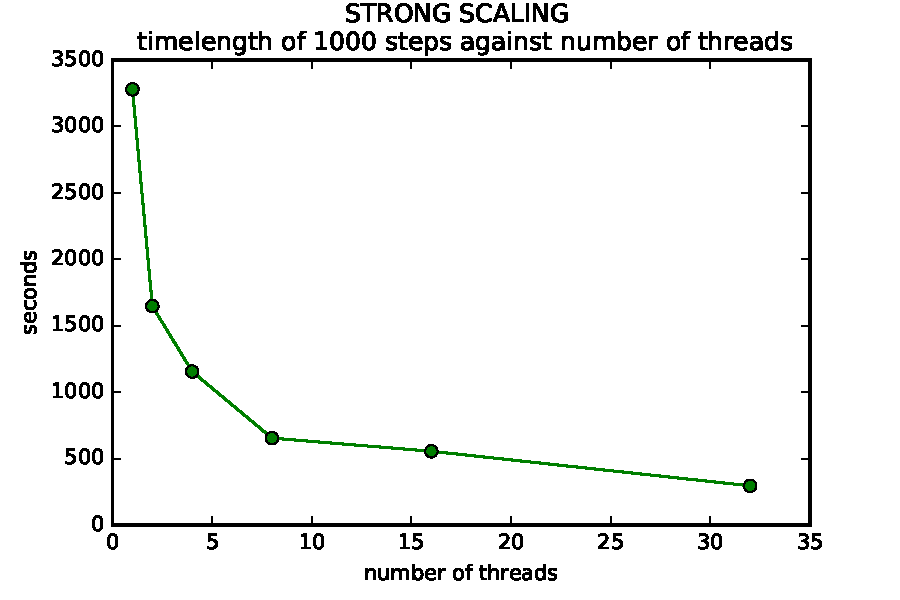
\includegraphics[width=1\textwidth]{./img/strongscalingg}
\end{figure}

For the weak scaling, the diameter of the sphere varied, so that the volume of lattice was increasing proportionally to the number of threads. However, side of the lattice must be multiple of $10$, because macroscopic velocity is computed over the cube with side of $10$. Therefore, the number of nodes per one thread slightly differs -- by no more then $5\%$ at most.

\begin{tabular}{ |p{2cm}|p{4cm}|p{4cm}| }
 \hline
 Threads & Diameter [nodes] & Nodes per one thread \\
 \hline
 \hline
$1$ & $320$ & $32\,768\,000$ \\
 \hline
$2$ & $400$ & $32\,000\,000$\\
 \hline
$4$ & $500$ & $31\,250\,000$ \\
 \hline
$8$ & $630$ & $31\,255\,875$\\
 \hline
$16$ & $800$ & $32\,000\,000$ \\
 \hline
$32$ & $1000$ & $31\,250\,000$ \\
 \hline
 \end{tabular}


\begin{figure}[H]
 \centering 
 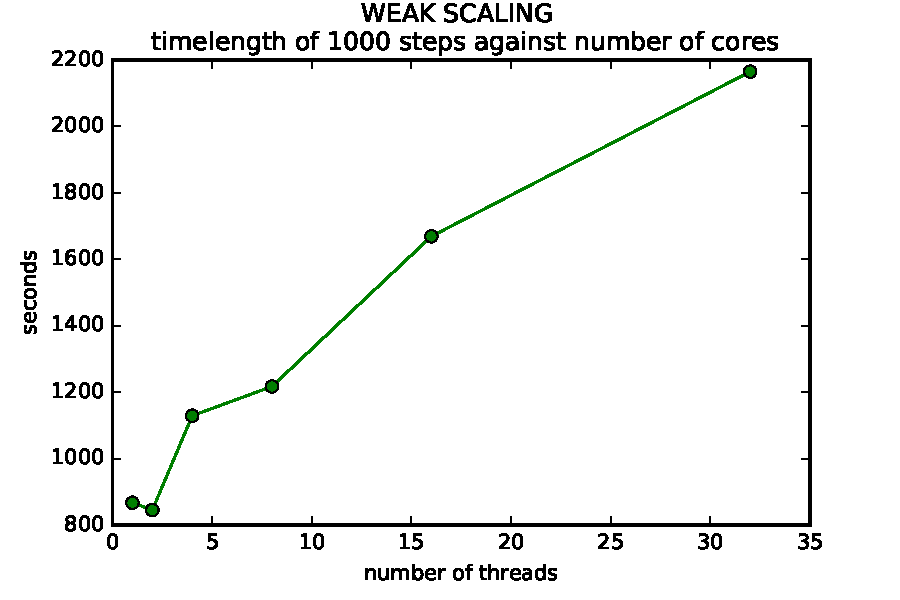
\includegraphics[width=1\textwidth]{./img/weakscaling}
\end{figure}

All computations were performed on the cluster Alfrid of University of West Bohemia.

\begin{tabular}{ |p{4cm}|p{8.8cm}| }
\hline
\multicolumn{2}{|c|}{Alfrid cluster} \\
\hline
\hline
Architecture &          x$86\_64$ \\
\hline
CPU op-mode(s) &        32-bit, 64-bit \\
\hline
Byte Order &            Little Endian \\
\hline
CPU(s) &                32 \\
\hline
On-line CPU(s) list &   0-31 \\
\hline
Thread(s) per core &    2 \\
\hline
Core(s) per socket &    8 \\
\hline
Socket(s) &             2 \\
\hline
NUMA node(s) &          2 \\
\hline
Vendor ID &             GenuineIntel \\
\hline
CPU family &            6 \\
\hline
Model &                 62 \\
\hline
Model name &            Intel(R) Xeon(R) CPU E5-2650 v2 @ 2.60GHz \\
\hline
Stepping &              4 \\
\hline
CPU MHz &               1216.007 \\
\hline
CPU max MHz &           3400.0000 \\
\hline
CPU min MHz &           1200.0000 \\
\hline
BogoMIPS &              5201.43 \\
\hline
Virtualization &        VT-x \\
\hline
L1d cache &            32K \\
\hline
L1i cache &            32K \\
\hline
L2 cache &            256K \\
\hline
L3 cache &              20480K \\
\hline
NUMA node0 CPU(s) &     0-7,16-23 \\
\hline
NUMA node1 CPU(s) &     8-15,24-31 \\
 \hline
 \end{tabular}


\chapter{Practical part}

%Short review of what follows:
In the theoretical part of the thesis, we have introduced the notion of cellular automaton and basic models of lattice-gas cellular automata by which it is possible to mimic the flow of physical fluids governed by the Euler equations and, to certain extent, the Navier-Stokes equations.
We have described the algorithms behind the microdynamics of these models and emphasized the importance of the symmetries of the lattice for reproducing correct macroscopic behavior.

In this part, we implement the aforementioned algorithms in the language C++ and visualize the results using the \textit{GNU}plot software. The original results of this thesis are summarized in the points to follow.



\begin{enumerate}
\item We implemented Turing-complete 1D and 2D cellular automata to show their interesting properties and motivate theoretical part. These results were already included in the theoretical part and will not be discussed further.
\item We implement FCHC and PI -- the two distinct 3D LGCA introduced in theoretical part.
\item We inspect 3D flow around obstacles of various shapes.
\item We study fully-developed turbulent flow and compare its statistical pro\-perties to the Kolmogorov--Obuchov K41 theory. \cite{wolf}.

Unfortunately, this most original and scientifically most interesting part is not concluded, but it provides the basis for future research. 

\end{enumerate}

%\include{Paral}
\chapter{Implementation}

According to \cite{wolf}, the most effective language for the implementation of LGCA is C, with slightly better performance than Fortran.
In our implementation, we could not resist to use some comfortable features of C++, but we have sticked to the low-level C-style of programming.
\bigskip

%We listened to this advice and started the implementation in C language, but we could not resist to use some "shortcuts" of C++, but we stayed true to the C-style of programming.
%
%\bigskip

%The programs have substantially grew over the time, and in case of further development,

%and we got on the crossroad how to efficiently develop our two models further. The current option number one (in the process while writing these lines) is to use the pure C, and pack it as \textit{extension module} to Python, mainly for our own comfort in future applications, but we would be glad if it finds its way to some fellow out there.

\section{Parallelization}
Languages C and C++ offer three widely used interfaces for parallelization:
\begin{enumerate}
\item OpenMP
\item MPI
\item Cuda
\end{enumerate}
%
%We rather obey the old Chinese saying 
%\begin{CJK*}{UTF8}{gbsn}
%'谁闻起来像腋下汗湿的龙,不应该使用 Cuda', so Cuda is obviously out of the question.
%\end{CJK*}

\bigskip

MPI was our hot candidate from the beginning, we have even used it on the cellular automaton not included in this thesis. 
%But after consulting the experienced colleague, we concluded that OpenMP would be more appropriate choice.
But in the end, we concluded that OpenMP would be more appropriate choice.
Since we have opporunity to use clusters at Metacenter (the network of academic clusters all over the Czech republic) we expected we could employ huge amount of processors, if we use MPI and compute on various clusters parallely. But we learnt that in the practice we can hardly employ more then two hundreds of processors.
Using OpenMP, we can run the computation on SMP machine with 64 processors, which is not significantly lower.

The drawbacks of MPI are obvious, it requires vast modification of the code, comparing to OpenMP, that usually requires only several lines of code to add.

Moreover, parallelization with OpenMP can be easily included to Python extension module, in case we decide to develop it.

In the following section, we provide a useful measure of our parallel implementation, the \textit{scaling efficiency}. It indicates the speedup of the computation with the increasing number of processing units employed.
We use two distinct ideas of scaling efficiency.

\section{Strong scaling}
In strong scaling measurement, we vary the number of processing units, while the problem size stays fixed.

The formula is as simple as
\begin{align*}
s_N = \frac{t_1}{N t_N} 100\%,
\end{align*}
where $t_1$ is a time to finish the work with one processing unit and $t_N$ is time to finish the same amount of work with $N$ processing units.

The idea of strong scaling is to find a "sweet spot" -- optimal number of computational units to compensate for the overhead of parrallelisation.
%relative to the overhead ...
\section{Weak scaling}
In this measurement, we vary number of processing units, but we vary also the size of the problem accordingly, so that amount of work per one processing unit is constant.

The weak scaling formula reads
\begin{align*}
w_N = \frac{t_1}{t_N} 100\%,
\end{align*}
where $t_1$ is time to complete $1$ unit of workload with $1$ processing unit, while $t_N$ is time to complete $N$ units of workload with $N$ processing units.

Therefore, the weak scaling tells us how requirements on memory bandwidth and other resources depend on the size of the problem.

\section{Flow on the sphere}
The most time--consuming simulation that we performed was the turbulent flow inside the sphere simulated by Pair-interaction, so the measurement of scaling on this problem is of the highest importance.

The strong scaling was measured on the sphere with diameter $d = 500$ over $3000$ time-steps.
On the graph below, we plotted time--length of the last $1000$ steps against the number of cores employed.
\begin{figure}[H]
 \centering 
 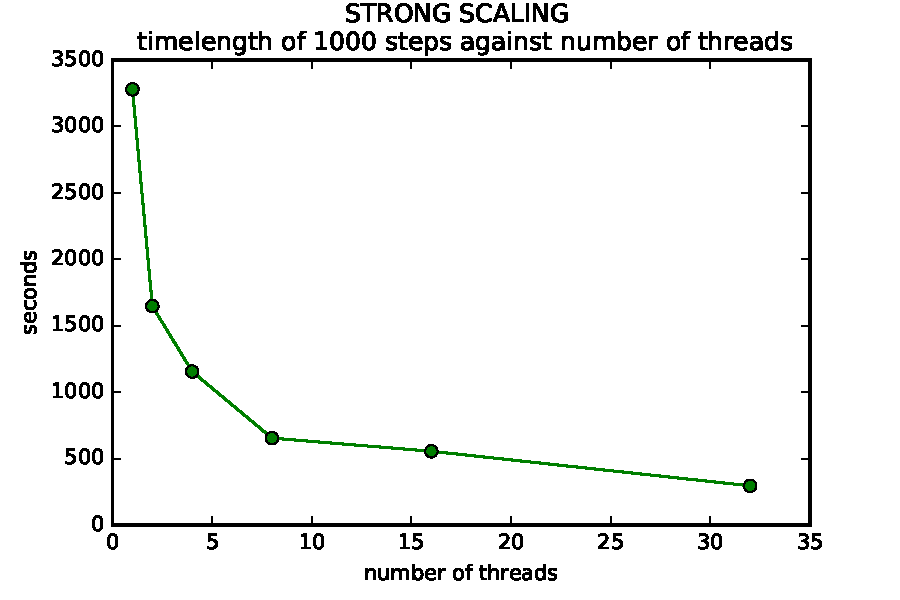
\includegraphics[width=1\textwidth]{./img/strongscalingg}
\end{figure}

For the weak scaling, the diameter of the sphere varied, so that the volume of lattice was increasing proportionally to the number of threads. However, side of the lattice must be multiple of $10$, because macroscopic velocity is computed over the cube with side of $10$. Therefore, the number of nodes per one thread slightly differs -- but no more then $5\%$.

\begin{tabular}{ |p{2cm}|p{4cm}|p{4cm}| }
 \hline
 Threads & Diameter [nodes] & Nodes per one thread \\
 \hline
 \hline
$1$ & $320$ & $32\,768\,000$ \\
 \hline
$2$ & $400$ & $32\,000\,000$\\
 \hline
$4$ & $500$ & $31\,250\,000$ \\
 \hline
$8$ & $630$ & $31\,255\,875$\\
 \hline
$16$ & $800$ & $32\,000\,000$ \\
 \hline
$32$ & $1000$ & $31\,250\,000$ \\
 \hline
 \end{tabular}


\begin{figure}[H]
 \centering 
 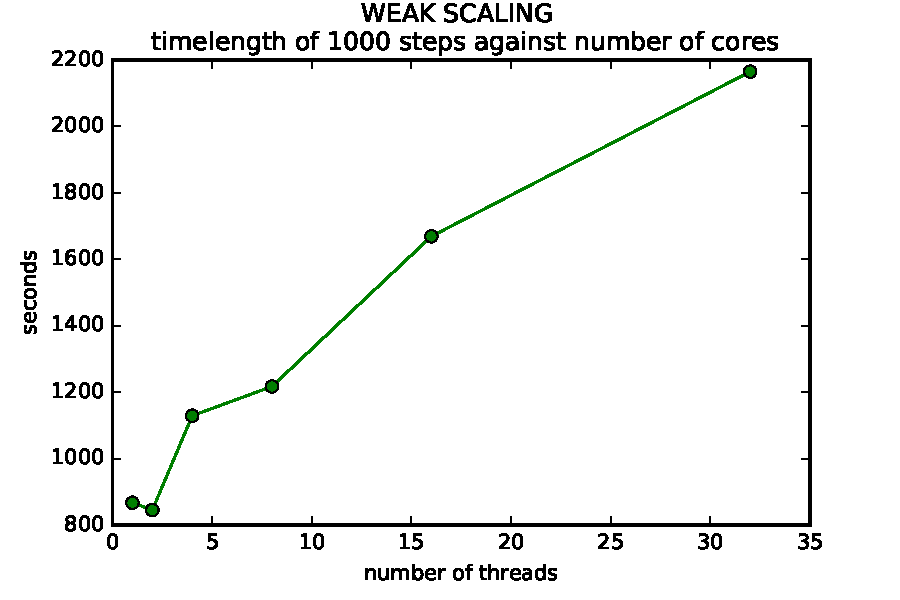
\includegraphics[width=1\textwidth]{./img/weakscaling}
\end{figure}

All computations were performed on the cluster \textbf{Alfrid} of \textit{University of West Bohemia}.

\begin{tabular}{ |p{4cm}|p{8.8cm}| }
\hline
\multicolumn{2}{|c|}{Alfrid cluster} \\
\hline
\hline
Architecture &          x$86\_64$ \\
\hline
CPU op-mode(s) &        32-bit, 64-bit \\
\hline
Byte Order &            Little Endian \\
\hline
CPU(s) &                32 \\
\hline
On-line CPU(s) list &   0-31 \\
\hline
Thread(s) per core &    2 \\
\hline
Core(s) per socket &    8 \\
\hline
Socket(s) &             2 \\
\hline
NUMA node(s) &          2 \\
\hline
Vendor ID &             GenuineIntel \\
\hline
CPU family &            6 \\
\hline
Model &                 62 \\
\hline
Model name &            Intel(R) Xeon(R) CPU E5-2650 v2 @ 2.60GHz \\
\hline
Stepping &              4 \\
\hline
CPU MHz &               1216.007 \\
\hline
CPU max MHz &           3400.0000 \\
\hline
CPU min MHz &           1200.0000 \\
\hline
BogoMIPS &              5201.43 \\
\hline
Virtualization &        VT-x \\
\hline
L1d cache &            32K \\
\hline
L1i cache &            32K \\
\hline
L2 cache &            256K \\
\hline
L3 cache &              20480K \\
\hline
NUMA node0 CPU(s) &     0-7,16-23 \\
\hline
NUMA node1 CPU(s) &     8-15,24-31 \\
 \hline
 \end{tabular}

%In the following chapter, we offer brief discussion of the most important parts of our source code.
\chapter{Implementation of FCHC}

In the chapter $3$ and $4$, we theoretically analyzed FCHC automaton and explained its collision algorithm proposed by Henon. In this chapter, we briefly comment on our implementation.

%Not so long ago, table that would specify collision rules for $2^{24}$ states was problematic - it would require approximately $2^{24} \cross 10 \cross 4 bytes = 640$MB memory to manage.
%
%Henon proposed algorithm for collision that would by-pass this obstacle, compute the possible set of states in reasonable time and chose optimal state.

%This algorithm is very expensive on computation time, especially comparing to pair-interaction LGCA.


\begin{enumerate}
\item Before the simulation of the flow starts, we compute the table with $2^{24}$ rows. Integer index of the row in the table is the state of the node. Using Henon's algorithm, we compute the optimal isometries for each state.
\item Collisions are resolved by choosing random optimal state from the table, instead of computing the optimal isometries during collision. To avoid overhead of the random numbers generator, we were choosing optimal states one after another, so that each state is used with the same frequency.
%
%We are not generating the random numbers to chose the resulting state, as it is expensive on resources and was significantly slowing the algorithm in the testing phase. However, we believe that choosing random states is not necessary and our solution for choosing the optimal isometries leads to the uniform distribution due to large number of nodes (around $10^{8}$).
\end{enumerate}

Excerpts of the source code for the computation of table would span $700$ lines of text, so we do not show it here. As all source code presented in this chapter, it can be found in \url{https://github.com/tuniak/fchc}.
%\section{Algorithm for the creation of the table}
%\begin{lstlisting}
%/* The node is represented as the integer, first 24 bits corresponds to the cells. If the value of the cell is 1, it is occupied by particle, otherwise it is 0. */
%   
%#define C1 1
%#define C2 (C1<<1)
%#define C3 (C1<<2)
%#define C4 (C1<<3)
%#define C5 (C1<<4)
%#define C6 (C1<<5)
%#define C7 (C1<<6)
%#define C8 (C1<<7)
%#define C9 (C1<<8)
%#define C10 (C1<<9)
%#define C11 (C1<<10)
%#define C12 (C1<<11)
%#define C13 (C1<<12)
%#define C14 (C1<<13)
%#define C15 (C1<<14)
%#define C16 (C1<<15)
%#define C17 (C1<<16)
%#define C18 (C1<<17)
%#define C19 (C1<<18)
%#define C20 (C1<<19)
%#define C21 (C1<<20)
%#define C22 (C1<<21)
%#define C23 (C1<<22)
%#define C24 (C1<<23)
%
%/* We assigned the 25th bit to the obstacle. If it is 1, this node is part of the obstacle and is not occupied by the particles (thus if this bit is 1, all other bits are 0) */
%#define OBS (C1<<24)
%
%/* We create the array of the cells, so we can efficiently iterate over the cells */
%int C[24] = {
%	C1,  C2,  C3,  C4,
%	C5,  C6,  C7,  C8,
%	C9,  C10, C11, C12,
%	C13, C14, C15, C16,
%	C17, C18, C19, C20,
%	C21, C22, C23, C24
%};
%
%/* Array of the cells, such that Reverse[i] lies on the diagonal to the C[i] */
%int Reverse[24] = {
%	C4, C3, C2, C1,
%	C8, C7, C6, C5,
%	C12,C11,C10,C9,
%	C16,C15,C14,C13,
%	C20,C19,C18,C17,
%	C24,C23,C22,C21
%};
%
%/* Lattice velocities. The lattice velocity c[i] corresponds to the cell C[i] */
%const int c[24][4] = {
%	{ 1,1,0,0 },
%	{ 1,-1,0,0 },
%	{ -1,1,0,0 },
%	{ -1,-1,0,0 },
%	
%	{ 1,0,1,0 },
%	{ 1,0,-1,0 },
%	{ -1,0,1,0 },
%	{ -1,0,-1,0 },
%
%	{ 1,0,0,1 },
%	{ 1,0,0,-1 },
%	{ -1,0,0,1 },
%	{ -1,0,0,-1 },
%
%	{ 0,1,1,0 },
%	{ 0,1,-1,0 },
%	{ 0,-1,1,0 },
%	{ 0,-1,-1,0 },
%
%	{ 0,1,0,1 },
%	{ 0,1,0,-1 },
%	{ 0,-1,0,1 },
%	{ 0,-1,0,-1 },
%
%	{ 0,0,1,1 },
%	{ 0,0,1,-1 },
%	{ 0,0,-1,1 },
%	{ 0,0,-1,-1 }
%};
%
%/* This function swap the i-th and j-th bit of the node n */
%int switchBits(int n, int i, int j)
%{
%	int a, b;
%	a = n & C[i];
%	b = n & C[j];
%	if (a > 0 && b == 0)
%	{
%		n ^= C[i];
%		n |= C[j];
%	}
%	else if (b > 0 && a == 0)
%	{
%		n |= C[i];
%		n ^= C[j];
%	}
%	return n;
%}
%
%/* Implementation of the isometries \Sigma_1 and \Sigma_2 on the node n*/
%/* As all isometries that will follow, it is achieved by swapping the appropriate bits in the node */
%/* It also transforms the momentum vector q */
%/* The parameter j is dummy parameter, we need it so that all isometries have the same set of parameters */
%int sigma(int n, int* q, int i, int j)
%{
%	int a = q[0];
%	int b = q[1];
%	int c = q[2];
%	int d = q[3];
%
%	if (i == 1)
%	{
%		q[0] = ( a + b + c - d ) / 2;
%		q[1] = ( a + b - c + d ) / 2;
%		q[2] = ( a - b + c + d ) / 2;
%		q[3] = (-a + b + c + d ) / 2;
%
%		n = switchBits(n, 1, 21);
%		n = switchBits(n, 2, 22);
%		n = switchBits(n, 5, 17);
%		n = switchBits(n, 6, 18);
%		n = switchBits(n, 8, 12);
%		n = switchBits(n, 11, 15);
%	}
%	else
%	{
%		q[0] = ( a + b + c + d ) / 2;
%		q[1] = ( a + b - c - d ) / 2;
%		q[2] = ( a - b + c - d ) / 2;
%		q[3] = ( a - b - c + d ) / 2;
%
%		n = switchBits(n, 1, 20);
%		n = switchBits(n, 2, 23);
%		n = switchBits(n, 5, 16);
%		n = switchBits(n, 6, 19);
%		n = switchBits(n, 9, 12);
%		n = switchBits(n, 10, 15);
%	}
%	return n;
%}
%
%/* Isometry S_i is the reflection over plane x_i */
%int S(int n, int* q, int i, int j)
%{
%	switch (i)
%	{
%	case 1:
%		q[0] = -q[0];
%		n = switchBits(n, 0, 2);
%		n = switchBits(n, 1, 3);
%		n = switchBits(n, 4, 6);
%		n = switchBits(n, 5, 7);
%		n = switchBits(n, 8, 10);
%		n = switchBits(n, 9, 11);
%		break;
%	case 2:
%		q[1] = -q[1];
%		n = switchBits(n, 0, 1);
%		n = switchBits(n, 2, 3);
%		n = switchBits(n, 12, 14);
%		n = switchBits(n, 13, 15);
%		n = switchBits(n, 16, 18);
%		n = switchBits(n, 17, 19);
%		break;
%	case 3:
%		q[2] = -q[2];
%		n = switchBits(n, 4, 5);
%		n = switchBits(n, 6, 7);
%		n = switchBits(n, 12, 13);
%		n = switchBits(n, 14, 15);
%		n = switchBits(n, 20, 22);
%		n = switchBits(n, 21, 23);
%		break;
%	case 4:
%		q[3] = -q[3];
%		n = switchBits(n, 8, 9);
%		n = switchBits(n, 10, 11);
%		n = switchBits(n, 16, 17);
%		n = switchBits(n, 18, 19);
%		n = switchBits(n, 20, 21);
%		n = switchBits(n, 22, 23);
%		break;
%	default:
%		break;
%	}
%	return n;
%}
%
%/* Isometry P_ij, reflecton over the plain x_i = x_j */
%int P(int n, int*q, int i, int j)
%{
%	int a = i - 1;
%	int b = j - 1;
%	int qa = q[a];
%	q[a] = q[b];
%	q[b] = qa;
%
%	if (i == 1)
%	{
%		if (j == 2)
%		{
%			n = switchBits(n, 1, 2);
%			n = switchBits(n, 4, 12);
%			n = switchBits(n, 5, 13);
%			n = switchBits(n, 6, 14);
%			n = switchBits(n, 7, 15);
%			n = switchBits(n, 8, 16);
%			n = switchBits(n, 9, 17);
%			n = switchBits(n, 10, 18);
%			n = switchBits(n, 11, 19);
%		}
%		else if (j == 3)
%		{
%			n = switchBits(n, 0, 12);
%			n = switchBits(n, 1, 14);
%			n = switchBits(n, 2, 13);
%			n = switchBits(n, 3, 15);
%			n = switchBits(n, 5, 6);
%			n = switchBits(n, 8, 20);
%			n = switchBits(n, 9, 21);
%			n = switchBits(n, 10, 22);
%			n = switchBits(n, 11, 23);
%		}
%		else if (j == 4)
%		{
%			n = switchBits(n, 0, 16);
%			n = switchBits(n, 1, 18);
%			n = switchBits(n, 2, 17);
%			n = switchBits(n, 3, 19);
%			n = switchBits(n, 4, 20);
%			n = switchBits(n, 5, 22);
%			n = switchBits(n, 6, 21);
%			n = switchBits(n, 7, 23);
%			n = switchBits(n, 9, 10);
%		}
%	}
%	else if (i == 2)
%	{
%		if (j == 3)
%		{
%			n = switchBits(n, 0, 4);
%			n = switchBits(n, 1, 5);
%			n = switchBits(n, 2, 6);
%			n = switchBits(n, 3, 7);
%			n = switchBits(n, 13, 14);
%			n = switchBits(n, 16, 20);
%			n = switchBits(n, 17, 21);
%			n = switchBits(n, 18, 22);
%			n = switchBits(n, 19, 23);
%		}
%		else if (j == 4)
%		{
%			n = switchBits(n, 0, 8);
%			n = switchBits(n, 1, 9);
%			n = switchBits(n, 2, 10);
%			n = switchBits(n, 3, 11);
%			n = switchBits(n, 12, 20);
%			n = switchBits(n, 13, 22);
%			n = switchBits(n, 14, 21);
%			n = switchBits(n, 15, 23);
%			n = switchBits(n, 17, 18);
%		}
%	}
%	else if (i == 3 && j == 4)
%	{
%		n = switchBits(n, 4, 8);
%		n = switchBits(n, 5, 9);
%		n = switchBits(n, 6, 10);
%		n = switchBits(n, 7, 11);
%		n = switchBits(n, 12, 16);
%		n = switchBits(n, 13, 17);
%		n = switchBits(n, 14, 18);
%		n = switchBits(n, 15, 19);
%		n = switchBits(n, 21, 22);
%	}
%	return n;
%}
%
%/* Computes the total momentum of the node */
%int* momenta(int node)
%{
%	int*q = new int[4]{ 0,0,0,0 };
%
%	for (int i = 0; i < 24; ++i)
%	{
%		/* if the cell C[i] is occupied by particle, count its momentum */
%		if (C[i] & node)
%		{
%			for (int j = 0; j < 4; ++j)
%			{
%				q[j] += c[i][j];
%			}
%		}
%	}
%	return q;
%}
%
%/* We need to remember all the isometries that normalize the momentum, so we can transform it back to its original momentum */
%/* We define this array so that we can reffer to the isometry by the single index */
%int(*iso[])(int n, int*q, int i, int j) = { S,P,sigma };
%
%/* This function does all isometries that normalized the node, but in the reverse order, so that original momentum is achieved */
%void goBack(int**steps, int* nodes, int*q, int step, int length)
%{
%	for (int i = 1; i < length; i++)
%	{
%		for (int j = step - 1; j >= 0; --j)
%		{
%			nodes[i] = iso[steps[j][0]](nodes[i], q, steps[j][1], steps[j][2]);
%		}
%	}
%}
%
%/* Creates the entry for the state 'n' that we will insert into the table of collisions */
%/* It is implementation of the Henon algorithm, that computes the set of optimal isometries */ 
%int* newNode(int n, int**steps)
%{
%	int*q = momenta(n);
%
%	int step = 0;
%	
%	// invert negative q[i]
%	for (int i = 0; i < 4; i++)
%	{
%		if (q[i] < 0)
%		{
%			//S changes sign of q[i];
%			n = S(n, q, i+1, 0);
%			//we record each step to the array "steps" so we can go back
%			steps[step][0] = 0;
%			steps[step][1] = i+1;
%			steps[step][2] = 0;
%			++step;
%		}
%	}
%	// sort q[i] from high to low
%	int highIndex;
%	int highValue;
%	for (int i = 0; i < 4; ++i)
%	{
%		highIndex = i;
%		highValue = q[i];
%		for (int j = i+1; j < 4; ++j)
%		{
%			if (q[j] > highValue)
%			{
%				highValue = q[j];
%				highIndex = j;
%			}
%		}
%		if (highIndex > i)
%		{
%			n = P(n, q, i + 1, highIndex + 1);
%			steps[step][0] = 1;
%			steps[step][1] = i + 1;
%			steps[step][2] = highIndex + 1;
%			++step;
%		}
%	}
%	// to fulfill second condition:
%	if (q[3] > 0)
%	{
%		if (q[0] + q[3] == q[1] + q[2])
%		{
%			n = sigma(n, q, 2, 0);
%			steps[step][0] = 2;
%			steps[step][1] = 2;
%			steps[step][2] = 0;
%			++step;
%		}
%		else if (q[0] + q[3] > q[1] + q[2])
%		{
%			n = sigma(n, q, 1, 0);
%			steps[step][0] = 2;
%			steps[step][1] = 1;
%			steps[step][2] = 0;
%			++step;
%		}
%	}
%	if (q[3] < 0)
%	{
%		n = S(n, q, 4, 0);
%		//we record each step to the steps field, since we will go back
%		steps[step][0] = 0;
%		steps[step][1] = 4;
%		steps[step][2] = 0;
%		++step;
%	}
%
%	int* nodes;
%	//class 12
%	if (q[0] == 0)
%	{
%		int length = 13;
%		nodes = new int[length];
%		nodes[0] = length - 1;
%		//S3 S1 P34 P12,  S4 S1 P34 P12,  S3 S2 P34 P12, S4 S2 P34 P12,  
%		//S2 S1 P24 P13,  S4 S1 P24 P13,  S3 S2 P24 P13, S4 S3 P24 P13,
%		//S2 S1 P23 P14,  S3 S1 P23 P14,  S4 S2 P23 P14, S4 S3 P23 P14
%
%		nodes[1] = P(n, q, 1, 2);
%		nodes[1] = P(nodes[1], q, 3, 4);
%		nodes[1] = S(nodes[1], q, 1, 0);
%		nodes[1] = S(nodes[1], q, 3, 0);
%
%		nodes[2] = P(n, q, 1, 2);
%		nodes[2] = P(nodes[2], q, 3, 4);
%		nodes[2] = S(nodes[2], q, 1, 0);
%		nodes[2] = S(nodes[2], q, 4, 0);
%
%		nodes[3] = P(n, q, 1, 2);
%		nodes[3] = P(nodes[3], q, 3, 4);
%		nodes[3] = S(nodes[3], q, 2, 0);
%		nodes[3] = S(nodes[3], q, 3, 0);
%
%		nodes[4] = P(n, q, 1, 2);
%		nodes[4] = P(nodes[4], q, 3, 4);
%		nodes[4] = S(nodes[4], q, 2, 0);
%		nodes[4] = S(nodes[4], q, 4, 0);
%
%		nodes[5] = P(n, q, 1, 3);
%		nodes[5] = P(nodes[5], q, 2, 4);
%		nodes[5] = S(nodes[5], q, 1, 0);
%		nodes[5] = S(nodes[5], q, 2, 0);
%
%		nodes[6] = P(n, q, 1, 3);
%		nodes[6] = P(nodes[6], q, 2, 4);
%		nodes[6] = S(nodes[6], q, 1, 0);
%		nodes[6] = S(nodes[6], q, 4, 0);
%
%		nodes[7] = P(n, q, 1, 3);
%		nodes[7] = P(nodes[7], q, 2, 4);
%		nodes[7] = S(nodes[7], q, 2, 0);
%		nodes[7] = S(nodes[7], q, 3, 0);
%
%		nodes[8] = P(n, q, 1, 3);
%		nodes[8] = P(nodes[8], q, 2, 4);
%		nodes[8] = S(nodes[8], q, 3, 0);
%		nodes[8] = S(nodes[8], q, 4, 0);
%
%		nodes[9] = P(n, q, 1, 4);
%		nodes[9] = P(nodes[9], q, 2, 3);
%		nodes[9] = S(nodes[9], q, 1, 0);
%		nodes[9] = S(nodes[9], q, 2, 0);
%		
%		nodes[10] = P(n, q, 1, 4);
%		nodes[10] = P(nodes[10], q, 2, 3);
%		nodes[10] = S(nodes[10], q, 1, 0);
%		nodes[10] = S(nodes[10], q, 3, 0);
%
%		nodes[11] = P(n, q, 1, 4);
%		nodes[11] = P(nodes[11], q, 2, 3);
%		nodes[11] = S(nodes[11], q, 2, 0);
%		nodes[11] = S(nodes[11], q, 4, 0);
%
%		nodes[12] = P(n, q, 1, 4);
%		nodes[12] = P(nodes[12], q, 2, 3);
%		nodes[12] = S(nodes[12], q, 3, 0);
%		nodes[12] = S(nodes[12], q, 4, 0);
%
%		goBack(steps, nodes, q, step, length);
%	}
%	//class 11
%	else if (q[1] == 0)
%	{
%		int length = 7;
%		nodes = new int[length];
%		nodes[0] = length - 1;
%		//S4 S2 P23,   S4 S3 P23,   S3 S2 P24,   
%		//S4 S3 P24,   S3 S2 P34,   S4 S2 P34
%
%		nodes[1] = P(n, q, 2, 3);
%		nodes[1] = S(nodes[1], q, 2, 0);
%		nodes[1] = S(nodes[1], q, 4, 0);
%
%		nodes[2] = P(n, q, 2, 3);
%		nodes[2] = S(nodes[2], q, 3, 0);
%		nodes[2] = S(nodes[2], q, 4, 0);
%
%		nodes[3] = P(n, q, 2, 4);
%		nodes[3] = S(nodes[3], q, 2, 0);
%		nodes[3] = S(nodes[3], q, 3, 0);
%
%		nodes[4] = P(n, q, 2, 4);
%		nodes[4] = S(nodes[4], q, 3, 0);
%		nodes[4] = S(nodes[4], q, 4, 0);
%
%		nodes[5] = P(n, q, 3, 4);
%		nodes[5] = S(nodes[5], q, 2, 0);
%		nodes[5] = S(nodes[5], q, 3, 0);
%
%		nodes[6] = P(n, q, 3, 4);
%		nodes[6] = S(nodes[6], q, 2, 0);
%		nodes[6] = S(nodes[6], q, 4, 0);
%		
%		goBack(steps, nodes, q, step, length);
%	}
%	//class 10
%	else if (q[2] == 0 && q[0]==q[1])
%	{
%		int length = 7;
%		nodes = new int[length];
%		nodes[0] = length - 1;
%		//S3,P34,P12,   S4,P34,P12,   S4,S3,sigma1,   S4,S3,P34,P12,sigma1
%		//S4,S3,sigma2,   P34,P12,sigma2
%		nodes[1] = P(n, q, 1, 2);
%		nodes[1] = P(nodes[1], q, 3, 4);
%		nodes[1] = S(nodes[1], q, 3, 0);
%
%		nodes[2] = P(n, q, 1, 2);
%		nodes[2] = P(nodes[2], q, 3, 4);
%		nodes[2] = S(nodes[2], q, 4, 0);
%
%		nodes[3] = sigma(n, q, 1, 0);
%		nodes[3] = S(nodes[3], q, 3, 0);
%		nodes[3] = S(nodes[3], q, 4, 0);
%
%		nodes[4] = sigma(n, q, 1, 0);
%		nodes[4] = P(nodes[4], q, 1, 2);
%		nodes[4] = P(nodes[4], q, 3, 4);
%		nodes[4] = S(nodes[4], q, 3, 0);
%		nodes[4] = S(nodes[4], q, 4, 0);
%
%		nodes[5] = sigma(n, q, 2, 0);
%		nodes[5] = S(nodes[5], q, 3, 0);
%		nodes[5] = S(nodes[5], q, 4, 0);
%
%		nodes[6] = sigma(n, q, 2, 0);
%		nodes[6] = P(nodes[6], q, 1, 2);
%		nodes[6] = P(nodes[6], q, 3, 4);
%
%		goBack(steps, nodes, q, step, length);
%	}
%	//class 9
%	else if (q[2] == 0 && q[0] > q[1])
%	{
%		int length = 4;
%		nodes = new int[length];
%		nodes[0] = length - 1;
%		
%		nodes[1] = S(n, q, 3, 0);
%		nodes[1] = S(nodes[1], q, 4, 0);
%		
%		nodes[2] = P(n, q, 3, 4);
%		nodes[2] = S(nodes[2], q, 3, 0);
%		
%		nodes[3] = P(n, q, 3, 4);
%		nodes[3] = S(nodes[3], q, 4, 0);
%
%		goBack(steps, nodes, q, step, length);
%	}
%	//class 8
%	else if (q[0]==q[1] && q[1] == q[2] && q[2] > q[3] && q[3]==0)
%	{
%		int length = 5;
%		nodes = new int[length];
%		nodes[0] = length - 1;
%		//1
%		nodes[1] = P(n, q, 1, 2);
%		nodes[1] = P(nodes[1], q, 2, 3);
%		//2
%		nodes[2] = P(n, q, 1, 3);
%		nodes[2] = P(nodes[2], q, 2, 3);
%		//3
%		nodes[3] = P(n, q, 1, 2);
%		nodes[3] = P(nodes[3], q, 2, 3);
%		nodes[3] = S(nodes[3], q, 4, 0);
%
%		//4
%		nodes[4] = P(n, q, 1, 3);
%		nodes[4] = P(nodes[4], q, 2, 3);
%		nodes[4] = S(nodes[4], q, 4, 0);
%
%		goBack(steps, nodes, q, step, length);
%	}
%	//class 6 or 7
%	else if (q[0]>q[1] && q[1]==q[2] && q[2] > q[3] && q[3] == 0)
%	{
%		//class 6
%		if (q[0] == 2*q[1])
%		{
%			int length = 5;
%			nodes = new int[length];
%
%			nodes[0] = length - 1;
%
%			nodes[1] = sigma(n, q, 1, 0);
%			nodes[1] = S(nodes[1], q, 4, 0);
%
%			nodes[2] = sigma(n, q, 2, 0);
%			nodes[2] = S(nodes[2], q, 4, 0);
%
%			nodes[3] = sigma(n, q, 1, 0);
%			nodes[3] = P(nodes[3], q, 2, 3);
%			nodes[3] = S(nodes[3], q, 4, 0);
%
%			nodes[4] = sigma(n, q, 2, 0);
%			nodes[4] = P(nodes[4], q, 2, 3);
%			nodes[4] = S(nodes[4], q, 4, 0);
%
%			goBack(steps, nodes, q, step, length);
%		}
%		//class 7
%		else
%		{
%			int length = 2;
%			nodes = new int[length];
%
%			nodes[0] = length - 1;
%
%			nodes[1] = P(n, q, 2, 3);
%			nodes[1] = S(nodes[1], q, 4, 0);
%
%			goBack(steps, nodes, q, step, length);
%		}		
%	}
%	//class 5
%	else if (q[0]==q[1] && q[1]>q[2] && q[2] > q[3] && q[4] == 0)
%	{
%		int length = 2;
%		nodes = new int[length];
%
%		nodes[0] = length - 1;
%		//1
%		nodes[1] = P(n, q, 1, 2);
%		nodes[1] = S(nodes[1], q, 4, 0);
%
%		goBack(steps, nodes, q, step, length);
%	}
%	//class 3,4
%	else if (q[0]>q[1] && q[1]>q[2] && q[2] > q[3] && q[3] == 0)
%	{
%		//class 3
%		if (q[0]==q[1]+q[2])
%		{
%			int length = 3;
%			nodes = new int[length];
%			
%			nodes[0] = length - 1;
%
%			nodes[1] = sigma(n, q, 1, 0);
%			nodes[1] = S(nodes[1], q, 4, 0);
%
%			nodes[2] = sigma(n, q, 2, 0);
%			nodes[2] = S(nodes[2], q, 4, 0);
%
%			goBack(steps, nodes, q, step, length);
%		}
%		//class 4
%		else
%		{
%			int length = 2;
%			nodes = new int[length];
%
%			nodes[0] = length - 1;
%
%			nodes[1] = S(n, q, 4, 0);
%
%			goBack(steps, nodes, q, step, length);
%		}
%	}
%	//class 2
%	else if (q[0]==q[1] && q[1]==q[2] && q[2]>q[3] && q[3]>0)
%	{
%		int length = 3;
%		nodes = new int[length];
%
%		nodes[0] = length - 1;
%
%		nodes[1] = P(n, q, 1, 2);
%		nodes[1] = P(nodes[1], q, 2, 3);
%
%		nodes[2] = P(n, q, 1, 3);
%		nodes[2] = P(nodes[2], q, 2, 3);
%
%		goBack(steps, nodes, q, step, length);
%	}
%	//class 1
%	else if (q[0]==q[1] && q[1]>q[2] && q[2] > q[3] && q[3] > 0)
%	{
%		int length = 2;
%		nodes = new int[length];
%
%		nodes[0] = length - 1;
%
%		nodes[1] = P(n, q, 1, 2);
%
%		goBack(steps, nodes, q, step, length);
%	}
%	else
%		nodes = nullptr;
%	return nodes;
%}
%
%/*  This is the high-level function that creates the table of isometries */
%/* For all 2^24 possible states of the node, it calls the function newNode and save the set of new states */
%void fillTable(int** table)
%{
%	int n;
%	
%	int ** steps = new int*[20];
%	for(int i = 0; i<20; ++i)
%	   steps[i] = new int[3];	
%
%	for ( n = 0; n < OBS; ++n)
%		table[n] = newNode(n, steps);
%}
%\end{lstlisting}

\section{Algorithm for collision}
Once we have the table specifying optimal isometrical states ready, the collision reduces to randomly choosing an optimal state from the table. To avoid an expensive generation of random numbers, we are alternating isometries one by one and so we cover all final states uniformly.

\begin{lstlisting}
/* For all nodes 'n' on the grid, this function looks in the table and choose from optimal final states */

void Collision(int***grid, int**table, int t, int X, int Y, int Z)
{
	int x,y,z;

	int n;
	int k;
#pragma omp parallel for private (x,y,z,n,k)
	for (x = 0; x < X; ++x)
		for (y = 0; y < Y; ++y)
			for (z = 0; z < Z; ++z)
			{
				//We find that node with position [x][y][y] on the grid is in the state n 
				n = grid[x][y][z];
				// If there is obstacle in the node, we skip it.
				if (n & OBS)
					break;
				/* k is initialized by the external parameter t,
				    and k is moduled by number of optimal isometries for the state n */
				k = (t % table[n][0]) + 1;
				
				// we assign the k-th optimal state to the node 
				grid[x][y][z] = table[n][k];
				
				//every step, we increment the external parameter, so we hopefully achieve the uniform distribution of k (there is huge number of nodes on the grid)
				++t;
			}
}
\end{lstlisting}

\section{Propagation in FCHC}
Although the collisions are resolved in the four dimensional space (and the particles are the four dimensional objects), the propagation is performed on the 3D projection of FCHC lattice \ref{fchc}.
%for the purpose of propagation, we can simply 'forget' its four-dimensional nature.

\begin{lstlisting}
/* 
The propagation is supposed to happen simultaneously in all nodes at once. Because it is performed sequentially in the computation, we need to propagate particles from the current array to a different one. Every time step, these two arrays alternate.
*/
void Propagation(int***from, int***to, int**table, int X, int Y, int Z)
{
	int x,y,z;
	int i;
	int n;
	int new_x, new_y, new_z;

#pragma omp parallel for private (n, new_x, new_y, new_z, x, y, z, i)
	for ( x = 0; x < X; ++x)
		for ( y = 0; y < Y; ++y)
			for ( z = 0; z < Z; ++z)
			{
				// The current state of the node at [x][y][z]				
				n = from[x][y][z];
				// We check every cell
				for ( i = 0; i < 24; ++i)
				{
					// If the cell C[i] is occupied by particle, we propagate it to the corresponding node. 
					if (n & C[i])
					{
						new_x = PeriodicBC(x + c[i][0], X);
						new_y = PeriodicBC(y + c[i][1], Y);
						new_z = PeriodicBC(z + c[i][2], Z);
						// If there is an obstacle in the node, particle's velocity is reversed.
						// e.g. particle with velocity [1,0,-1,0] gains velocity [-1,0,1,0] by the reflection from the obstacle
						// Hence, in the next step, it propagates to the node where it come from
						if (to[new_x][new_y][new_z] & OBS)
							to[new_x][new_y][new_z] |= Reverse[i];
						else
							to[new_x][new_y][new_z] |= C[i];
					}
				}
				from[x][y][z] = 0;
			}
}
\end{lstlisting}
\chapter{Implementation of the Pair-Interaction LGCA in 3D}


\begin{chapquote}{Donald Knuth, \textit{Structured programming with GoTo statement}}
"Programmers waste enormous amounts of time thinking about, or worrying about, the speed of noncritical parts of their programs, and these attempts at efficiency actually have a strong negative impact when debugging and maintenance are considered. We should forget about small efficiencies, say about 97\% of the time: premature optimization is the root of all evil. Yet we should not pass up our opportunities in that critical 3\%."
\end{chapquote}
%
%\epigraph{Programmers waste enormous amounts of time thinking about, or worrying about, the speed of noncritical parts of their programs, and these attempts at efficiency actually have a strong negative impact when debugging and maintenance are considered. We should forget about small efficiencies, say about 97\% of the time: premature optimization is the root of all evil. Yet we should not pass up our opportunities in that critical 3\%.}{Donald Knuth in "Structured programming with GoTo statement"}


%We followed best practices of in \cite{},
Inspired by this quote of Donald and Knuth and best programming practice presented in \cite{lbm} on Lattice-Boltzmann implementation, we attempted to implement critical functions \textit{collision} and \textit{propagations} efficiently.

The parts of the code that we present is already parallelized by OpenMP.

\section{Implementation of the collision algorithm}
\begin{lstlisting}
#define A 1
#define B 2
#define C 4
#define D 8
#define E 16
#define F 32
#define G 64
#define H 128

unsigned char cell[8] = {A, B, C, D, E, F, G, H};


/* Node consists of 8 mass bits (char m) and 3x8 momentum bits (char p[3]). If there is an obstacle in the node <=>  node.o == 1. */
typedef struct
{
	unsigned char m;
	unsigned char p[3];
	int o;
} Node;
// We access the bits of the of the node by bitwise AND opperation
//e.g. node.m & A == 1 means there is particle in the cell A
// 		node.p[1] & A == 0 means that these particle has no momentum in Y-direction

// 3 directions (X, Y, Z), 4 pair-interactions in each direction, 2 cells in each pair 
unsigned char Pair[3][4][2] = 
{
	{
		{A,E}, {B,F}, {C,G}, {D,H}
	},
	{
		{A,C}, {B,D}, {E,G}, {F,H}
	},
	{
		{A,B}, {C,D}, {E,F}, {G,H}
	}
};

// The collision algorithm
void collision(Node &node)
{
	//d,u ... index for downer and upper momentum
	int d; //index of momentum in direction of PI
	int u; //index of momentum orthogonal to direction of PI

	// l, r ... left/right cell in the pair
	// ml, mr ... mass bits in the pair
	// lu, ld, ri, ru, rd, ri ... momenta bits in the pair
	unsigned char l, r, ml, mr, lu, ld, ru, rd, li, ri;

	for (int i = 0; i < 3; ++i)
	{
		d = (i + 1) % 3;
		u = (i + 2) % 3;
		for (int j = 0; j < 4; ++j)
		{
			l = Pair[i][j][0];
			r = Pair[i][j][1];

			ml = node.m&l;
			mr = node.m&r;
			ld = node.p[d] & l;
			lu = node.p[u] & l;
			li = node.p[i] & l;
			rd = node.p[d] & r;
			ru = node.p[u] & r;
			ri = node.p[i] & r;

			/* PAIR INTERACTIONS */
			if (!ml && !mr)
				continue;
			if (ml && mr)
			{
				// alternate momenta in direction of the pair-interaction
				if (!ld && !rd)
				{
					node.p[d] |= l;
					node.p[d] |= r;
				}
				else if (ld && rd)
				{
					node.p[d] ^= l;
					node.p[d] ^= r;
				}
				// alternate momenta in all other directions
				if (lu && !ru)
				{
					node.p[u] ^= l;
					node.p[u] |= r;
				}
				else if (!lu && ru)
				{
					node.p[u] |= l;
					node.p[u] ^= r;
				}
				if (li && !ri)
				{
					node.p[i] ^= l;
					node.p[i] |= r;
				}
				else if (!li && ri)
				{
					node.p[i] |= l;
					node.p[i] ^= r;
				}
			}
			else if (!ml && !rd)
			{
				node.m |= l;
				node.m ^= r;
				if (ru)
				{
					node.p[u] |= l;
					node.p[u] ^= r;
				}
				if (ri)
				{
					node.p[i] |= l;
					node.p[i] ^= r;
				}					
			}
			else if (!mr && !ld)
			{
				node.m |= r;
				node.m ^= l;
				if (lu)
				{
					node.p[u] |= r;
					node.p[u] ^= l;
				}
				if (li)
				{
					node.p[i] |= r;
					node.p[i] ^= l;
				}
			}
		}
	}
}

// 'Collision' runs over the lattice and calls function 'collision' on each node. 
void Collision(Node***array, int X, int Y, int Z, int start)
{
	int x,y,z;

#pragma omp parallel for private (x,y,z)
	for (x = start; x < X; x+=2)
	{
		for(y = start; y < Y; y+=2)
		{
			for(z = start; z < Z; z+=2)
			{
				// if the node is obstacle, skip it
				if(array[x][y][z].o)
					continue;
				collision(array[x][y][z]);
			}
		}
	}
}
\end{lstlisting}


\section{Implementation of the Propagation}
%Before we comment on the implementation, we want to emphasize one of the strong sides of PI automaton.

%In FCHC, the lattice consisted of all the nodes with the discrete Cartesian coordinates (up to some upper boundary denoted by X, Y, Z).
%All of these nodes were interconnected and formed single lattice.

As we explained in the teoretical part, the PI-3D lattice splits into 4 sub-lattices, that are not connected. We are using only one of these sub-lattices. At even times $t=2,4,...$ only nodes with even indices are populated, and at odd times, nodes with odd indices are populated.

Theoretically, this setting provides that spurious Zannetti's invariants are not present (\cite{nasilowski}), practically, we can use single data structure for the lattice before and after propagation. Comparing to other lattices, this provides additional speed-up by lowering memory bandwidth and saving other resources.

The excerpts of the code governing Propagation follows. 
\begin{lstlisting}
/* Group of cells that propagates in positive X-direction, Y-direction and Z-direction. */
#define dirX (B+D+F+H)
#define dirY (E+F+G+H)
#define dirZ (A+B+E+F)
/* For example, because A & dirX == 0, particle from A propagates in negative X direction,
    but A & dirZ == 1, so it propagates in positive Z direction. */

/* At start == 0, particles are streamed from even nodes ([0,2,124]...) to odd nodes([1,1,123]...) 
   At start == 1, from odd to even nodes. */
void Propagation(Node***array, int X, int Y, int Z, int start)
{

#pragma omp parallel for
	for (int x = start; x < X; x += 2)
	{
		for (int y = start; y < Y; y += 2)
		{
			for (int z = start; z < Z; z += 2)
			{
				// for cells in the node
				for (int k = 1; k <= H; k <<= 1)
				{
					//if there is particle in the cell, we propagate it
					if (array[x][y][z].m & k)
					{
						// if particle from cell[c] propagates in positive direction of X
						int xN = k & dirX ? (x + 1) % X : (x - 1 + X) % X;
						int yN = k & dirY ? (y + 1) % Y : (y - 1 + Y) % Y;
						int zN = k & dirZ ? (z + 1) % Z : (z - 1 + Z) % Z;
						// else particle propagates in negative direction of x

#pragma omp atomic
						array[xN][yN][zN].m |= k & array[x][y][z].m;
#pragma omp atomic
						array[xN][yN][zN].p[0] |= k & array[x][y][z].p[0];
#pragma omp atomic
						array[xN][yN][zN].p[1] |= k & array[x][y][z].p[1];
#pragma omp atomic
						array[xN][yN][zN].p[2] |= k & array[x][y][z].p[2];
					}
				}
				//in the old array, we set the node to 0
				array[x][y][z].m = 0;
				array[x][y][z].p[0] = 0;
				array[x][y][z].p[1] = 0;
				array[x][y][z].p[2] = 0;
			}
		}
	}
}
\end{lstlisting}
\chapter{Non-deterministic PI}

Pair-Interaction that Nasilowski proposed is deterministic, and it might be considered to be its advantage. 
The collisions usually lead to the maximal change of the state, which minimizes the viscosity, as we previously discussed.
Moreover, it offers theoretical ground for using Gibbs distribution \ref{gibbs} in derivation of hydrodynamic equations.

\bigskip

But let us explore following examples.
First, consider node with one standing particle.
\begin{figure}[h]
 \centering 
 \includegraphics[width=0.22\textwidth]{../nonPInode/node_1}
 \label{transitions}
 \caption{Node before collision}
\end{figure}

By deterministic pair-interactions in X,Y and Z direction, it is always resolved into the state
\begin{figure}[h]
 \centering 
 \includegraphics[width=0.22\textwidth]{../nonPInode/node_2}
 \label{transitions}
 \caption{Node after deterministic collision}
\end{figure}

But it is no better then

\begin{figure}[h]
 \centering 
 \includegraphics[width=0.22\textwidth]{../nonPInode/node_3}
 \label{transitions}
 \caption{Another acceptable state after collision}
\end{figure}

or any other state with one standing particle.

\bigskip
\newpage
Even better example is the node with two particles with momenta in X direction.
\begin{figure}[htbp]
 \centering 
 \includegraphics[width=0.28\textwidth]{../nonPInode/mom1}
 \label{transitions}
 \caption{Node before collision, and after deterministic collision}
\end{figure}

The deterministic collision do not change its state (pair interaction in Y direction, followed by pair interaction in Z direction leads to the same state for this particular example).

However, collision that would be non-deterministic (let's say that pair interaction happens with probability $1/2$) can lead to the following state
\begin{figure}[htbp]
 \centering 
 \includegraphics[width=0.28\textwidth]{../nonPInode/mom2}
 \label{transitions}
 \caption{Node after non-deterministic collision}
\end{figure}

where both particles gained additional momenta, one in Z, and other in -Z direction.
We could continue with the examples showing that deterministic PI do not realize all available states, although some of them are more desirable. 

Also, by chosing one of the many available states by non-deterministic PI, we believe that statistical avareging might work faster and lead to better results when statistical properties of the flow are inspected.

\bigskip

On the other hand, non-deterministic model, has an obvious drawback. Generation of random numbers is costy process and slows down the collisions.

To speed up the generation of random number, we hard-coded \textit{Marsaglia's xorshift} generator \cite{mars}, that significantly improved performance comparing to $rand()$ function of C.

\begin{lstlisting}
static unsigned long x=123456789, y=362436069, z=521288629;

unsigned long xorshf96(void) {        
	unsigned long t;
	x ^= x << 16;
	x ^= x >> 5;
	x ^= x << 1;
    t = x;
	x = y;
	y = z;
	z = t ^ x ^ y;

	return z;
}
\end{lstlisting}

\section{Non-deterministic collision}
At the beginning of collision we generate random $long$ by $xorshf96()$.
Before each pair-interaction, we bit-wise shift this number ($rand >>= 1$) , and read the first bit. If it is 1, pair-interaction is performed, if it is 0, pair-interaction is skipped.
\begin{lstlisting}
void collision(Node &node)
{
	int d, u;
	unsigned char l, r, ml, mr, lu, ld, ru, rd, li, ri;
	
	// we generate random long
	long rand = xorshf96();
	
	for (int i = 0; i < 3; ++i)
	{
		d = (i + 1) % 3;
		u = (i + 2) % 3;
		for (int j = 0; j < 4; ++j)
		{

			l = Pair[i][j][0];
			r = Pair[i][j][1];

			ml = node.m&l;
			mr = node.m&r;
			ld = node.p[d] & l;
			lu = node.p[u] & l;
			li = node.p[i] & l;
			rd = node.p[d] & r;
			ru = node.p[u] & r;
			ri = node.p[i] & r;

			/* PAIR INTERACTIONS */
			if (!ml && !mr)
				continue;
			if (ml && mr)
			{
				// alternate momenta in direction of the pair-interaction
				if (!ld && !rd)
				{
					//we shift the random number, to the right, and look at the first bit
					rand >>= 1;
					if(rand & 1)
					{
						//if the first bit is 1, the pair-interaction is performed
						node.p[d] |= l;
						node.p[d] |= r;
					}
				}
				else if (ld && rd)
				{
					rand >>= 1;
					if(rand & 1)
					{
						node.p[d] ^= l;
						node.p[d] ^= r;
					}
				}
				// alternate momenta in all other directions
				if (lu && !ru)
				{
					rand >>= 1;
					if(rand & 1)
					{
						node.p[u] ^= l;
						node.p[u] |= r;
					}
				}
				else if (!lu && ru)
				{
					rand >>= 1;
					if(rand & 1)
					{
						node.p[u] |= l;
						node.p[u] ^= r;
					}
				}
				if (li && !ri)
				{
					rand >>= 1;
					if(rand & 1)
						continue;
					node.p[i] ^= l;
					node.p[i] |= r;
				}
				else if (!li && ri)
				{
					rand >>= 1;
					if(rand & 1)
						continue;
					node.p[i] |= l;
					node.p[i] ^= r;
				}
			}
			else if (!ml && !rd)
			{
				rand >>= 1;
				if(rand & 1)
					continue;
				node.m |= l;
				node.m ^= r;
				if (ru)
				{
					node.p[u] |= l;
					node.p[u] ^= r;
				}
				if (ri)
				{
					node.p[i] |= l;
					node.p[i] ^= r;
				}					
			}
			else if (!mr && !ld)
			{
				rand >>= 1;
				if(rand & 1)
					continue;
				node.m |= r;
				node.m ^= l;
				if (lu)
				{
					node.p[u] |= r;
					node.p[u] ^= l;
				}
				if (li)
				{
					node.p[i] |= r;
					node.p[i] ^= l;
				}
			}
		}
	}
}
\end{lstlisting}

\section{Exploding cube}
To demonstrate the difference of deterministic and non-deterministic automaton in the crystal form, we simulated the "explosion of the cube". 

The simulations were performed on the lattice $240 \cross 240 \cross 240$ nodes for deterministic PI, and for the slower non-deterministic PI, size of the domain was $120 \cross 120 \cross 120$. Periodic boundary conditions were used.

Into the cube with the side of the length 3 times smaller then the lattice (hence the volume of the cube was $1/27$ of the lattice), we put particles into all available cells, with maximal momenta in all directions. Therefore, the total momentum of the particles is 0.

The evolution of the system for both versions of PI is to be seen on the following pictures.
\newpage
\begin{figure}[H]
 \centering 
 \includegraphics[width=0.9\textwidth]{../cubedeter/velocity_0}
 \caption{Deterministic PI - time 0}
\end{figure}

\begin{figure}[H]
 \centering 
 \includegraphics[width=0.9\textwidth]{../cubenon/velocity_0}
 \caption{Non-deterministic PI - time 0}
\end{figure}

\begin{figure}[H]
 \centering 
 \includegraphics[width=0.9\textwidth]{../cubedeter/velocity_20}
 \caption{Deterministic PI - time 20}
\end{figure}

\begin{figure}[H]
 \centering 
 \includegraphics[width=0.9\textwidth]{../cubenon/velocity_20}
 \caption{Non-deterministic PI - time 20}
\end{figure}

\begin{figure}[H]
 \centering 
 \includegraphics[width=0.9\textwidth]{../cubedeter/velocity_50}
 \caption{Deterministic PI - time 50}
\end{figure}

\begin{figure}[H]
 \centering 
 \includegraphics[width=0.9\textwidth]{../cubenon/velocity_50}
 \caption{Non-deterministic PI - time 50}
\end{figure}

\begin{figure}[H]
 \centering 
 \includegraphics[width=0.9\textwidth]{../cubedeter/velocity_80}
 \caption{Deterministic PI - time 80}
\end{figure}

\begin{figure}[H]
 \centering 
 \includegraphics[width=0.9\textwidth]{../cubenon/velocity_80}
 \caption{Non-deterministic PI - time 80}
\end{figure}

\begin{figure}[H]
 \centering 
 \includegraphics[width=0.9\textwidth]{../cubedeter/velocity_110}
 \caption{Deterministic PI - time 110}
\end{figure}

\begin{figure}[H]
 \centering 
 \includegraphics[width=0.9\textwidth]{../cubenon/velocity_110}
 \caption{Non-deterministic PI - time 110}
\end{figure}

\begin{figure}[H]
 \centering 
 \includegraphics[width=0.9\textwidth]{../cubedeter/velocity_140}
 \caption{Deterministic PI - time 140}
\end{figure}

\begin{figure}[H]
 \centering 
 \includegraphics[width=0.9\textwidth]{../cubenon/velocity_140}
 \caption{Non-deterministic PI - time 140}
\end{figure}

\begin{figure}[H]
 \centering 
 \includegraphics[width=0.9\textwidth]{../cubedeter/velocity_160}
 \caption{Deterministic PI - time 160}
\end{figure}

\begin{figure}[H]
 \centering 
 \includegraphics[width=0.9\textwidth]{../cubenon/velocity_160}
 \caption{Non-deterministic PI - time 160}
\end{figure}

\begin{figure}[H]
 \centering 
 \includegraphics[width=0.9\textwidth]{../cubedeter/velocity_180}
 \caption{Deterministic PI - time 180}
\end{figure}

\begin{figure}[H]
 \centering 
 \includegraphics[width=0.9\textwidth]{../cubenon/velocity_180}
 \caption{Non-deterministic PI - time 180}
\end{figure}

\begin{figure}[H]
 \centering 
 \includegraphics[width=0.9\textwidth]{../cubedeter/velocity_220}
 \caption{Deterministic PI - time 220}
\end{figure}

\begin{figure}[H]
 \centering 
 \includegraphics[width=0.9\textwidth]{../cubenon/velocity_220}
 \caption{Non-deterministic PI - time 220}
\end{figure}

\begin{figure}[H]
 \centering 
 \includegraphics[width=0.9\textwidth]{../cubedeter/velocity_260}
 \caption{Deterministic PI - time 260}
\end{figure}

\begin{figure}[H]
 \centering 
 \includegraphics[width=0.9\textwidth]{../cubenon/velocity_260}
 \caption{Non-deterministic PI - time 260}
\end{figure}

\begin{figure}[H]
 \centering 
 \includegraphics[width=0.9\textwidth]{../cubedeter/velocity_300}
 \caption{Deterministic PI - time 300}
\end{figure}

\begin{figure}[H]
 \centering 
 \includegraphics[width=0.9\textwidth]{../cubenon/velocity_300}
 \caption{Non-deterministic PI - time 300}
\end{figure}

\begin{figure}[H]
 \centering 
 \includegraphics[width=0.9\textwidth]{../cubedeter/velocity_322}
 \caption{Deterministic PI - time 0}
\end{figure}

\begin{figure}[H]
 \centering 
 \includegraphics[width=0.9\textwidth]{../cubenon/velocity_322}
 \caption{Non-deterministic PI - time 0}
\end{figure}


The is only short excerpt of the evolution of deterministic PI, but the patterns you see were repeating in the infinite loop. We performed simulation up to 9000 steps and the pattern did not change.

On the other hand, the pattern in the non-deterministic PI broke after the first explosion already and exhibits the realistic "spilling" of the particles, in contrast to the perfect periodic evolution of deterministic automaton.

\chapter{Simulation of the flow around the obstacles}

The microdynamics of the lattice-gas cellular automata is non-physical, and to obtain the physical velocity, we need to compute its mean value over thousands of nodes.
%
%In previous chapter, we explained microdynamics of FCHC and PI, that is non-physical.
%However, if we compute the mean velocity over thousands of nodes, we obtain physical velocity.

Functions that compute velocity are trivial and similar for Pair-interaction and FCHC alike, so we comment only on FCHC implementation.

\begin{lstlisting}
void compute_velocity(int***grid, double****v, int X, int Y, int Z, int side, int I, int J, int K)
{
	// The mean velocity is computed over 'side'*'side'*'side' nodes..
	double N = side*side*side;
	int i, j, k, l, m, n;
	int x, y, z;

#pragma omp parallel for private (i,j,k,l,m,n,x,y,z)
	for (i = 0; i < I; ++i)
	{
		for (j = 0; j < J; ++j)
		{
			for (k = 0; k < K; ++k)
			{
				// Null the velocities from previous time-step				
				v[i][j][k][0] = 0;
				v[i][j][k][1] = 0;
				v[i][j][k][2] = 0;
				
				for (x = i*side; x < (i + 1)*side; ++x)
				{
					for (y = j*side; y < (j + 1)*side; ++y)
					{
						for (z = k*side; z < (k + 1)*side; ++z)
						{
							n = grid[x][y][z];
							for (m = 0; m < 24; ++m)
							{
								if (n & C[m])
								{
									for (l = 0; l < 3; ++l)
									{
										v[i][j][k][l] += c[m][l];
									}
								}
							}
						}
					}
				}
				v[i][j][k][0] /= 0;
				v[i][j][k][1] /= 0;
				v[i][j][k][2] /= 0;
			}
		}
	}
}
\end{lstlisting}

In the next section, we will present the simulation of the flow around the spherical obstacle and round plate.
Particles with velocity in Z direction are flowing from the plain $z=1$, and they propagate freely out of the tunnel from $z = max - 1$. 

The flow is enclosed in the tunnel with the square intersection. 
The no-slip condition is imposed on the tunnel and obstacles alike, and it is guided by the Propagation function.
\begin{lstlisting}
void Propagation(int***from, int***to, int**table, int X, int Y, int Z)
{
....
....
....
....
						// If there is an obstacle in the node, particle's velocity is reversed.
						// e.g. particle with velocity [1,0,-1,0] gains velocity [-1,0,1,0] by the reflection from the obstacle
						// Hence, in the next step, it propagates to the node where it come from
						if (to[new_x][new_y][new_z] & OBS)
							to[new_x][new_y][new_z] |= Reverse[i];
						else
							to[new_x][new_y][new_z] |= C[i];
					}
....
....
....
....
}
\end{lstlisting}

\section{Flow around the sphere} 
Each velocity vector is computed as a mean over $N = 80^3 / 8 = 64000$ nodes for PI and $N = 80^3 = 521 000$ for FCHC.

\begin{figure}[H]
 \centering 
 \includegraphics[width=0.9\textwidth]{../PI_sphere_80/velocity_70}
 \label{transitions}
 \caption{PI - flow around sphere, time 70}
\end{figure}


\begin{figure}[H]
 \centering 
 \includegraphics[width=0.9\textwidth]{../PI_sphere_80/velocity_170}
 \label{transitions}
 \caption{PI - flow around sphere, time 170}
\end{figure}


\begin{figure}[H]
 \centering 
 \includegraphics[width=0.9\textwidth]{../PI_sphere_80/velocity_320}
 \label{transitions}
 \caption{PI - flow around sphere, time 320}
\end{figure}


\begin{figure}[H]
 \centering 
 \includegraphics[width=0.9\textwidth]{../PI_sphere_80/velocity_460}
 \label{transitions}
 \caption{PI - flow around sphere, time 460}
\end{figure}


\begin{figure}[H]
 \centering 
 \includegraphics[width=0.9\textwidth]{../PI_sphere_80/velocity_700}
 \label{transitions}
 \caption{PI - flow around sphere, time 700}
\end{figure}


\begin{figure}[H]
 \centering 
 \includegraphics[width=0.9\textwidth]{../PI_sphere_80/velocity_1000}
 \label{transitions}
 \caption{PI - flow around sphere, time 1000}
\end{figure}


\begin{figure}[H]
 \centering 
 \includegraphics[width=0.9\textwidth]{../PI_sphere_80/velocity_1500}
 \label{transitions}
 \caption{PI - flow around sphere, time 1500}
\end{figure}


\begin{figure}[H]
 \centering 
 \includegraphics[width=0.9\textwidth]{../PI_sphere_80/velocity_2300}
 \label{transitions}
 \caption{PI - flow around sphere, time 2300}
\end{figure}


\section{Flow around the disk}
Flow around the disk was performed on the Pair-interaction model only, the macroscopic velocity field was obtained by averaging over $N = 40^3 /8 = 8000$ nodes.

\begin{figure}[htbp]
 \centering 
 \includegraphics[width=0.9\textwidth]{../PI_plate_40/velocity_50}
 \label{transitions}
 \caption{PI - flow around plate, time 50}
\end{figure}

\begin{figure}[htbp]
 \centering 
 \includegraphics[width=0.9\textwidth]{../PI_plate_40/velocity_150}
 \label{transitions}
 \caption{PI - flow around plate, time 150}
\end{figure}

\begin{figure}[htbp]
 \centering 
 \includegraphics[width=0.9\textwidth]{../PI_plate_40/velocity_250}
 \label{transitions}
 \caption{PI - flow around plate, time 250}
\end{figure}


\begin{figure}[htbp]
 \centering 
 \includegraphics[width=0.9\textwidth]{../PI_plate_40/velocity_350}
 \label{transitions}
 \caption{PI - flow around plate, time 350}
\end{figure}

\begin{figure}[htbp]
 \centering 
 \includegraphics[width=0.9\textwidth]{../PI_plate_40/velocity_350}
 \label{transitions}
 \caption{PI - flow around plate, time 350}
\end{figure}

\begin{figure}[htbp]
 \centering 
 \includegraphics[width=0.9\textwidth]{../PI_plate_40/velocity_550}
 \label{transitions}
 \caption{PI - flow around plate, time 550}
\end{figure}

\begin{figure}[htbp]
 \centering 
 \includegraphics[width=0.9\textwidth]{../PI_plate_40/velocity_750}
 \label{transitions}
 \caption{PI - flow around plate, time 750}
\end{figure}

\begin{figure}[htbp]
 \centering 
 \includegraphics[width=0.9\textwidth]{../PI_plate_40/velocity_1000}
 \label{transitions}
 \caption{PI - flow around plate, time 1000}
\end{figure}

\begin{figure}[htbp]
 \centering 
 \includegraphics[width=0.9\textwidth]{../PI_plate_40/velocity_1500}
 \label{transitions}
 \caption{PI - flow around plate, time 1500}
\end{figure}

\begin{figure}[htbp]
 \centering 
 \includegraphics[width=0.9\textwidth]{../PI_plate_40/velocity_2000}
 \caption{PI - flow around plate, time 2000}
\end{figure}

\begin{figure}[htbp]
 \centering 
 \includegraphics[width=0.9\textwidth]{../PI_plate_40/velocity_2500}
 \caption{PI - flow around plate, time 2500}
\end{figure}

\chapter{Fully developed turbulence simulated on LGCA}

We are intending to simulate the fully developed turbulent flow using FCHC and PI-3D model and see how close we can get to the theoretical prediction of K41 theory and experimental results.

\section{Inward flow on the sphere}
%As we saw in chapter seven, the viscosity tensor in PI model is anisotropic comparing to FCHC, where "isotropy is enforced by the the built-in discrete symmetries" (\cite{nasilowski}).
%\bigskip
%
%Do our models recover isotropy and homogenity in the fully-developed turbulent flow, as the physical fluid does?
%
%To see, we need to find boundary conditions that would develop fully develop turbulence and would not 


To develop the turbulent flow that would be isotropic, we chose following setting for simulation:
\begin{enumerate}
\item We defined sphere with diameter 800 nodes.
\item Every time step, a new layer of the particles was created with the momenta directed into the middle of the sphere.
\item If the particle strayed out the sphere, it was forgotten. 
\end{enumerate}

Since the particles have discrete momenta, most of them cannot be directed from the sphere to the middle, but we can impose any direction on the mean flow (up to the precision allowed by coarse graining).

To see what directions of particle momenta are allowed, consider the cube inscribed in the sphere as on the figure \ref{cubosphere}.
\begin{figure}[htbp] 
 \centering 
 \includegraphics[width=0.6\textwidth]{../obrazky/cubosphere}
 \label{cubosphere}
 \caption{State of a node before collision}
\end{figure}
 
From a single node, we can direct particle in 26 basic direction, corresponding to the faces, edges and vertices of the cube.  

Six directions correspond to the vectors, that are normal of the faces of the cube
\begin{align}
[1,0,0],~[-1,0,0],~[0,1,0],~[0,-1,0],~[0,0,1],~[0,0,-1].
\end{align}

Eight directions corresponds to the "diagonal" vectors
\begin{align}
[1,1,1],~[-1,1,1],...,[-1,-1,-1]
\end{align}

and the other twelve vectors read
\begin{align}
[1,1,0],~[1,0,1],~[-1,1,0],...,[0,-1,-1].
\end{align}

Therefore, we divide the cube on the 26 surface areas. On each of these areas, particles have momentum in the direction corresponding to one of the vectors above, that points to the middle of the sphere.

Following figures indicate that setting described above results in the mean flow that is symmetric and directs to the middle of the sphere.

\begin{figure}[htbp] 
 \centering 
 \includegraphics[width=1\textwidth]{../fchc_inward_flow/velocity8}
 \label{cubosphere}
 \caption{Velocity field at time 8 - FCHC inward flow}
\end{figure}

\begin{figure}[htbp] 
 \centering 
 \includegraphics[width=1\textwidth]{../fchc_inward_flow/velocity16}
 \caption{Velocity field at time 16 - FCHC inward flow}
\end{figure}


\begin{figure}[htbp] 
 \centering 
 \includegraphics[width=1\textwidth]{../fchc_inward_flow/velocity24}
 \caption{Velocity field at time 24 - FCHC inward flow}
\end{figure}


\begin{figure}[htbp] 
 \centering 
 \includegraphics[width=1\textwidth]{../fchc_inward_flow/velocity32}
 \caption{Velocity field at time 32 - FCHC inward flow}
\end{figure}


\begin{figure}[htbp] 
 \centering 
 \includegraphics[width=1\textwidth]{../fchc_inward_flow/velocity40}
 \caption{Velocity field at time 40 - FCHC inward flow}
\end{figure}


\begin{figure}[htbp] 
 \centering 
 \includegraphics[width=1\textwidth]{../PI_inward_flow/velocity8}
 \label{cubosphere}
 \caption{Velocity field at time 8 - PI inward flow}
\end{figure}

\begin{figure}[htbp] 
 \centering 
 \includegraphics[width=1\textwidth]{../PI_inward_flow/velocity16}
 \caption{Velocity field at time 16 - PI inward flow}
\end{figure}


\begin{figure}[htbp] 
 \centering 
 \includegraphics[width=1\textwidth]{../PI_inward_flow/velocity24}
 \caption{Velocity field at time 24 - PI inward flow}
\end{figure}


\begin{figure}[htbp] 
 \centering 
 \includegraphics[width=1\textwidth]{../PI_inward_flow/velocity32}
 \caption{Velocity field at time 32 - PI inward flow}
\end{figure}


\begin{figure}[htbp] 
 \centering 
 \includegraphics[width=1\textwidth]{../PI_inward_flow/velocity40}
 \caption{Velocity field at time 40 - PI inward flow}
\end{figure}


\subsection{FCHC implementation of inward flow from the sphere}

Functions that are imposing inward flow on the sphere are similar for PI and FCHC,
so we explain the algorithm only on one of them.

\begin{lstlisting}
// Cells in CELL_DIR[0] sum-up to momentum [6,0,0,0]
// Cells in CELL_DIR[1] sum-up to momentum [0,6,0,0]
// ...
// Cells in CELL_DIR[3] sum-up to momentum [-6,0,0,0]
// ...
// Cells in CELL_DIR[5] sum-up to momentum [0,0,-6,0]
int CELL_DIR[6][6] = {
	{ C1, C2, C5, C6, C9, C10 },
	{ C1, C3, C13, C14, C17, C18 },
	{ C5, C7, C13, C15, C21, C22 },
	{ C3, C4, C7, C8, C11, C12 },
	{ C2, C4, C15, C16, C19, C20 },
	{ C6, C8, C14, C16, C23, C24 }
};

/* 
 To achieve momentum in XY direction, we should not use all cells from CELL_DIR[0] and CELL_DIR[1].
 For example, particle in C3 has positive momentum in Y direction, but negative momentum in X direction, so we do not include it.
 The case is even stronger for 3 non-zero components of required momentum.
 Hence we implemented function flow_dir that computes which cells should be occupied.
 Arguments a, b and c specify components of momentum: 
 0: positive X component (CELL_DIR[0])
 1: positive Y component (CELL_DIR[1])
 2: positive Z component ...
 
 3: negative X component ...
 4: negative Y component ...
 5: negative Z component (CELL_DIR[5])
 */
int flow_dir(int a, int b, int c = -1)
{
	int dir;
	int not_dir;
	int i, j, k;

	for (i = 0; i < 6; i++)
	{
		// Into dir, we add all cells that have positive momentum in the direction 'a' and 'b'
		// We want to occupy these cells by particles.
		dir |= CELL_DIR[a][i];
		dir |= CELL_DIR[b][i];

		// Into not_dir, we add all cells with negative momenta in direction in 'a' and 'b'.
		// These cells must not be occupied by particles.
		not_dir |= CELL_DIR[(a + 3) % 6][i];
		not_dir |= CELL_DIR[(b + 3) % 6][i];

		// Same procedure for another component of momentum, if it is specified.
		if (c > 0)
		{
			dir |= CELL_DIR[c][i];
			not_dir |= CELL_DIR[(c + 3) % 6][i];
		}
	}
	// To conclude:
	// dir are cells that we want to occupy,
	// not_dir are cells that must not be occupied,
	// so ~not_dir are cells that can be occupied (negation of not_dir flips its bits).
	
	//We return cells that we want to occupy and can be occupied.
	return dir & (~not_dir);
}


/* Set_initial_sphere is called just before Collision and Propagation at every time step. */
void set_initial_sphere(int***a, int X, int Y, int Z, int R)
{
	// The particles will be created on the layer between R and R-2.
	int R2out = R*R;
	int R2in = (R - 2)*(R - 2);
	
	// We will identify segments of the sphere by its distance from the middle.
	int up = R*cos(PI / 4);
	int down = R*sin(PI / 4);
	
	// These will identify position of node on lattice
	int x, y, z;
	
	// These are x-R, y-R and z-R, so that [0,0,0] is in the middle of the sphere.
	int x1, y1, z1;
	
	// These are squared x1, y1, z1.
	int x2, y2, z2;

	int i;
	int c;
#pragma omp parallel for private (x, y, z, x1, y1, z1, x2, y2, z2, i, c)
	for (x = 0; x < X; ++x)
	{
		x1 = x - R;
		x2 = x1*x1;
		for (y = 0; y < Y; ++y)
		{
			y1 = y - R;
			y2 = y1*y1;
			for (z = 0; z < Z; ++z)
			{
				z1 = z - R;
				z2 = z1*z1;
				
				// If the node is on the layer between R and R-2, we occupy it by particles.
				if (x2 + y2 + z2 > R2in && x2 + y2 + z2 < R2out)
				{
					c = 0;
					// If the node is on the upper-most segment of sphere, particles have momentum in negative Z direction only
					if (z1 > up)
					{
						for (i = 0; i < 6; ++i)
						{
							c |= CELL_DIR[5][i];
						}
					}
					// If the node is on the downer-most segment, particles have momentum in positive Z direction.
					else if (z1 < -up)
					{
						for (i = 0; i < 6; i++)
						{
							c |= CELL_DIR[2][i];
						}
					}
					// Similarly for segments on axis Y and Z.
					else if (y1 > up)
					{
						for (i = 0; i < 6; i++)
						{
							c |= CELL_DIR[4][i];
						}
					}
					else if (y1 < -up)
					{
						for (i = 0; i < 6; i++)
						{
							c |= CELL_DIR[1][i];
						}
					}
					else if (x1 > up)
					{
						for (i = 0; i < 6; i++)
						{
							c |= CELL_DIR[3][i];
						}
					}
					else if (x1 < -up)
					{
						for (i = 0; i < 6; i++)
						{
							c |= CELL_DIR[0][i];
						}
					}
					// If x1 is close to 0, then particles should sustain X-component of position.
					// Hence X-component of momentum of particles should be zero.  
					else if (x1 < down && x1 > -down)
					{
						// If y1 is positive, we send particles in negative Y direction, and vice versa.
						// Same for z1.
						c = flow_dir(y1 > 0 ? 4 : 1, z1 > 0 ? 5 : 2);
					}
					else if (y1 < down && y1 > -down)
					{
						c = flow_dir(x1 > 0 ? 3 : 0, z1 > 0 ? 5 : 2);
					}
					else if (z1 < down && z1 > -down)
					{
						c = flow_dir(x1 > 0 ? 3 : 0, y1 > 0 ? 4 : 1);
					}
					// Else the node is on the segment corresponding to one of 8 corners of the inscribed cube.
					else
					{
						c = flow_dir(x1 > 0 ? 3 : 0, y1 > 0 ? 4 : 1, z1 > 0 ? 5 : 2);
					}
					a[x][y][z] = c;
				}
			}
		}
	}
}
\end{lstlisting}

\section{Statistical properties of the flow}

So far, the best understanding of the phenomena arising in turbulent flow is by them means of statistical analysis.

In previous chapter, we described setting of the simulation that should lead to the fully-developed turbulent flow.

In this chapter, we will inspect statistical properties of this flow to see whether isotropy and homogenity was recovered in our model, as predicted by K41 theory and confirmed by experimental data.

The weak point of our approach might be implicit assumption of the ergodicity of the models.
All the statistical quantities that we computed and visualized were obtained by averaging over $10\,000$ to $15\,000$ time-steps, or equivalently $1000 - 1500$ units of time.

\subsection{First statistical moment - the mean velocity field}
Assuming ergodicity, we define the first statistical moment of the velocity field $v(t,\bm{r})$ as
\begin{align}
\langle v(\bm{r}) \rangle = \sum_{t = T_1}^{T_2} v(t,\bm{r}),
\end{align}

In both our models, we used similar implementation.
\begin{lstlisting}
/* Every-time that velocity is updated, its value is counted  */
void compute_mean(double****v, double****mean, int I, int J, int K, int div)
{
	// i,j,k denotes position vector, l denotes component of the vector
	int i, j, k, l;

#pragma omp parallel for private (i, j, k, l)
	for ( i = 0; i < I; i++)
		for ( j = 0; j < J; j++)
			for ( k = 0; k < K; k++)
				for ( l = 0; l < 3; l++)
					mean[i][j][k][l] += v[i][j][k][l];
	
}

/*  So far we have sum of velocities over specific time interval, only now we compute the mean */
void finalize_mean(double****mean, int I, int J, int K, int steps)
{
	int i, j, k, l;

#pragma omp parallel for private (i, j, k, l)
	for ( i = 0; i < I; i++)
		for ( j = 0; j < J; j++)
			for ( k = 0; k < K; k++)
				for ( l = 0; l < 3; l++)
					mean[i][j][k][l] /= steps;
}

\end{lstlisting}

\subsection{Second statistical moment -- the covariance tensor}
As discussed in chapter on probabilistic methods,
all higher statistical moments can be obtained from the second moment (for the quantities that have normal distribution).
That makes it one of the most important quantities that characterize velocity field.

Intuitively speaking, this tensor measure how strong are correlated components of the velocities.

\bigskip

For the centered functions, the covariance tensor reads
\begin{align}
\Gamma_{ij}^c = \langle v_{ij} \rangle,
\end{align}
but for the functions with non-zero mean value (that will be our case), formula has to be modified
\begin{align}
\Gamma_{ij} = \langle v_{ij} \rangle - \langle v_i \rangle \langle v_j \rangle \, .
\end{align}

Implementing this formula is very straight-forward.

% Mean velocity
% Why are we interested in covariance tensor
% What is the correct formula in our case
% Implementation
% Results
% Visualization

\begin{lstlisting}
/* The covariant tensor double*****g was initialized by zero values. */
/* Each update of velocity field v is followed by function 'covariance_tensor',   */
void covariance_tensor(double****v,double*****g, int I, int J, int K)
{
	int i,j,k,d,e;
#pragma omp parallel for private (i,j,k,d,e)
	for(i=0; i<I; ++i)
		for(j=0; j<J; ++j)
			for(k=0; k<K; ++k)
				for(d=0; d<3; ++d)
					for(e=0; e<3; ++e)
						g[i][j][k][d][e] += (v[i][j][k][d]*v[i][j][k][e]);
}

/* After specified number of 'steps', finalize_covariance_tensor is called */
void finalize_covariance_tensor(double****mean, double*****g, int I, int J, int K, int steps)
{
	// Variables i,j,k stands for position vector in the velocity field,
	// d,e are indexes of the tensor 'g'
	int i,j,k,d,e;
#pragma omp parallel for private (i,j,k,d,e)
	for(i=0; i<I; ++i)
		for(j=0; j<J; ++j)
			for(k=0; k<K; ++k)
				for(d=0; d<3; ++d)
					for(e=0; e<3; ++e)
					// Avaraging by number of 'steps' and subtracting mean velocity product, we obtained the covariant tensor at r = (i,j,k)
						g[i][j][k][d][e] = (g[i][j][k][d][e] / steps ) - mean[i][j][k][d]*mean[i][j][k][e];
}

\end{lstlisting}

In order to interpret the data obtained in the simulation, we have to compare the correlation tensor to one predicted by Kolmogorov's K41 theory of fully-developed turbulence. 

In the isotropic situation, there is no preferred direction and, thus, the only second-order tensor at our disposal is the Kronecker delta $\delta_{ij}$. Hence, the correlation tensor must be of the form
\begin{align}
\Gamma_{ij} &= K \, \delta_{ij},
\end{align}
where $K$ is, in general, function of spatial coordinates, having dimension of velocity-squared.
However, the requirement of global isotropy implies global homogeneity, so that $K$ is in fact constant.
Physically speaking, this form of correlation tensor means that different Cartesian components of the velocity field at given point are uncorrelated, i.e.\ independent.

In the anisotropic situation, on the other hand, there is a preferred direction which can be represented by a unit vector $\bm{n}$. In that case, the most general second-order tensor is given by 
\begin{align}
\Gamma_{ij} &= K_1 \, \delta_{ij} + K_2 \, n_i \, n_j ,
\end{align}
where $K_1$ and $K_2$ are functions in general. In other words, there are just two independent components of the correlation tensor. 

In the most general situation, when the anisotropy is specified by three linearly independent vectors, we get six independent components, which simply corresponds to a general second-order symmetric tensor. 

Any such tensor defines a quadratic form and a family of surfaces parametrized by constant  $C$ via equation
\begin{align}
\Gamma_{ij} \, x_i \, x_j = C.
\end{align} 
In the isotropic case these surfaces are concentric spheres.
In the anisotropic case, we will get ellipsoids, because correlation tensor is positive-definite\footnote{This can be easily seen by the following argument. In the frame of main axes of $\Gamma_{ij}$, this tensor is diagonal and its diagonal terms are $\Gamma_{ii} = \langle v_{i}^2 \rangle \geq 0$. Since quadratic forms are inertial with respect to rotations, this property is preserved in any frame.}. We can conclude that the deviation of the surfaces from spherical shape measures the failure of the system to be isotropic.

The Kolmogorov theory then makes assumptions known as Kolmogorov hypotheses, asserting that the correlation functions inside the inertial interval are independent of the external scale (energy injection) and of the dissipation scale.

These assumptions, together with isotropy and dimensional analysis, then restrict possible functional dependence of correlators on the parameters of the system, namely the dissipation rate and viscosity (see, e.g.\ \cite{scholtz} and references therein).  In this thesis, we do not go into details of Kolmogorov's theory, instead we focus on the question to what extent the assumption of isotropy is satisfied in the cellular automaton model.


\subsection{Structure functions}
Another important quantity characterizing the velocity field are the structure functions. 

For the centered velocity field, formula for the second-order structure functions reads
\begin{align}
S_2^c = \langle~ [v_r(x_M) - v_r(x_R)]^2 ~\rangle,
\end{align}
where $v_r$ is the projection of the velocity vector onto radial vector connecting the points $x_M$ (middle of the sphere) and $x_R$ (variable, running over the sphere with radius R). 

Because velocity field that we study has non-zero mean value, we need to implement modified formula
\begin{align} \label{str2}
S_2 = \langle~ [v_r(x_M) - v_r(x_R)]^2 ~\rangle - [ \, u_r(x_M)  - v_r(x_R) \,]^2.
\end{align}
where $\bm{u}$ is the mean velocity.

In this way, we examine the dependence of the structure function $S_2$ on the angles $\theta$ and $\phi$. 
In the fully developed turbulent flow, $S_2$ should be constant function of $\theta$ and $\phi$.
For our imperfect models, we can expect certain dependence.


\begin{lstlisting}
/* After every update of velocity field, struct_on_sphere sums [v_r(x_M) - v_r(x_R)] so at the end of computaton, we can compute the structure function by formul \ref{str2} */
/* The angular distance between various points x_R on the sphere is PI / N */ 
void struct_on_sphere(double****v, double**Cor, int I, int J, int K, int N=CIRC)
{
	/* x and y iterates over the sphere */
	int x, y;
	
	/* Cartesian coordinates of x_R */
	int i, j, k;

	/* Radius of of the sphere that i,j,k parametrize */
	int R = I/4;

	double sin_theta, sin_phi, cos_theta, cos_phi;

	/* Initialization of angles */
	double theta = 0;
	double phi = 0;
	
	/* The angles theta and phi will grow by PI / N */
	double step = PI / N;
	
	/* coordinates of v_M are fixed, it is the middle of the sphere */
	double* v_s = v[I/2][J/2][K/2];
	
	double* v_r = new double[3]();

	double v_x, v_y, v_z;


//#pragma omp parallel for private (i,j,k, x,y, sin_theta,sin_phi, cos_theta,cos_phi, theta, phi, v_r, v_x, v_y, v_z)
	for (x = 0; x < 2*N; ++x)
	{
		phi += step;
		sin_phi = sin(phi);
		cos_phi = cos(phi);

		for (y = 0; y < N; ++y)
		{
			theta += step;
			sin_theta = sin(theta);
			cos_theta = cos(theta);

			/* We transform theta and phi into Cartesian coordinates i, j, k
			i = R*cos_phi*cos_theta;
			j = R*sin_phi*cos_theta;
			k = R*sin_theta;

			// We transform i, j, k into coordinate frame of the lattice			
			v_r = v[i + I/2][j + J/2][k + K/2];

			/* Projection onto the radial vector 
			v_x = (v_s[0] - v_r[0])*cos_phi*cos_theta;
			v_y = (v_s[1] - v_r[1])*sin_phi*cos_theta;
			v_z = (v_s[2] - v_r[2])*sin_theta;
			
			/* Add it to the previous sum */
			/* It will be processed by another function at the end of computation to obtain mean value */
			struc[x][y] += pow(v_x + v_y + v_z , 2);		
		}
	}
}

/* This function implements the formula \ref{str2} */
/* Implementation is similar to previous function, but it uses mean velocities and differs in final line */
void finalize_struct(double**str, double****mean, int I, int J, int K, int d, int N=CIRC)
{
	int x,y;
	int i, j, k;

	int R = I/4;
	int I2 = I/2;
	int J2 = J/2;
	int K2 = K/2;
	
	double sin_theta, sin_phi, cos_theta, cos_phi;

	double theta = 0;
	double phi = 0;
	double step = PI / N;
	
	double* v_s = mean[I2][J2][K2];
	double* v_r;

	//projections
	double v_x, v_y, v_z;


//#pragma omp parallel for private (i,j,k,x,y,sin_theta,sin_phi,cos_theta,cos_phi,theta,phi,v_r,v_x,v_y,v_z)
	for (x = 0; x < 2*N; ++x)
	{
		sin_phi = sin(phi);
		cos_phi = cos(phi);
		phi += step;	
		
		for (y = 0; y < N; ++y)
		{
			sin_theta = sin(theta);
			cos_theta = cos(theta);
			theta += step;
			
			// coordinates of v_r
			i = R*cos_phi*cos_theta;
			j = R*sin_phi*cos_theta;
			k = R*sin_theta;


			v_r = mean[i + I2][j + J2][k + K2];

			v_x = (v_s[0] - v_r[0])*cos_phi*cos_theta;
			v_y = (v_s[1] - v_r[1])*sin_phi*cos_theta;
			v_z = (v_s[2] - v_r[2])*sin_theta;
			
			str[x][y] = ( str[x][y] / d ) - pow(v_x + v_y + v_z , 2);	
		}
	}
}
\end{lstlisting}

\section{Graphical representation of the obtained results}

\begin{figure}[h] 
 \centering  \label{tendet}
 \includegraphics[width=0.9\textwidth]{../mathematica/det}
 \caption{Covariance tensor field for PI with deterministic (standard) algorithm - only the tensors with highest norm are presented}
\end{figure}

\begin{figure}[h] 
 \centering \label{tennot}
 \includegraphics[width=0.9\textwidth]{../mathematica/nondet}
 \caption{Covariance tensor field for PI with non-deterministic algorithm - future simulations are required to confirm and explain the discrepancy}
\end{figure}

The figures \ref{tendet} and \ref{tennot} show that the correlation tensor is represented by highly ellipsoidal surfaces and hence, the isotropy seems to be significantly violated. This can have several reasons. First, an obvious possibility is a mistake in the code, but after careful inspection and previous applications with reasonable outcomes, we believe this is not the case.

Another and the most plausible source of anisotropy is the limited size of the grid. Based on the theoretical analysis, we expect that (much) larger grids will produce more isotropic configurations. Anisotropy can also be attributed to the initial and boundary conditions on the sphere, which are isotropic only to extent allowed by the geometry of the lattice and the coarse-graining of the velocity field. This question is left for the future investigation.
%%\chapter*{Source code}


%\chapter*{Conclusion}
\addcontentsline{toc}{chapter}{Conclusion}


%%% Bibliography
%
% %%% Bibliography (literature used as a source)
%%%
%%% We employ bibTeX to construct the bibliography. It processes
%%% citations in the text (e.g., the \cite{...} macro) and looks up
%%% relevant entries in the bibliography.bib file.
%%%
%%% The \bibliographystyle command selects, which style will be used
%%% for references from the text. The argument in curly brackets is
%%% the name of the corresponding style file (*.bst). Both styles
%%% mentioned in this template are included in LaTeX distributions.

%\bibliographystyle{plainnat}    %% Author (year)
% \bibliographystyle{unsrt}     %% [number]

%\renewcommand{\bibname}{Bibliography}

%%% Generate the bibliography. Beware that if you cited no works,
%%% the empty list will be omitted completely.

% \bibliography{bibliography}

%%% If case you prefer to write the bibliography manually (without bibTeX),
%%% you can use the following. Please follow the ISO 690 standard and
%%% citation conventions of your field of research.
%
\begin{thebibliography}{99}
 \bibitem{wolf}
   {\sc Lamport,} Leslie.
   \emph{\LaTeX: A Document Preparation System}.
   2nd edition.
   Massachusetts: Addison Wesley, 1994.
   ISBN 0-201-52983-1.

\end{thebibliography}



\begin{thebibliography}{99}
 
\bibitem{cook}
{\sc Cook,} M.:
\emph{Universality in Elementary Cellular Automata}. 
Complex Systems 15, 1-40, 2004. 
 
 \bibitem{wolf}
   {\sc Wolf-Gladrow,} Dieter A.:
   \emph{ Lattice-Gas Cellular Automata and Lattice Boltzmann Models -- An Introduction }.
   New York: Springer, 2005.

   % 
 \bibitem{henon}
   {\sc Henon,} Michel:
   \emph{ Isometric collision rules for the four dimensional FCHC Lattice Gas}.
   Complex Systems 1, 1987

 \bibitem{wolfram}
   {\sc Wolfram,} Stephen:
   \emph{ New kind of science }.
   Wolfram Media, Inc., 2002

 \bibitem{frisch}
   {\sc Frisch,} Uriel:
   \emph{ Lattice Gas Hydrodynamics in Two and Three Dimensions}.
   Complex Systems 1, 1987

 \bibitem{henon}
   {\sc Bodenheimer,} Michel, {\sc Laughlin,} Gregory P., {\sc Rozyczka,} Michal, {\sc Yorke,} Harold W.:
   \emph{ Numerical methods in Astrophysics - An Introduction}.
   Taylor \& Francis Group, LLC, 2007


 \bibitem{nasilowski}
   {\sc Nasilowski,} Ralf :
   \emph{ A Cellular-Automaton Fluid Model with Simple Rules in Arbitrarily Many Dimensions}.
   Journal of Statistical Physics, Vol. 65, Nos. 1/2, 1991

 \bibitem{scholtz}
   {\sc Scholtz,} Martin:
   \emph{ Vplyv anizotropie na stabilitu skalovacich
rezimov v modeli advekcie pasivnej
vektorovej primesi}.
   Kosice, 2007
   

 \bibitem{aaronson}
   {\sc Aaronson,} Scott :
   \emph{ BOOK REVIEW on A New Kind of Science}.
	Quantum Information and Computation, Vol. 1, No. 0, 2001


 \bibitem{hooft}
   {\sc 't Hooft,} Gerald :
   \emph{ The Cellular Automaton Interpretation of Quantum Mechanics}.
	arXiv:1405.1548v3 [quant-ph] 21 Dec 2015

 \bibitem{levy}
   {\sc Levy,} Steven :
   \emph{ The man who cracked the code to everything}.
	https://www.wired.com/2002/06/wolfram/



\end{thebibliography}

%%% Figures used in the thesis (consider if this is needed)
\listoffigures

%%% Tables used in the thesis (consider if this is needed)
%%% In mathematical theses, it could be better to move the list of tables to the beginning of the thesis.
\listoftables

%%% Abbreviations used in the thesis, if any, including their explanation
%%% In mathematical theses, it could be better to move the list of abbreviations to the beginning of the thesis.
\chapwithtoc{List of Abbreviations}

%%% Attachments to the master thesis, if any. Each attachment must be
%%% referred to at least once from the text of the thesis. Attachments
%%% are numbered.
%%%
%%% The printed version should preferably contain attachments, which can be
%%% read (additional tables and charts, supplementary text, examples of
%%% program output, etc.). The electronic version is more suited for attachments
%%% which will likely be used in an electronic form rather than read (program
%%% source code, data files, interactive charts, etc.). Electronic attachments
%%% should be uploaded to SIS and optionally also included in the thesis on a~CD/DVD.
\chapwithtoc{Attachments}
%%\chapter*{Source code}


\openright
\end{document}
